\documentclass[a4paper,12pt,brazil,oneside]{book}

\usepackage{hyperref}


\usepackage{amssymb}                        %%% para simbolo de 'marca registrada'
\usepackage[brazil]{varioref}               %%% referencias com página \vref
\usepackage[sf,bf,compact,topmarks,calcwidth,pagestyles]{titlesec} %%% definir títulos de seção
\usepackage{amsmath,amsfonts,amstext,amsthm,textcomp}
\usepackage{fancybox}                       %%% boxes
\usepackage[dvipsnames,usenames]{color}                          %%% Cores de fonte e fundo
\usepackage[dvipsnames,usenames]{xcolor}
\usepackage{colortbl}                       %%% Cores em tabelas
\usepackage{rotating}
\usepackage{fancyvrb}                       %%% Inclusão de texto usando VerbatimInput
\usepackage{bookman}                        %%% Fonte de Letras
\usepackage{enumerate}
\usepackage{lettrine}
\usepackage{minted}	
\usepackage{caption}
\usepackage{framed}
\usepackage{enumitem}

%\usepackage{listings}
%\lstset{
%  numbers=left,
%  numberstyle=\tiny,
%  mathescape=true,
%  frame=single,
%  stepnumber=1,
%%  basicstyle=\scriptsize, % fontes menores nos codigos
%  keywordstyle=\ttfamily,
%  identifierstyle=\ttfamily, % \bfseries negrito nos codigos
%  commentstyle=\ttfamily
%}
\usepackage{pstricks} % listings color: black!50!red

\usepackage{listings}
\lstset{
	numbers=left,
	stepnumber=1,
	firstnumber=1,
	numberstyle=\tiny,
	mathescape=true,
	extendedchars=true,
	breaklines=true,
	frame=single,
	basicstyle=\footnotesize,
%	basicstyle=\scriptsize,
	stringstyle=\ttfamily,
% 	moredelim=*[l][\itshape]{||},%
	showstringspaces=false,
	float=h,
}
\lstdefinelanguage{lalp} {
  sensitive=true,
  keywordstyle={\color{black!50!green}\ttfamily\bfseries},
  keywords={const, typedef, fixed, in, out, counter, when, block_ram, delay_op, mult_op_s, add_reg_op_s},
  otherkeywords={<-},
  otherkeywords={@},
  commentstyle={\color{black!50!red}\itshape},
  morecomment=[l]{//}, 
  morecomment=[s]{/*}{*/},
}
\lstdefinelanguage{ican} {
  sensitive=true,
  keywordstyle={\color{black!50!red}\ttfamily\bfseries},
  keywords={array, begin, boolean, by, case, character, default, do, each, elif, else, end, enum, esac, false, fi, for, goto, if, in, inout, integer, nil, od, of, out, procedure, real, record, repeat, return, returns, sequence, set, to, true, until, where, while},
  commentstyle={\color{black!50!green}\itshape},
  morecomment=[l]{||},
  literate={{(X)}{$\times$}1 {(E)}{$\in$}1 {(U)}{$\cup$}1 {(N)}{$\cap$}1 {(<)}{$\langle$}1 {(>)}{$\rangle$}1 {->}{$\rightarrow$}2 {<\-}{$\leftarrow$}2 {=}{$=$}1 {>}{$>$}1 {<}{$<$}1 {!=}{$\neq$}1 {>=}{$\ge$}1 {<=}{$\le$}1}
}

\renewcommand\listingscaption{Algoritmo}
\renewcommand\listoflistingscaption{Lista de Algoritmos}


\usepackage[english,brazil]{babel}
\usepackage[utf8]{inputenc}
\usepackage[T1]{fontenc}
\usepackage{times}
\usepackage{graphicx,xr}
\usepackage{subfigure}
\usepackage{longtable}
\usepackage{setspace}
\usepackage{multirow}
\usepackage{rotating}
\usepackage{indentfirst}
\usepackage{xspace}
\usepackage[sort]{natbib}
\usepackage[a4paper,top=30mm,bottom=20mm,left=30mm,right=20mm]{geometry}

\usepackage{hyperref}
\hypersetup{
%  backref, %omitir na versão final
  pdfsubject =	{...},
  pdftitle =	{...},
  pdfkeywords = {...},
  pdfauthor =	{Ricardo Menotti, Daniel Lucrédio, ...},
  colorlinks =	{true}, %true na versão final
  linkcolor =	{black!50!blue},
  citecolor =	{black!50!blue},
  urlcolor =	{black!50!blue},
}

\exhyphenpenalty = 10000

\onehalfspace

\hyphenation{es-ta-be-le-ci-das a-tu-al-men-te Simple-Scalar-ARM}

\newcommand{\up}[1]{\raisebox{1.5ex}[0pt]{#1}}

\newcommand{\bi}{\begin{itemize}}
\newcommand{\ei}{\end{itemize}}
\newcommand{\be}{\begin{enumerate}}
\newcommand{\ee}{\end{enumerate}}

\definecolor{Gray}{gray}{0.9}

% using \autoref{} instead
%\newcommand{\reffig}[1]{Figura~\ref{fig:#1}}
%\newcommand{\reftab}[1]{Tabela~\ref{tab:#1}}
%\newcommand{\refcha}[1]{Capítulo~\ref{cha:#1}}
%\newcommand{\refses}[1]{Seção~\ref{ses:#1}}
%\newcommand{\refsub}[1]{Subseção~\ref{sub:#1}}
%\newcommand{\refape}[1]{Apêndice~\ref{ape:#1}}
%\newcommand{\refcod}[1]{Código~\ref{cod:#1}}
\newcommand{\subfigureautorefname}{\figureautorefname}

\newcommand{\cha}[2]{\chapter{#2}\label{cha:#1}} %\thispagestyle{empty}
\newcommand{\ses}[2]{\section{#2}\label{ses:#1}}
\newcommand{\sub}[2]{\subsection{#2}\label{sub:#1}}
\newcommand{\ape}[2]{\chapter{#2}\label{ape:#1}} %\thispagestyle{empty}

\newcommand{\figsim}[2]{
\begin{figure}[!ht]
  \centering
  \includegraphics[width=\textwidth]{../figuras/#1.jpg}
  \caption{#2}
  \label{fig:#1}
\end{figure}
}

\newcommand{\ew}[1]{\selectlanguage{english}\emph{#1}\selectlanguage{brazil}}
%\newcommand{\ew}[1]{\emph{#1}}

\renewcommand{\bibname}{Referências Bibliográficas}

\setcounter{secnumdepth}{2}

\setcounter{tocdepth}{2}

\pagestyle{empty}

%\font\numberfont= goxi2074 scaled 2000      %%% Fonte para o Número do Capítulo
\font\numberfont= pzcmi scaled 6500      %%% Fonte para o Número do Capítulo

                                            %%% redefine o formato do título
\titleformat{\chapter}[display]
  {\normalfont\Large\sffamily
  }
  {
   \rule[32pt]{.7\linewidth}{4pt}
   \hspace{-10pt}
   \shadowbox{
   \begin{minipage}{.18\linewidth}
     \begin{center}
       \textsc{\Large\chaptertitlename}\\
       \vspace{1ex}
       {\numberfont \thechapter}\\
       \vspace{1ex}
     \end{center}
   \end{minipage}}
  }
  {0pt}
  {\filcenter
   \Huge
   }
  [\hfill\rule{.8\textwidth}{0.75pt}\\
     \vskip-1.8ex\hfill\rule{.7\textwidth}{2pt}]


\newpagestyle{body}{ %[\small\sffamily]{
\headrule

\sethead[\thepage][][\ifthechapter{\thechapter\quad}{} \textsl{\chaptertitle}]%
          {\ifthechapter{\thechapter\quad \textsl{\chaptertitle}}{\textsl{\chaptertitle}}}{}{\thepage}


}

\newpagestyle{misc}{
  \headrule
  \sethead{\textsl{\chaptertitle}}{}{\thepage}
  \setfoot{}{}{}
}

\font\largefont= pzcmi scaled 6500

\newcommand{\versal}[1]{{\noindent
    \setbox0\hbox{\largefont #1 }%
    \count0=\ht0                   % height of versal
    \count1=\baselineskip          % baselineskip
    \divide\count0 by \count1      % versal height/baselineskip
    \dimen1 = \count0\baselineskip % distance to drop versal
    \advance\count0 by 1\relax     % no of indented lines
    \dimen0=\wd0                   % width of versal
    \global\hangindent\dimen0      % set indentation distance
    \global\hangafter-\count0      % set no of indented lines
    \hskip-\dimen0\setbox0\hbox to\dimen0{\raise-\dimen1\box0\hss}%
    \dp0=0in\ht0=0in\box0}}


%%%  define linha mais grossa para tabelas

\newdimen\arrayruleHwidth
\setlength{\arrayruleHwidth}{2pt} \makeatletter
\def\Hline{\noalign{\ifnum0=`}\fi\hrule \@height \arrayruleHwidth
\futurelet \@tempa\@xhline} \makeatother

\definecolor{mygreen}{rgb}{0.1, 0.6, 0.2}


\title{Título}

\begin{document}
\selectlanguage{brazil}

%!TEX root = ios.tex

\begin{center}
%\normalfont\sffamily

\begin{minipage}[c]{\textwidth}
  \parbox[c]{3cm}{
      \begin{flushright}
      
\includegraphics[width=.25\textwidth]{../figuras/LogoUfscar}
      \end{flushright}
  }
  \parbox[c]{12cm}
    {
      \begin{center}
      \textbf{\Large Universidade Federal de São Carlos}

      \vspace{0.07cm}

      \textbf{\large Centro de Ciências Exatas e de Tecnologia}

      \vspace{0.07cm}

      \textbf{\large Departamento de Computação}
      \vspace{0.07cm}
      \end{center}
    }
\end{minipage}

\vspace{-0.5cm}
\rule{7.5cm}{0.03pc}{\tiny $_\diamondsuit$}\rule{7.5cm}{0.03pc}

\vspace*{20ex}

\textbf{\Large {Introdução às tecnologias para desenvolvimento de \\ aplicações em plataformas móveis iOS}} \\
\large{ Processo: \textbf{23112.003595/2012-35}}

\vspace*{5ex}

{\Large{ Coordenadores:  }} \\
\textbf{\Large{ Ricardo Menotti}} \\
\textbf{\Large{ Daniel Lucrédio}}

\vspace*{5ex}

{\Large{ Autor/Bolsista:  }}  \\
\textbf{\Large{ Régis Magno Zangirolami } } 
%\textbf{\Large{ Matheus Fernando Finatti }}  \\

\vspace*{10ex}

\textbf{\large São Carlos - SP, \today}

\vspace*{5ex}


\includegraphics[width=.25\textwidth]{../figuras/LogoDC} \hfill

\includegraphics[width=.25\textwidth]{../figuras/LogoProEx}

\end{center} 

\cleardoublepage

\onehalfspace

\pagestyle{plain}
\pagenumbering{arabic}


\chapter*{Sobre este documento}
\addcontentsline{toc}{chapter}{Sobre}
Os seguintes autores contribuíram para a elaboração deste material, a revisão indicada é a última realizada por cada um deles:
  \begin{itemize}
	\item Caio Cesar Almeida Pegoraro \dotfill r112
	\item José Eduardo da Silva Teixeira Junior \dotfill r98
    \item Matheus Fernando Finatti \dotfill r86
  \end{itemize}
O código fonte do material, bem como de todos os exemplos usados, encontra-se disponível em \href{http://mobile.dc.ufscar.br/}{http://mobile.dc.ufscar.br/}.
\thispagestyle{empty}

\chapter*{Resumo}
\addcontentsline{toc}{chapter}{Resumo}

\doublespace
Esse material didático oferece uma visão geral de como programar para o sistema móvel Android e utilizar suas APIs nativas na criação de aplicativos. O material tentará cobrir desde o básico, como a configuração do ambiente de desenvolvimento, criação de layouts básicos e complexos, estrutura geral de um aplicativo e, finalmente, apresentar a programação de aplicativos mais complexos que utilizam APIs nativas.

O objetivo é fornecer noções sobre como utilizar as ferramentas do Android, introduzir os conceitos sem entrar em detalhes aprofundados do sistema operacional e assim disponibilizar uma visão básica sobre o assunto.
Após a leitura desse material e realização da prática o leitor deverá estar preparado para construir seus próprios aplicativos nativos, e poderá até monetizá-los se desejar.


\setcounter{tocdepth}{1} % 0 capítulos, 1 seções, 2 subseções

\tableofcontents
	
\clearpage % se o verso ficar em branco...% VAI

\singlespace

\lstset{language=[Objective]C}

\listoffigures
\clearpage
\addcontentsline{toc}{chapter}{Lista de Figuras}

\thispagestyle{empty}

\listoftables
\clearpage
\addcontentsline{toc}{chapter}{Lista de Tabelas}

\thispagestyle{empty}

\listoflistings
\clearpage
\thispagestyle{empty}

%%\thispagestyle{empty}

\doublespace
\chapter{Introdução}

O Android hoje está em centenas de milhões de dispositivos móveis ao redor do mundo, e vem crescendo. É uma plataforma para desenvolvimento em dispositivos móveis como \emph{smartphones}, \emph{tablets} e outros. 

Construído em uma colaboração \emph{open-source} com a comunidade de Linux, o Android se tornou a plataforma móvel mais utilizada e que mais cresce no mundo. Sua abertura o tornou o favorito de consumidores e desenvolvedores, levando a um rápido crescimento no número de aplicativos e jogos. Está disponível em centenas de dispositivos diferentes e de fabricantes diferentes em versões diferentes.

Atualmente\footnote{Data em que foi escrito: 04/2014} existem 5 principais versões do Android, são elas da mais atual para mais antiga:
\bi
\item \emph{KitKat} versão 4.4 que melhorou o gerenciamento de memória e reduziu o consumo, trazendo uma proteção agressiva da memória do sistema contra apps usando grandes quantidades de RAM além de introduzir uma nova interface.
\footnote{\emph{KitKat}: \href{http://developer.android.com/about/versions/kitkat.html}{http://developer.android.com/about/versions/kitkat.html}}
\item \emph{Jelly Bean} versão 4.1 à 4.3 que trouxe otimizações de performance, uma nova interface do sistema e outros
\footnote{\emph{Jelly Bean}: \href{http://developer.android.com/about/versions/jelly-bean.html}{http://developer.android.com/about/versions/jelly-bean.html}}
\item \emph{Ice Cream Sandwich} versão 4.0 trouxe uma interface refinada e unificada para \emph{smartphones} e \emph{tablets} além de facilidade com multitasking e outros
\footnote{\emph{Ice Cream Sandwich}: \href{http://developer.android.com/about/versions/android-4.0-highlights.html}{http://developer.android.com/about/versions/android-4.0-highlights.html}}
\item \emph{Honeycomb} versão 3.0 desenvolvida exclusivamente para \emph{tablets}
\footnote{\emph{Honeycomb}: \href{http://developer.android.com/about/versions/android-3.0-highlights.html}{http://developer.android.com/about/versions/android-3.0-highlights.html}}
\item \emph{Gingerbread} versão 2.3 introduziu refinamentos da interface, mais performance e tornou o sistema mais intuitivo
\footnote{\emph{Gingerbread}: \href{http://developer.android.com/about/versions/android-2.3-highlights.html}{http://developer.android.com/about/versions/android-2.3-highlights.html}}
\ei

\begin{table}[htb!]
  \centering
    \begin{tabular}{llcr}
     \rowcolor{Gray} \hline 
    Versão        & Codinome           & API & Distribuição \\ \hline \hline
    2.2           & Froyo              & 8   & 1.1\%        \\ 
    2.3.3 - 2.3.7 & Gingerbread        & 10  & 17.8\%       \\ 
    3.2           & Honeycomb          & 13  & 0.1\%        \\ 
    4.0.3 - 4.0.4 & Ice Cream Sandwich & 15  & 14.3\%       \\ 
    4.1.x         & Jelly Bean         & 16  & 34.4\%       \\ 
    4.2.x         & Jelly Bean         & 17  & 18.1\%        \\
    4.3         & Jelly Bean         & 18  & 8.9\%        \\ 
    4.4         & KitKat        & 19  & 5.3\%        \\ \hline
    \end{tabular}
    \caption{Distribuição das versões do Android em 1 de abril de 2014.}
     \label{tab:distribuicaoAndroid}
\end{table}

O Google coletou os dados referentes a distribuição das versões do Android durante um período de 7 dias acabando em 1 de abril de 2014. Na \autoref{tab:distribuicaoAndroid} são apresentados os resultados obtidos, cuja proporção pode ser observada na \autoref{fig:distribuicaoAndroid}. 

Como esses dados são adquiridos por meio do novo aplicativo da Play Store, o qual dá apenas suporte para o Android 2.2 e superior, versões mais antigas não estão inclusas. Todavia, em Agosto de 2013, versões mais antigas que o Android 2.2 somavam um total de 1\% dos dispositivos que logaram nos servidores da Google.

\begin{figure}[H]
  \centering
  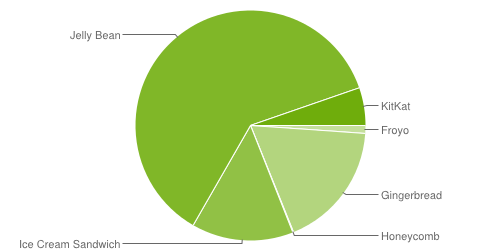
\includegraphics[width=.75\textwidth]{figuras/introducao/chart.png}
  \caption{Distribuição das vendas do Android em 1 de abril de 2014.}
  \label{fig:distribuicaoAndroid}
\end{figure}

Esse material irá cobrir alguns tópicos no desenvolvimento de aplicativos para Android, tais como:
\bi
  \item Configuração do ambiente de desenvolvimento: Como configurar o ambiente para começar a desenvolver aplicativos, os primeiros passos para criar seu primeiro aplicativo de maneira simples;
  \item Elementos da interface: Como projetar seu aplicativo para usar as principais interfaces. Listas, Listas compostas, Grades, Abas, Menus são as interfaces mais usadas nos diversos aplicativos no mercado; e
  \item Elementos de hardware: Como projetar seu aplicativo para usar as APIs de hardware: Bluetooth, GPS, SMS, Chamadas.
\ei

Para esse material, algumas convenções serão seguidas: 
\bi
  \item Os códigos estarão sempre com a sintaxe colorida para facilitar a leitura;
  \item URLs das referências estarão nas notas de rodapé; e
  \item Dicas estarão envoltas por uma caixa para facilitar a visualização.
\ei

\newpage

\section{Configuração do Ambiente}

A instalação e configuração do ambiente de desenvolvimento para Android é simples, o Google fornece um pacote chamado ADT \emph{(Android Development Tools)} que contém o ambiente Eclipse com o \emph{plugin} do Android, algumas ferramentas para instalação dos aplicativos nos \emph{smartphones}, o gerenciador do SDK e as imagens para o emulador do Android.

\singlespace

\textbf{O pacote completo que deve ser instalado é:}
\begin{itemize}
\item \href{http://developer.android.com/sdk/}{Eclipse ADT}\footnote{\href{http://developer.android.com/sdk/}{http://developer.android.com/sdk/}}.
\item \href{http://goo.gl/X68FzJ}{JDK}\footnote{\href{http://goo.gl/X68FzJ}{http://goo.gl/X68FzJ }}. 
\item \href{http://developer.android.com/sdk/}{JRE}\footnote{\href{http://developer.android.com/sdk/}{http://developer.android.com/sdk/}}. 
\end{itemize}

\textbf{Após a instalação será necessário abrir o \emph{SDK Manager} e instalar::}
\begin{itemize}
\item Android SDK Tools.
\item Android SDK Platform-Tools.
\item Android 4.4.2 (API 19).
\end{itemize}

\doublespace

E para cada API que você irá utilizar, instalar o \emph{SDK Platform} e opcionalmente o \emph{Documentation for Android SDK} e o \emph{Samples for SDK}

Para padronizar as operações futuras, as aplicações serão configuradas para a API 19, para download abra o Android SDK Manager e marque o item \emph{Android 4.4.2 (API 19)} e clique para instalar o pacote. Algumas configurações vão necessitar de certas API's, caso queira utilizar seu aparelho para testar as aplicações por exemplo, baixe o \emph{Google USB Driver} do grupo \emph{Extras}.

\chapter{Conhecendo a linguagem}
\section{Linguagem}
A linguagem usada para programar na plataforma Android é Java. Então, antes de engajar no aprendizado Android é recomendável estudar algum material sobre Java e principalmente o paradigma de orientação a objetos.

O Android tem algumas particularidades na organização e configuração que é feita através de arquivos XML específicos do Android. Alguns arquivos XML servem para configurar o aplicativo, layout de cada tela e outros dão suporte a strings para facilitar o suporte a múltiplos idiomas. Felizmente o conjunto Eclipse com ADT já cuida disso automaticamente e possui uma série de facilidades alcançadas por meio de interfaces gráficas para os programadores. Por esse motivo, para qualquer iniciante nessa área é recomendável a utilização do ambiente Eclipse.

A criação de layouts dos aplicativos pode ser feita inteiramente através da interface gráfica disponível no ambiente, no estilo \textit{drag and drop}. 

\section{Entendendo a estrutura de uma aplicação Android}

Uma aplicação Android consiste de uma ou mais \emph{activities}. Uma \emph{activity} é uma tela com \emph{views} que interagem com o usuário. Como o Android segue o padrão MVC \emph{(Model-View-Control)} as \emph{activities} são os \emph{controllers} e as \emph{views}, \emph{views}. As \emph{activities} são classes do Java, o \emph{layout} e outros recursos são definidos em arquivos XML.

Dentre os diversos arquivos XML existentes na configuração de um aplicativo Android o mais importante é o \texttt{{AndroidManifest.xml}}
\footnote{Documentação do \texttt{AndroidManifest}: \href{The AndroidManifest.xml File}{http://developer.android.com/guide/topics/manifest/manifest-intro.html}}
 pois é nele que se exprimem as configurações gerais do aplicativo. Nesse texto não iremos adentrar muito nos detalhes das configurações, mas apenas deixar claro que é nesse arquivo que se colocam as versões do Android que seu aplicativo será compatível com, as permissões para usar os recursos do aparelho como Internet, GPS, Bluetooth, etc. 
 
 A pasta \texttt{src/} contém o pacote com as classes do seu aplicativo isto é, o código fonte do seu aplicativo. Tanto \emph{activites} como classes de suporte devem estar dentro do pacote.

Dentro da pasta \texttt{res/} de recursos, encontram-se outros arquivos, referentes à disposição do layout, valores de strings e imagens que sua aplicação irá utilizar. A pasta \texttt{layout/} junto com as pastas \texttt{drawable/} servem para dispor o layout. Cada \textit{drawable} comporta imagens para um tamanho diferente de tela, enquanto que a pasta de \textit{layout} contém a disposição geral do layout. São nesses arquivos que se colocam os itens \emph{(views)} que irão nas telas, como botões, caixas de texto, caixas de seleção, etc.

Na pasta \texttt{values/} o mais importante é o arquivo \texttt{strings.xml} que contém os valores das strings do aplicativo. Sempre que você quiser referenciar alguma string, a mesma deverá estar expressa nesse arquivo. Fica fácil dessa forma fazer o aplicativo suportar múltiplos idiomas, pois basta traduzir esse único arquivo para alterar todos os textos do aplicativo.

A pasta \texttt{menu/} contém os \emph{layouts} do menus do aplicativo, esses são aqueles que podem ser acessados através da \emph{Action Bar}\footnote{\emph{ActionBar}: \href{http://developer.android.com/design/patterns/actionbar.html}{http://developer.android.com/design/patterns/actionbar.html}} ou através dos botões físicos do aparelho.

\section{Alguns arquivos importantes:}

\textbf{/res/layout/activity\_main.xml:}

O arquivo \emph{activity\_main.xml} localizado na pasta \emph{layout} define a interface gráfica da tela. Por padrão, ao criar o projeto esse arquivo contém uma tag \emph{<TextView>} para exibir um simples texto na tela. Essa tag define o atributo \emph{android:text="\@string/hello"}, que utiliza uma mensagem identificada pela chave hello localizada no arquivo \emph{strings.xml}.

\textbf{/res/values/strings.xml:}

O arquivo \emph{strings.xml} localizado na pasta \emph{values} contém as mensagens da aplicação para organizar os textos em um único arquivo centralizado, o que é uma boa prática de programação. Desta forma podemos facilmente traduzir este arquivo para diversos idiomas e tornar nossa aplicação bastante internacionalizáveis.
Por padrão, esse arquivo contém o nome da aplicação que digitamos ao criar o projeto e a mensagem que aparece na tela principal definida pelo arquivo \emph{main.xml}.
O nome da aplicação é definido pela chave \emph{app\_name}, e o texto que aparece na tela é definido pela chave \emph{hello}.  O padrão para acessar essas mensagens é @string/nomeDaChave.
Se for necessário mais de um idioma no aplicativo, basta criar uma pasta /res/values/values-(código do idioma) e traduzir o arquivo \emph{strings.xml} desta pasta.

\textbf{R.java:}

A classe \emph{R} tem constantes para facilitar acesso aos recursos do projeto, como por exemplo, um arquivo XML que define uma tela ou uma imagem localizada na pasta \emph{drawable}.
Sempre que um recurso é adicionado no projeto, como por exemplo, uma nova imagem, essa classe é gerada automaticamente pelo Eclipse para conter uma constante para o novo recurso criado. \textbf{Nunca altera a classe R manualmente!} 

\textbf{MainActivity.java:}

Esta é a classe principal do projeto e representa a tela inicial da aplicação. Observe que essa classe é filha de \emph{android.app.Activity}.
A classe \emph{android.app.Activity} representa uma tela da aplicação e é responsável por controlar o estado e os eventos da tela. Assim, para cada tela da aplicação você criará uma classe-filha de \emph{Activity}. O método \emph{onCreate(bundle)} precisa ser implementado obrigatoriamente e é chamado de forma automática pelo Android quando a tela é criada. No entanto, a classe \emph{android.app.Activity} não sabe desenhar nada na tela e para isso precisa da ajuda da classe \emph{android.view.View} que, por sua vez, se encarrega de desenhar os componentes visuais, como campos de texto, botões e imagens. Para isso, existem diversas subclasses especializadas de \emph{android.view.View}.

\textbf{AndroidManifest.xml:}

O arquivo \emph{AndroidManifest.xml} é o arquivo principal do projeto e centraliza as configurações da aplicação. Note que existe, no arquivo xml a tag \emph{uses-sdk} a qual é utilizada para informar o level mínimo da API exigido pela aplicação. Por exemplo, uma aplicação pode ser compatível com a API level 8 mas otimizado para a 19, isto é, o Android 4.4: \emph{<uses-sdk android:minSdkVersion="8"   android:targetSkdVersion="19"  />}



\textbf{Resumindo:}
\begin{itemize}
\item \texttt{AndroidManifest.xml}: Configurações gerais do aplicativo;
\item \texttt{src/}: Classes do aplicativo; e
\item \texttt{res/}: Recursos do aplicativo tais que:
	\begin{itemize}
		\item \texttt{strings/}: Todos os textos da sua aplicação, suporte a múltiplos idiomas;	
		\item \texttt{layout/}: Todos os \emph{layouts} de suas telas \emph{(activites)};
		\item \texttt{drawable/}: Todas as imagens, separados por tamanho de tela; e
		\item \texttt{menu/}: \emph{layout} dos menus do aplicativo.
	\end{itemize}
\end{itemize}

%First App
\section{Criando seu primeiro aplicativo}
Para exemplificar a criação de um aplicativo, seguiremos o exemplo dado pelo próprio manual do Google sobre o Android 
(Ver original\footnote{Original em: \href{http://developer.android.com/training/basics/firstapp/creating-project.html}{http://developer.android.com/training/basics/firstapp/creating-project.html}}). 
Trata-se de aplicativo simples do tipo \emph{''Hello World''}.

Iniciaremos criando um novo projeto no Eclipse acessando o menu: \emph{File -> New -> Android Application Project}.

Na janela que apareceu você deve colocar o nome do aplicativo, do projeto e do pacote. O nome do pacote deve seguir a convenção do Java\footnote{Convenção sobre nome dos pacotes: \href{http://docs.oracle.com/javase/tutorial/java/package/namingpkgs.html}{http://docs.oracle.com/javase/tutorial/java/package/namingpkgs.html}}.
\begin{itemize}
	\item \textit{Minimum Required SDK:} É a versão mínima do sistema operacional Android que sua aplicação irá suportar, o mais comum é a versão 8 do SDK que se refere ao Android 2.2. Alguns tipos de layouts mais complexos não são suportados em versões mais antigas;
	\item \textit{Target SDK:} É a versão principal do Android para qual seu aplicativo está sendo desenvolvido;
	\item \textit{Compile With:} Versão do Android com qual seu aplicativo será compilado, no nosso caso deixe como API 19;
	\item \textit{Theme:} Cores do layout.
\end{itemize}

Observe na \autoref{fig:firstapp1} a janela de criação de uma nova aplicação Android. Em \emph{Application Name} você deve colocar o nome do aplicativo, em \emph{Project Name}, o nome do projeto e em \emph{Package Name} o nome do pacote. Para esse exemplo utilizaremos como \emph{Minimum Required SDK} a versão API 8, já que nesse exemplo não usaremos nenhum layout que não é suportado em versões mais antigas. Em \emph{Target SDK} e \emph{Compile With} optaremos pela versão mais nova, a API 17. Por final o \emph{Theme} eu optei pelo \emph{Holo Light with Dark Action Bar} que é um tema com fundo branco e barra superior preta, um dos padrões do Android.

\begin{framed}
\textbf{Dica:} Para obter o máximo de compatibilidade sempre procure utilizar \emph{layouts} compatíveis com versões antigas, observe na \autoref{fig:distribuicaoAndroid} que versões antigas ainda tem uma fatia considerável do mercado.
\end{framed}

\begin{figure}[H]
  \centering
  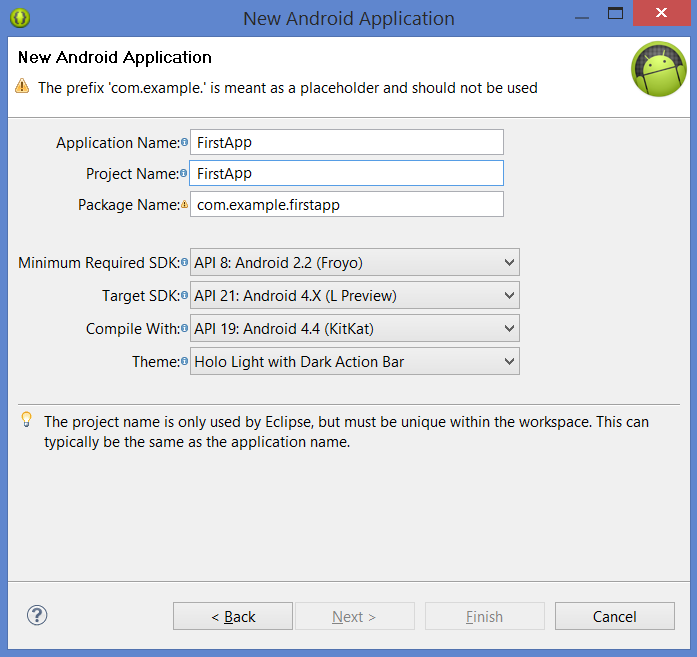
\includegraphics[width=.75\textwidth]{figuras/firstapp/firstapp1.png}
  \caption{Primeira janela de criação de novo aplicativo}
  \label{fig:firstapp1}
\end{figure}


A \autoref{fig:firstapp2} mostra a segunda janela da configuração inicial do seu aplicativo. 

\begin{figure}[H]
  \centering
  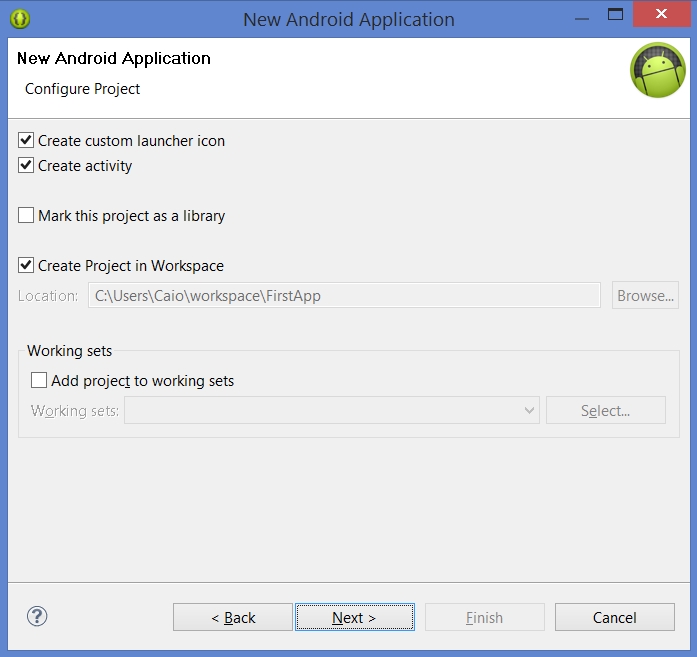
\includegraphics[width=.75\textwidth]{figuras/firstapp/firstapp2.png}
  \caption{Segunda janela de criação de novo aplicativo}
  \label{fig:firstapp2}
\end{figure}


Você pode escolher um ícone personalizado se marcar a caixa \emph{Create custom launcher icon} o que te levará para a janela da \autoref{fig:firstapp3}. 

\begin{figure}[H]
  \centering
  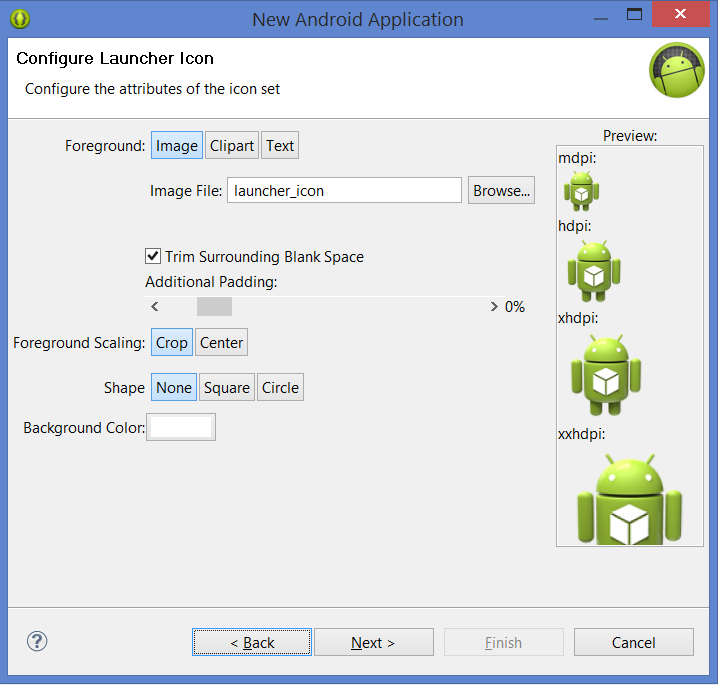
\includegraphics[width=.75\textwidth]{figuras/firstapp/firstapp3.png}
  \caption{Terceira janela de criação de novo aplicativo}
  \label{fig:firstapp3}
\end{figure}
  
Se marcar \emph{Create Activity}  o assistente de criação te levará para a janela da \autoref{fig:firstapp4} onde poderá escolher qual \emph{activity} vai ser criada para seu aplicativo. Em todos os exemplos escolheremos a opção \emph{Blank Activity}. Como nosso projeto não é uma biblioteca não marcaremos \emph{Mark this project as a library}. Se marcar \emph{Create Project in Workspace} o assistente irá salvar o projeto na pasta que foi configurada para o \emph{Workspace}, caso contrário ele irá pedir para escolher outro caminho. Como não trabalharemos com \emph{Working Sets} do Eclipse, a opção \emph{Add project to working sets} permanece desmarcada. 
  
\begin{figure}[H]
  \centering
  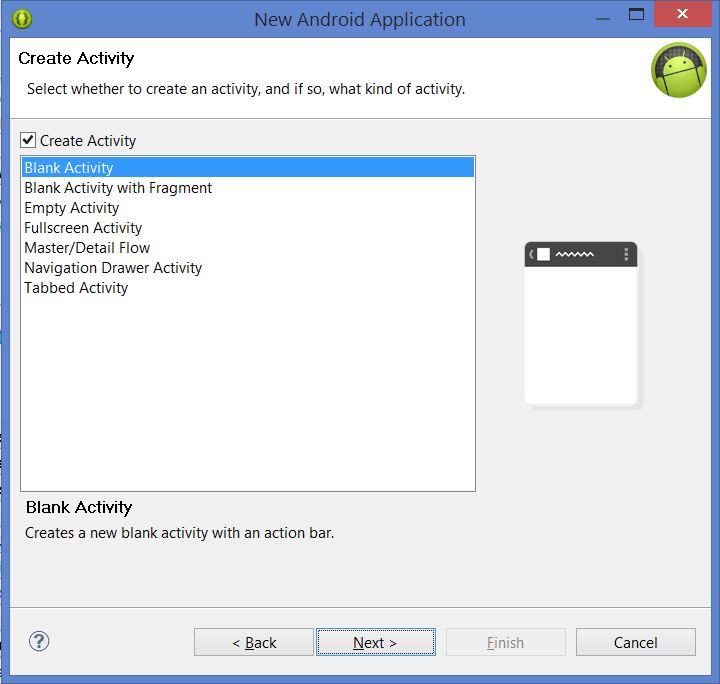
\includegraphics[width=.75\textwidth]{figuras/firstapp/firstapp4.png}
  \caption{Quarta janela de criação de novo aplicativo}
  \label{fig:firstapp4}
\end{figure}
 
Finalmente a \autoref{fig:firstapp5} mostra a janela para nomear a \emph{activity} inicial, nesse exemplo mantive \emph{MainActivity}. O nome do \emph{layout} dessa \emph{activity} mantive como \emph{activity\_main} que é o padrão. Na caixa \emph{Navigation Type} existem algumas opções de \emph{layout} pré-definidas pelo Android. São elas:
\begin{itemize}
\item
	\emph{None:} O \emph{layout} vem apenas com uma \emph{Action Bar}\footnote{Documentação da \emph{ActionBar}: \href{http://developer.android.com/guide/topics/ui/actionbar.html}{http://developer.android.com/guide/topics/ui/actionbar.html}}
\item
	\emph{Fixed Tabs + Swipe:} O \emph{layout} vem com algumas abas e com gesto de arrastar entre as abas \emph{(activities)} pré-programados.
	\footnote{\emph{Tabs:} \href{http://developer.android.com/design/building-blocks/tabs.html}{http://developer.android.com/design/building-blocks/tabs.html}}
\item
	\emph{Scrollable Tabs + Swipe:} O \emph{layout} vem com algumas abas e com gesto de arrastar entre as abas pré-programados, porém nesse o estilo das abas é diferente, em vez de abas fixas, são abas que movem para dar espaço a outras. 
\item
	\emph{Dropdown}: O \emph{layout} vem com a troca de \emph{activites} através de um menu na \emph{Action Bar}.  
\end{itemize}


\begin{figure}[H]
  \centering
  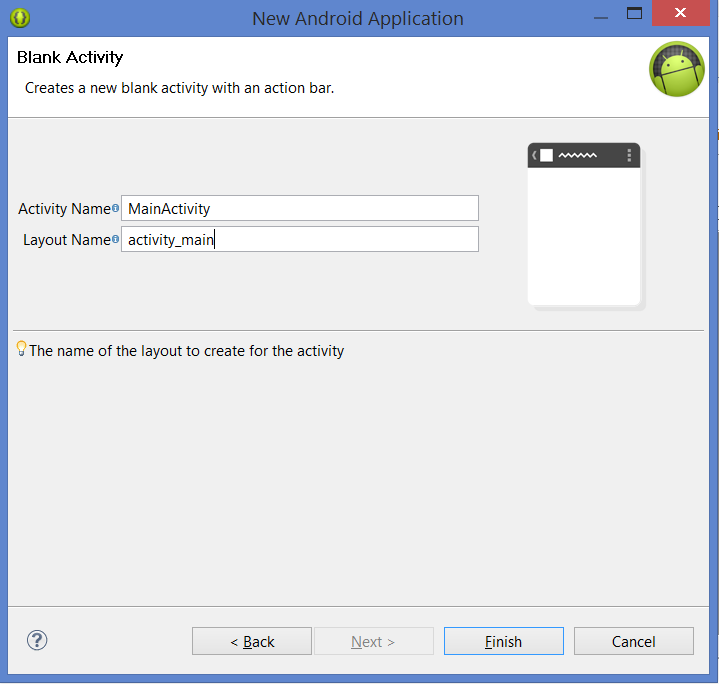
\includegraphics[width=.75\textwidth]{figuras/firstapp/firstapp5.png}
  \caption{Quinta janela de criação de novo aplicativo}
  \label{fig:firstapp5}
\end{figure}


Você pode configurar a versão do SDK manualmente modificando os valores no \emph{manifest}. Como mostrado no exemplo abaixo:


\begin{listing}[H]
\inputminted[linenos=true,fontsize=\small,frame=lines, framesep=2mm, tabsize=2,numbersep=5pt]{xml}{src/firstapp/sdk-manifest.xml}
\label{AndroidManifest.sdk}
\caption{Exemplo de configuração de versão do SDK no arquivo \texttt{AndroidManifest.xml} }
\end{listing}

A tag \texttt{uses-sdk} serve apenas para o compilador saber quais versões do Android você pretende que seu aplicativo suporte. Dessa forma quando seu aplicativo for lançado na loja \emph{Google Play} o aplicativo só será visível para aqueles usuários que possuem a versão mínima do Android indicada no atributo.

Primeiro vamos criar um \emph{layout} para o aplicativo usando o construtor de interfaces presente no ambiente, primeiro abra o arquivo \texttt{res/layout/activity\_main.xml} , segundo o \emph{manifest}, é essa \emph{activity} que será aberta quando o aplicativo for iniciado, isso é configurado através do \emph{intent-filter}\footnote{Mais informações na \hyperref[sec:especac]{Seção \ref*{sec:especac}}}. 

Selecione o ''Hello world'' e o remova da sua \emph{activity}.

\begin{figure}[H]
  \centering
  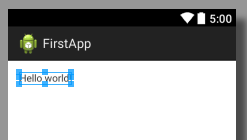
\includegraphics[width=.4\textwidth]{figuras/firstapp/firstapp6.png}
  \caption{Selecionando o Hello World}
  \label{fig:firstapp6}
\end{figure}

Antes de continuar, altere a API selecionada por padrão para a 19 conforme a figura \autoref{fig:changeAPI} (ou outra menor, é possível instalar as versões através do \emph{Android SDK Manager}).

\begin{figure}[H]
  \centering
  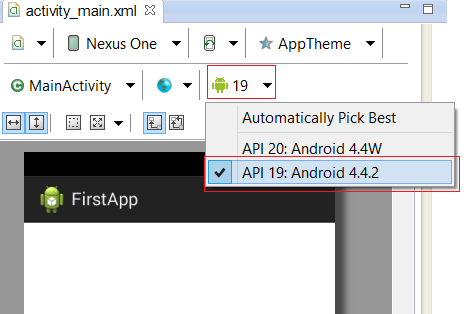
\includegraphics[width=.5\textwidth]{figuras/firstapp/changeAPI.png}
  \caption{Alterando API padrão}
  \label{fig:changeAPI}
\end{figure}


A tela deverá ficar parecida com a \autoref{fig:firstapp6}. Agora arraste um \textit{Text Field -> Plain Text} e um \textit{Form Widgets -> Button} para sua \emph{activity}.


\begin{figure}[H]
  \centering
  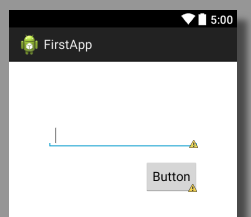
\includegraphics[width=.4\textwidth]{figuras/firstapp/firstapp7.png}
  \caption{\emph{activity} com os elementos colocados na tela}
  \label{fig:firstapp7}
\end{figure}

Ao clicar duas vezes no elemento no modo visual, você será levado ao marcador desse elemento no XML correspondente da \emph{activity}. Clique duas vezes na caixa de texto, o seguinte código será exibido:

\begin{listing}
\inputminted[linenos=true,fontsize=\small,frame=lines, framesep=2mm, tabsize=2,numbersep=5pt]{xml}{src/firstapp/1.xml}
\caption{Código da caixa de texto no arquivo \texttt{activity\_main.xml}}
\end{listing}

Primeiro, na linha 2 modifique o \emph{id} do \emph{Text Field} para um nome mais intuitivo, nesse exemplo chamaremos apenas de \emph{nameField}. O Android definiu que todo novo atributo \emph{id} deve ser precedido de \texttt{@+id/}. O símbolo @ diz para o compilador que estamos acessando os recursos do Android, esses recursos são compilados na classe \texttt{R} automaticamente. O símbolo + diz para o compilador que estamos criando um novo recurso. Por fim, \emph{id} diz que estamos especificando um novo identificador para esse recurso e só então damos o nome a esse identificador.

\begin{framed}
\textbf{Dica:} Existem vários tipos de recursos, porém é importante salientar os diferentes tipos de \emph{id}. Quando referimos aos recursos podemos usar \texttt{@android:id/} para acessar recursos que já estão definidos no sistema Android. Usamos \texttt{@id/} para acessar recursos que já foram definidos no seu projeto. Para criar um novo recurso, usamos \texttt{@+id/}.
\end{framed}

Os outros atributos são para definir o tamanho, alinhamento e margem da caixa de texto. O valor \texttt{wrap\_content} dos atributos \texttt{layout\_width} e \texttt{layout\_height} (largura e altura, linhas 3 e 4) força a \emph{view} a mudar de tamanho automaticamente para abrigar seu conteúdo. Os atributos \texttt{layout\_alignParentLeft} e \texttt{layout\_alignParentTop} servem (linhas 5 e 6) para alinhar essa \emph{view} com a \emph{view} pai dela, dessa forma ficará alinhado com a borda esquerda e com a borda superior do pai. Os atributos \texttt{layout\_marginLeft} e \texttt{layout\_marginTop} (linhas 7 e 8) deslocam o elemento colocando uma margem entre a borda e a \emph{view}, esses valores estarão diferentes pois são computados automaticamente quando a \emph{view} é colocada através do construtor de interfaces. Note que isso só acontecerá caso esteja usando \texttt{RelativeLayout}\footnote{Mais informações na \hyperref[subsec:relativelayout]{Seção \ref*{subsec:relativelayout}}} que é o nosso caso. Por último o atributo \texttt{ems} (linha 9) configura o tamanho da fonte através da unidade de medida Em.

Depois adicione uma \textit{hint} para essa caixa de texto, uma \textit{hint} é algo que vai estar escrito na caixa de texto quando ela estiver vazia, indicando que tipo de texto você pretende que seja escrito nessa caixa de texto, Neste exemplo (linha 10) a \textit{hint} é uma referência a \emph{string} chamada \emph{name} que iremos definir depois.

Depois modifique o código do botão que está no mesmo arquivo, troque o \emph{id} do botão (linha 2), também edite o atributo \texttt{text} (linha 8) para fazer uma referência a uma \emph{string} definida no arquivo de \emph{strings} que iremos chamar de \emph{send\_button}. Por último adicione um atributo \texttt{onClick} (linha 9) que define o método que será chamado quando esse botão for pressionado.

\begin{listing}[H]
\inputminted[linenos=true,fontsize=\small,frame=lines, framesep=2mm, tabsize=2,numbersep=5pt]{xml}{src/firstapp/2.xml}
\caption{Código do botão}
\end{listing}

Agora iremos definir as \emph{strings} usadas anteriormente no arquivo \texttt{res/values/strings.xml}. Abra ele e o modifique para que fique como mostrado no 
\hyperref[code:arquivo-strings]{Algoritmo \ref*{code:arquivo-strings}}

\begin{listing}
\inputminted[linenos=true,fontsize=\small,frame=lines, framesep=2mm, tabsize=2,numbersep=5pt]{xml}{src/firstapp/3.xml}
\caption{Arquivo de strings com as duas strings adicionadas}
\label{code:arquivo-strings}
\end{listing}

Após terminar abra a classe \texttt{MainActivity.java} localizada na pasta (navegue utilizando o explorador de arquivos)
\texttt{src/com.example.firstapp/} do seu projeto e adicione um novo método que chamei de \emph{sendMessage}, ele será responsável por obter o conteúdo da caixa de texto e enviar para uma nova \emph{activity} que irá mostrar esse conteúdo.

\begin{listing}
\inputminted[linenos=true,fontsize=\small,frame=lines, framesep=2mm, tabsize=2,numbersep=5pt]{java}{src/firstapp/4.java}
\caption{Adicionando método à classe MainActivity}
\end{listing}

\begin{framed}
\textbf{Dica:} Isso vai requer você importe a classe View, você pode apertar \texttt{Ctrl+Shit+O} no Eclipse para importar classes que estejam faltando
\end{framed}

\begin{listing}
\inputminted[linenos=true,fontsize=\small,frame=lines, framesep=2mm, tabsize=2,numbersep=5pt]{java}{src/firstapp/4-2.java}
\caption{Exemplo de import de uma classe Android}
\end{listing}

Primeiro, crie um novo \texttt{Intent}\footnote{Documentação Intent: \href{http://developer.android.com/reference/android/content/Intent.html}{http://developer.android.com/reference/android/content/Intent.html}}, um \texttt{Intent} é um objeto que provê uma facilidade para realizar uma ligação entre códigos de diferentes aplicações. O uso mais significtivo é a inicialização de novas \emph{activities}.

\begin{listing}[H]
\inputminted[linenos=true,fontsize=\small,frame=lines, framesep=2mm, tabsize=2,numbersep=5pt]{java}{src/firstapp/5.java}
\caption{Adicionando uma \texttt{Intent}}
\label{code:obtendo-intent}
\end{listing}

É necessário realizar outro \emph{import} como indicado pelo \hyperref[code:importTI]{Algoritmo \ref*{code:importTI}}.
Agora iremos obter o texto que está escrito na caixa para fazer algo com ele, no caso iremos enviar para outra \emph{activity} que irá mostrar esse texto. Como é feito no \hyperref[code:obtendo-intent2]{Algoritmo \ref*{code:obtendo-intent2}}.

\begin{listing}[H]
\inputminted[linenos=true,fontsize=\small,frame=lines, framesep=2mm, tabsize=2,numbersep=5pt]{java}{src/firstapp/6.java}
\caption{Obtendo o conteúdo da caixa de texto e enviando para outra \emph{activity}}
\label{code:obtendo-intent2}
\end{listing}

O código na linha 3 está obtendo a referência da caixa de texto usando o método \\ \texttt{findViewById()} passando o \textit{id} da caixa de texto como parâmetro, esse \emph{id} é obtido acessando uma variável estática da classe \texttt{R}  (observe que esse e o mesmo \emph{id} que voce colocou no arquivo xml do layout da \emph{activity}).
Em seguida usando o método \texttt{getText()} da caixa de texto, obtém-se a \emph{string} que foi escrita pelo usuário.

Por fim, essa \emph{string} é colocada no \texttt{Intent} com o método \texttt{putExtra()}, uma \texttt{Intent} pode carregar consigo uma coleção de vários tipos de dados como pares chave-valor chamados \textit{extras}, esse método toma a chave como primeiro parâmetro e o valor no segundo parâmetro.
Para que a próxima \emph{activity} consiga coletar esse valor, você deve definir uma chave para seu \textit{extra} usando uma constante pública. Para isso adicione a definição de \texttt{EXTRA\_MESSAGE} no topo da sua classe \texttt{MainActivity}.

\begin{listing}[H]
\inputminted[linenos=true,fontsize=\small,frame=lines, framesep=2mm, tabsize=2,numbersep=5pt]{java}{src/firstapp/7.java}
\caption{Constante como chave para um extra}
\end{listing}

Pode ser necessário adicionar o \emph{import} manualmente, basta adicionar conforme o \hyperref[code:importTI]{Algoritmo \ref*{code:importTI}} antes da declaração da \emph{public class MainActivity ...}.

\begin{listing}[H]
\inputminted[linenos=true,fontsize=\small,frame=lines, framesep=2mm, tabsize=2,numbersep=5pt]{java}{src/firstapp/10.java}
\caption{\emph{import} para o \emph{Intent}}
\label{code:importTI}
\end{listing}

Agora você deve criar uma nova \emph{activity}, para isso vá em \textit{File -> New -> Other -> Android Activity} e selecione \textit{Blank Activity}. Preencha a próxima janela como na \autoref{fig:firstapp8}, depois clique \textit{Finish}. 

\begin{figure}[H]
  \centering
  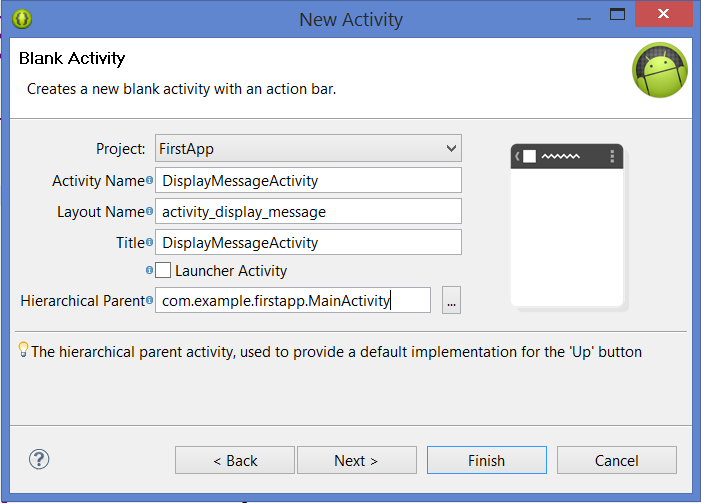
\includegraphics[width=.75\textwidth]{figuras/firstapp/firstapp8.png}
  \caption{Criando uma nova \emph{activity}}
  \label{fig:firstapp8}
\end{figure}

Observe na \autoref{fig:firstapp8}. Em \emph{Project} você vai especificar o projeto em que a nova \emph{activity} será adicionado. Em \emph{Activity Name} especifique o nome da sua nova \emph{activity}. Em \emph{Layout Name} defina o nome do arquivo XML que contém o \emph{layout} da nova \emph{activity}. A opção \emph{Title} define o título da \emph{activity}, isso pode ser modificado posteriormente no arquivo de \emph{strings} pois o título será definido ali após a criação da \emph{activity}. A opção \emph{Launcher Activity} ficará desmarcada pois essa \emph{activity} não será usada para inicializar o aplicativo. Em \emph{Hierarchical Parent} você vai definir o pai da nova \emph{activity}, isso é usado para o Android implementar corretamente para qual \emph{activity} o botão de voltar irá voltar. Por último \emph{Navigation Type} deixe como \emph{None} pois só queremos o \emph{design} padrão. Clique em \emph{Finish} para criar a nova \emph{activity}.
 
 % nota/dica necessaria?
\begin{framed}
\textbf{Dica:} O Eclipse adiciona automaticamente \emph{activities} criadas por esse método no \emph{Manifest}. Observe no \emph{Manifest} como é feito caso você precise adicionar manualmente.
\end{framed}

Abra a nova classe que foi criada junto com a \emph{activity}. A classe já vem com alguns métodos implementados, alguns não serão necessários para esse aplicativo e serão explicados em outras seções, mas mantenha-os na classe. Todas as classes que são subclasses de \emph{Activity} precisam implementar o método \texttt{onCreate()}\footnote{\href{http://developer.android.com/reference/android/app/Activity.html\#onCreate(android.os.Bundle)}{http://developer.android.com/reference/android/app/Activity.html\#onCreate(android.os.Bundle)}} que define o procedimento a ser executado quando a \emph{activity} é criada.

Agora, precisamos extrair os dados enviados a essa \emph{activity} através do \emph{intent}, você pode obter a referência do \emph{intent} que começou a \emph{activity} chamando o método \texttt{getIntent()}\footnote{\href{http://developer.android.com/reference/android/app/Activity.html\#getIntent()}{http://developer.android.com/reference/android/app/Activity.html\#getIntent()}}.

\begin{listing}[H]
\inputminted[linenos=true,fontsize=\small,frame=lines, framesep=2mm, tabsize=2,numbersep=5pt]{java}{src/firstapp/8.java}
\caption{Obtendo a \emph{string} passada como extra do \texttt{Intent}}
\label{code:obtendo-string-intent}
\end{listing}


Repare que na linha 15 alteramos a chamada do o método \texttt{setContentView} que era, originalmente serve para exibir o conteúdo da segunda tela (se você adicionar componentes a ela, será esse visual que será mostrado). Mas para o exercício a exibição ficou restrita a um\texttt{TextView}, caso você queira exibir a segunda tela propriamente dita deixe a chamada como o modelo original (para seguir com o exemplo deixe como definido no algoritmo \hyperref[code:metodoSegundaActivity]{Algoritmo \ref*{code:metodoSegundaActivity}}).

Após obter a referência do \texttt{intent} que iniciou a \texttt{activity}, queremos coletar os extras que foram passado junto com ele. Criamos uma \texttt{string} que irá armazenar a mensagem que veio junto do \texttt{intent} e chamamos o método \texttt{getStringExtra()} passando como parâmetro a chave desse extra, que definimos na classe \texttt{MainActivity}. 
Agora para mostrar a mensagem na tela, você precisa criar um \texttt{TextView}\footnote{\href{http://developer.android.com/reference/android/widget/TextView.html}{http://developer.android.com/reference/android/widget/TextView.html}}, essa \texttt{view} serve para mostrar texto. 


\begin{listing}[H]
\inputminted[linenos=true,fontsize=\small,frame=lines, framesep=2mm, tabsize=2,numbersep=5pt]{java}{src/firstapp/9.java}
\caption{Método \texttt{onCreate()} recebendo um \emph{Intent} e mostrando a mensagem}
\label{code:metodoSegundaActivity}
\end{listing}

As linhas 1, 2 e 3 foram colocadas automaticamente na criação da \emph{activity}, a linha 3 faz uma chamada ao método da superclasse.

O \hyperref[code:metodoSegundaActivity]{Algoritmo \ref*{code:metodoSegundaActivity}} foi colocado nas linhas 6 e 7 para obter a referência ao \emph{Intent}. Nas linhas 10-12 criamos um novo \texttt{TextView}, configuramos o tamanho da fonte e atribuímos o texto que será mostrado na tela a \emph{view}, respectivamente. 

\newpage

Agora que o aplicativo está pronto, é necessário testar, caso tenha um smartphone Android você pode conectá-lo no seu computador e rodar diretamente, senão você deverá rodar em um emulador. Lembrando que para ambos os casos é necessária a instalação do SDK primeiro, acesse \emph{Android SDK Manager} e faça o download do SDK desejado.

Para rodar diretamente no smartphone:
\be
\item Conecte seu smartphone no computador através do cabo USB. Se estiver desenvolvendo no Windows será preciso instalar os drivers USB do seu dispositivo (\emph{driver ADB}). Se precisar de ajuda para instalar os drivers acesse: \href{http://developer.android.com/tools/extras/oem-usb.html}{OEM USB}\footnote{\href{http://developer.android.com/tools/extras/oem-usb.html}{http://developer.android.com/tools/extras/oem-usb.html}}
\item Ative o modo \emph{USB Debugging} no dispositivo
	\bi
	\item Para Android 3.2 ou mais antigos, a opção deve estar em \textit{Configurações -> Aplicativos	 -> Desenvolvimento}
	\item Para Android 4.0 e 4.1, a opção está em \textit{Configurações -> Opções do desenvolvedor}
	\item Para Android 4.2 e mais novos, a opção está escondida por padrão, para mostrar a opção você deve entrar em \textit{Sobre o telefone} e clicar em \textit{Número da versão} 7 vezes, ao retornar para tela anterior deverá aparecer \textit{Opções do desenvolvedor}
	\ei
\item Com o driver instalado e o device devidamente conectado, a única alteração necessária é selecionar o aparelho como \emph{target} para as aplicações desenvolvidas no eclipse.
\ee

A figura \autoref{fig:AddEmulador2} mostra como abrir as opções de execução do aplicativo, na tela \autoref{fig:AddEmulador3} é indicado a aba referente a opção de \emph{target}, depois deve ser selecionado a opção \emph{Always prompt to pick device} como ilustrado na figura \autoref{fig:AddEmulador12} e em seguida \emph{Run}.
Essa opção vai exibir uma tela cada vez que o aplicativo for executado perguntando em qual \emph{device} queremos executar, se tudo estiver de acordo o aparelho será exibido como opção, assim como a figura \autoref{fig:AddEmulador13}.

\begin{figure}[H]
  \centering
  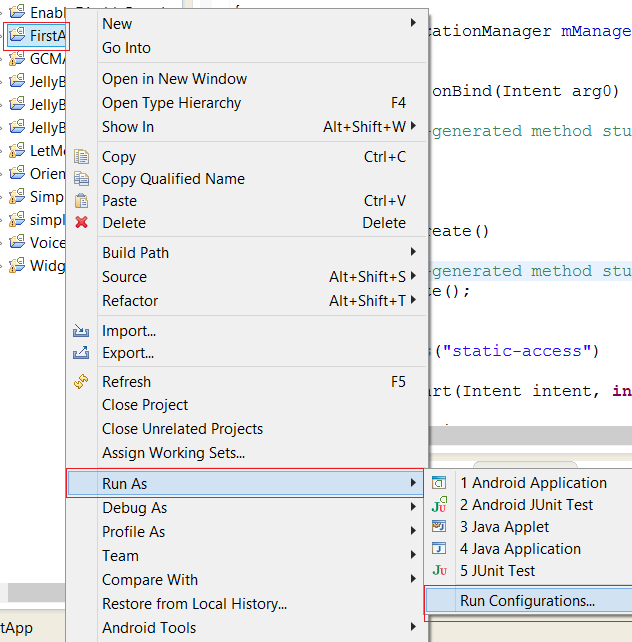
\includegraphics[width=.7\textwidth]{figuras/emulador/AddEmulador2.png}
  \caption{Configurando opções de execução do aplicativo}
  \label{fig:AddEmulador2}
\end{figure}

\begin{figure}[H]
  \centering
  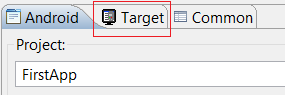
\includegraphics[width=.4\textwidth]{figuras/emulador/AddEmulador3.png}
  \caption{Selecionando projeto para alterar o \emph{Target}}
  \label{fig:AddEmulador3}
\end{figure}

\begin{figure}[H]
  \centering
  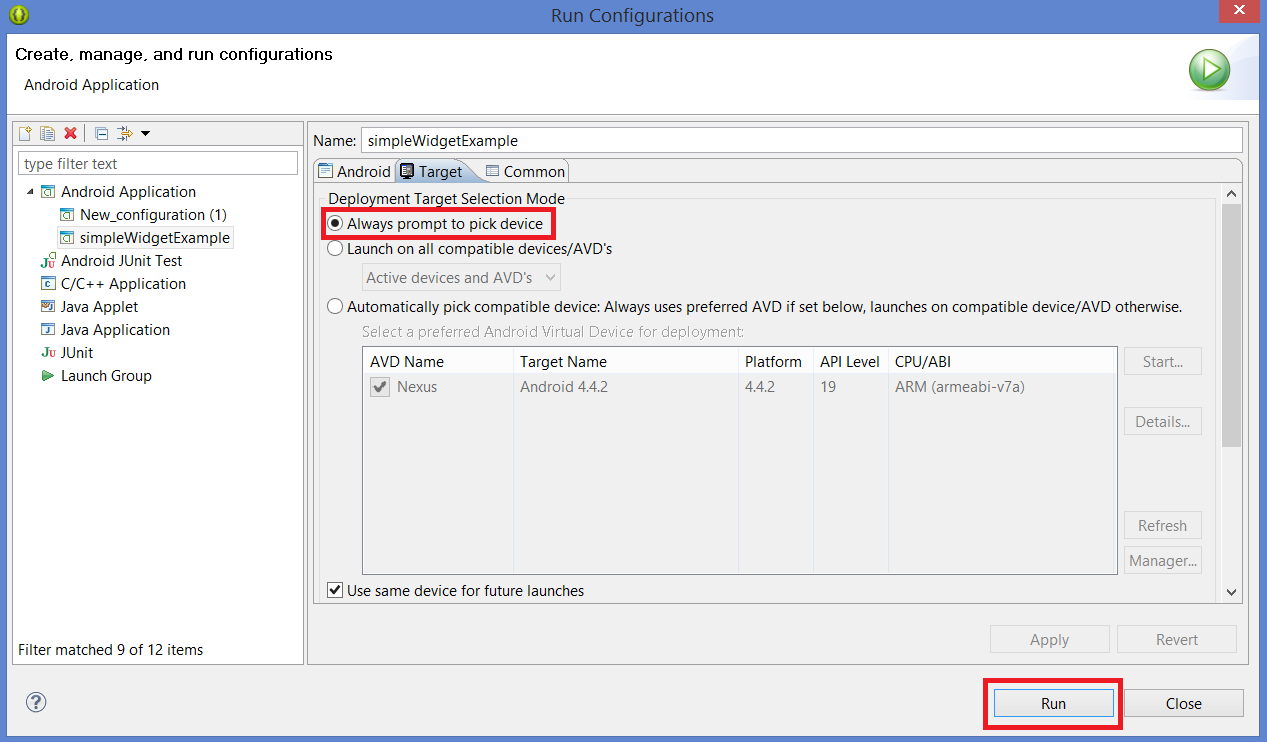
\includegraphics[width=.7\textwidth]{figuras/emulador/AddEmulador12.png}
  \caption{Definindo opção de execução para exibir uma tela de \emph{devices} disponíveis}
  \label{fig:AddEmulador12}
\end{figure}

\begin{figure}[H]
  \centering
  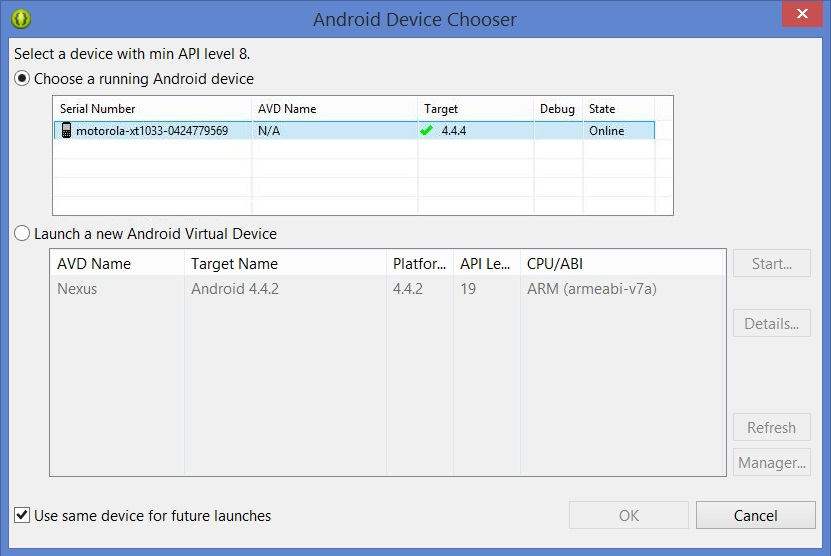
\includegraphics[width=.7\textwidth]{figuras/emulador/AddEmulador13.png}
  \caption{Selecionando o \emph{device} para executar o aplicativo}
  \label{fig:AddEmulador13}
\end{figure}

\begin{framed}
\textbf{Dica:} Caso ocorra o erro \emph{Launch error: adb rejected command: device not found}. Verifique se o aparelho está conectado e se os drivers estão instalados corretamente. Na área de notificações do aparelho deve ter uma notificação escrita: \emph{Android debugging enabled}. 
\end{framed}

\newpage 

\emph{Para rodar no emulador}:

\be
\item Abra o \textit{SDK Manager} através do Eclipse em: \textit{Window -> Android SDK Manager}
\item Verifique se, para Android 4.4.2 (API 19) ou outro desejado os seguintes pacotes estejam instalados
	\bi
	\item \textit{SDK Platform} e;
	\item \textit{ARM EABI v7a System Image} ou;
	\item \textit{Intel x86 Atom System Image}
	\ei
\item Verifique também se na aba \textit{Tools}, os pacotes \textit{Android SDK Tools} e \textit{Android SDK Platform-tools} estão instalados
\item Agora é necessário criar um AVD (Android Virtual Device\footnote{\href{http://developer.android.com/tools/devices/index.html}{http://developer.android.com/tools/devices/index.html}}). No Eclipse acesse o menu \textit{Window -> Android Virtual Device Manager} 
\item No AVD Manager clique em \emph{New}
\item Complete as informações do AVD, especificando um aparelho, nome, plataforma, espaço de armazenamento, quantidade de memória RAM. Em \emph{Device} haverá opções pré-configuradas de aparelhos do google, os \emph{Nexus}, e opções genéricas de acordo com tamanho de tela. Em \emph{Target} você deverá escolher a versão do sistema Android que deseja. Em alguns casos você poderá decidir pela CPU caso deseje ARM ou Intel Atom x86. A quantidade de RAM no Windows fica limitada a 768MB, mais que isso pode acarretar em erros no sistema.

\item Clique \emph{Create AVD}
\item Ainda na janela \emph{Android Virtual Device Manager} selecione o novo AVD e clique \emph{Start}
\item Quando o emulador terminar de carregar, destrave a tela do emulador, usando o mouse.
\ee

%%

\begin{figure}[H]
  \centering
  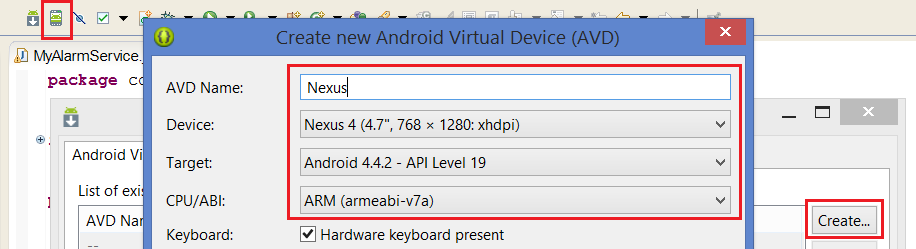
\includegraphics[width=.7\textwidth]{figuras/emulador/AddEmulador1.png}
  \caption{Criando um novo \emph{Virtual Device}}
  \label{fig:AddEmulador1}
\end{figure}


\begin{figure}[H]
  \centering
  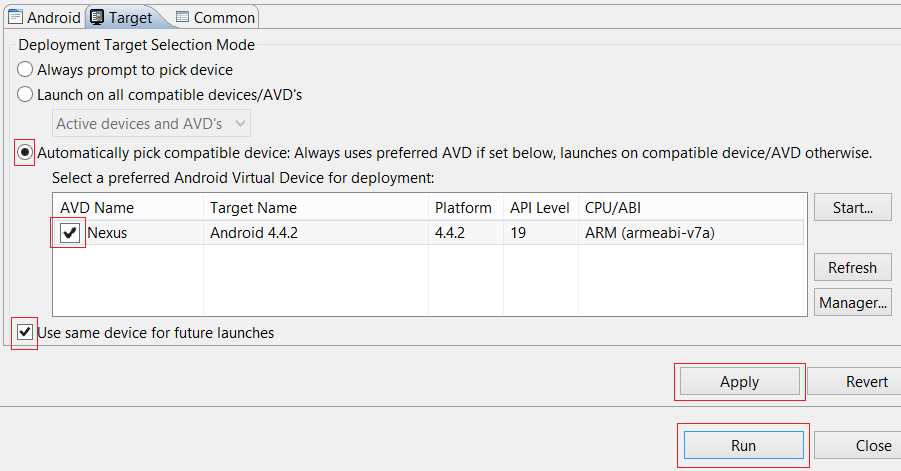
\includegraphics[width=.7\textwidth]{figuras/emulador/AddEmulador4.png}
  \caption{Alterando o \emph{Target} do aplicativo}
  \label{fig:AddEmulador4}
\end{figure}


Agora para rodar o aplicativo basta clicar em \emph{Run} na barra de tarefas do Eclipse e selecionar \textit{Android Application} na janela \emph{Run as}. O Eclipse irá instalar o APK e abrir o aplicativo automaticamente, no dispositivo ou no emulador. As figuras \autoref{fig:firstapp9}, \autoref{fig:firstapp10} e \autoref{fig:firstapp11} mostram a execução do aplicativo.

\begin{figure}[H]
  \centering
  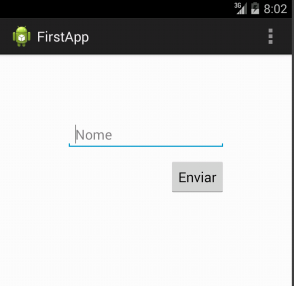
\includegraphics[width=.4\textwidth]{figuras/firstapp/firstapp9.png}
  \caption{Primeira tela do aplicativo}
  \label{fig:firstapp9}
\end{figure}

\begin{figure}[H]
  \centering
  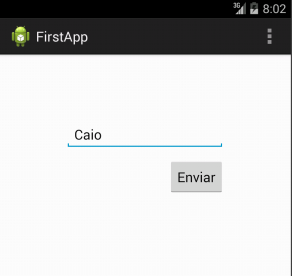
\includegraphics[width=.4\textwidth]{figuras/firstapp/firstapp10.png}
  \caption{Primeira tela após digitar o texto}
  \label{fig:firstapp10}
\end{figure}

\begin{figure}[H]
  \centering
  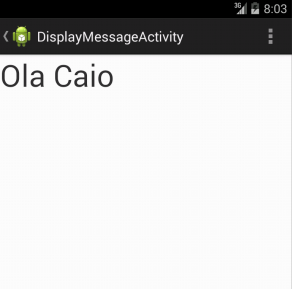
\includegraphics[width=.4\textwidth]{figuras/firstapp/firstapp11.png}
  \caption{Segunda tela mostrando a mensagem enviada}
  \label{fig:firstapp11}
\end{figure}

Para salvar o .apk do aplicativo (atua como instalador do aplicativo para os dispositivos físicos) é só clicar com o direito no projeto pelo \emph{Package Explorer} e em seguida \emph{Export}, por último selecionar a opção \emph{Android/Export Android Application}, são pedidas algumas informações sobre o aplicativo e por fim é gerado o arquivo instalador.

%%%%%%% DESIGN %%%%%%%%%%
\cha{design}{Design}

%%% ACTIVITY %%%
\section{Activity}
Enquanto um usuário navega pelas variadas telas de um aplicativo, sai dele e volta depois, as instâncias de uma \emph{activity} transitam dentre diferentes estados em seu ciclo de vida. Quando um aplicativo é iniciado, uma \emph{activity} inicial é criada o sistema invoca métodos específicos que correspondem a criação dessa \emph{activity}. Durante todo o ciclo de vida vários métodos são chamados, e todos eles correspondem a diferentes estágios desse ciclo de vida. 

Observe na imagem abaixo os métodos correspondentes a cada estado da vida de uma \emph{activity}, quando ela é criada o método \texttt{onCreate()} é o responsável pela configuração inicial. O sistema ao criar uma nova instância de uma \emph{activity}, cada método muda o estado da \emph{activity} um degrau pra cima na pirâmide. 

% COLOCAR FONTE: http://developer.android.com/training/basics/activity-lifecycle/starting.html %
\begin{figure}[H]
  \centering
  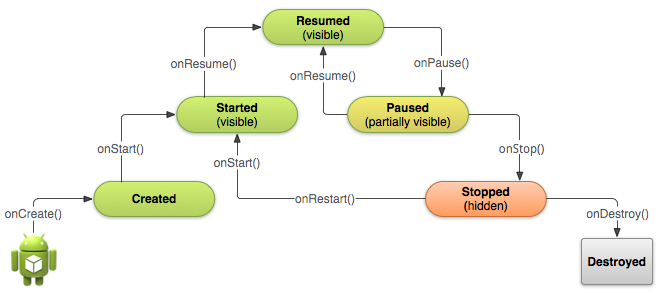
\includegraphics[width=1\textwidth]{figuras/design/basic-lifecycle.png}
  \caption{Ciclo de vida de uma \emph{activity} }
  \label{fig:e2}
\end{figure}

Assim que o usuário começa a sair da \emph{activity}, o sistema invoca outros métodos que movem o estado para níveis mais baixos da pirâmide para começar a desmontar a \emph{activity}. Em alguns casos a \emph{activity} irá apenas ir até certo ponto e esperar (por exemplo quando o usuário troca para outro aplicativo) tal que ela possa voltar de onde parou caso o usuário volte. 

 Não são todos métodos que precisam ser implementados pois isso irá depender da complexidade do seu aplicativo. É importante salientar porém que, implementar esses métodos irá garantir que seu aplicativo se comporte de maneira correta, por exemplo você deve garantir que:
 \bi
 \item Seu aplicativo não falhe quando o usuário receber uma chamada telefônica ou quando o usuário troca de aplicativo;
 \item Seu aplicativo não consuma recursos do sistema enquanto não estiver sendo usado;
 \item Seu aplicativo não perca o progresso do usuário; e
 \item Seu aplicativo não falhe ou perca o progresso do usuário quando a tela rotaciona entre retrato e paisagem.
\ei

Apenas três dentre os estados são estáticos, isto é, a \emph{activity} pode ficar nesse estado por um longo período de tempo:


Retomado \emph{(Resumed)}
	
\hspace*{5mm} Nesse estado a \emph{activity} está em primeiro plano e o usuário pode interagir com ela.
	
Pausado \emph{(Paused)}
	
\hspace*{5mm} Nesse estado a \emph{activity} está parcialmente obscurecida por outra \emph{activity} - a outra \emph{activity} que está em primeiro plano é semi-transparente ou não ocupa todo espaço da tela. A \emph{activity} quando pausada não conseguir interagir com o usuário e não executa nenhum código.
	
Parado \emph{(Stopped)}
	
\hspace*{5mm} Nesse estado a \emph{activity} está completamente oculto e não está visível para o usuário, está em plano de fundo. Quando está parada, uma instância de uma \emph{activity} e toda informação de seu estado tais como variáveis são mantidos, porém a \emph{activity} não executa nenhum código.
	
\section{Especifique a \emph{activity} que inicia seu aplicativo}
\label{sec:especact}

Quando um usuário abre um aplicativo, o sistema chama o método \texttt{onCreate()} da \emph{activity} que foi declarada como sendo a iniciadora do aplicativo. Você pode definir qual \emph{activity} que vai iniciar seu aplicativo no arquivo \texttt{AndroidManifest.xml} que está no diretório raiz do seu projeto.

 A \emph{activity} que inicia seu aplicativo deve ser declarada no manifesto com um \texttt{<intent-filter>}\footnote{Documentação \texttt{<intent-filter>}: \href{http://developer.android.com/guide/topics/manifest/intent-filter-element.html}{http://developer.android.com/guide/topics/manifest/intent-filter-element.html}} que inclui a \texttt{<action>} MAIN e a \texttt{<category>} LAUNCHER. Por exemplo:
 
\begin{listing}[H]
\inputminted[linenos=true,fontsize=\small,frame=lines, framesep=2mm, tabsize=2,numbersep=5pt]{xml}{src/design/launcher-manifest.xml}
\caption{Exemplo de \emph{Launcher activity}}
\end{listing}

%dica
\begin{framed}
\textbf{Dica:} Quando você cria um projeto Android no Eclipse, por padrão é incluída uma classe \emph{activity} que está declarada no manifesto com esse filtro.
\end{framed}

%%% Tipos de Layout %%%
\section{Tipos de \emph{Layout}}
Uma \emph{Activity} contém \emph{Views} e \emph{ViewGroups}. Uma \emph{view} é um elemento que têm presença na tela do dispositivo tais como botões, textos, imagens e etc. Um \emph{ViewGroup} por sua vez é um elemento agrupador de \emph{views} que provê um \emph{layout} na qual você pode ajustar a ordem e aparição das \emph{views}. 

\subsection{LinearLayout}

O \texttt{LinearLayout} arranja \emph{views} em uma única coluna ou uma única linha, desse modo as \emph{views} podem ser arranjadas verticalmente ou horizontalmente. Como mostrado na \autoref{fig:e3}:

\begin{figure}[H]
  \centering
  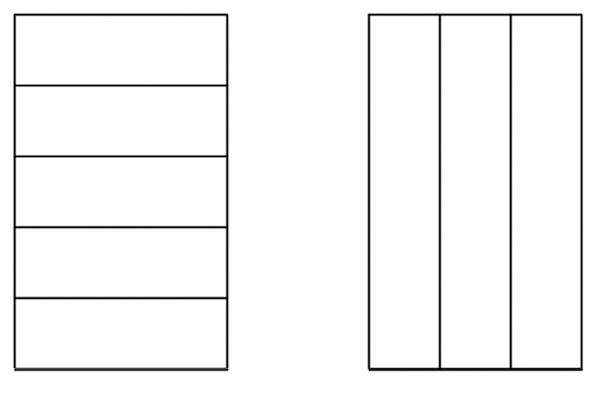
\includegraphics[width=.45\textwidth]{figuras/design/linearlayout.jpg}
  \caption{\texttt{LinearLayout} vertical (à esquerda) e horizontal (à direita)}
  \label{fig:e3}
\end{figure}

\emph{ViewGroups} também podem ser agrupados entre si para a criação de layouts mais complexos, por exemplo é possível agrupar um \texttt{LinearLayout} horizontal dentro de um vertical dessa forma é possível colocar \emph{views} lado a lado em uma camadas do \texttt{LinearLayout} vertical, representada na \autoref{fig:e3}.

\begin{figure}[H]
  \centering
  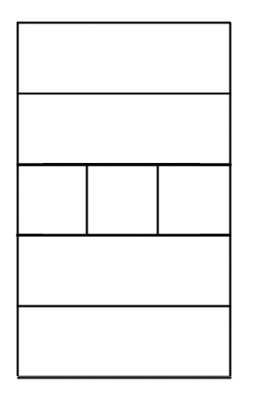
\includegraphics[width=.25\textwidth]{figuras/design/linearlayout-composto.jpg}
  \caption{\texttt{LinearLayout} composto}
  \label{fig:e4}
\end{figure}

\subsection{RelativeLayout}
\label{subsec:relativelayout}

O \texttt{RelativeLayout} permite especificar como as \emph{views} são posicionadas uma em relação a outra. Cada \emph{view} embutida no interior de um \texttt{RelativeLayout} tem atributos que permitem o seu alinhamento com outras \emph{views}. Esses atributos podem ser encontrados na \href{http://developer.android.com/reference/android/widget/RelativeLayout.LayoutParams.html}{documentação}\footnote{ \href{http://developer.android.com/reference/android/widget/RelativeLayout.LayoutParams.html}{http://developer.android.com/reference/android/widget/RelativeLayout.LayoutParams.html}}

\begin{figure}[H]
  \centering
  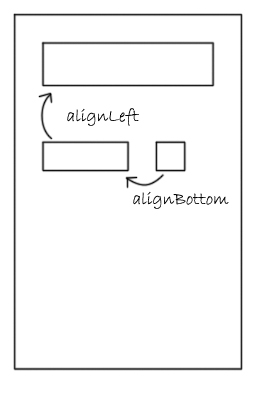
\includegraphics[width=.25\textwidth]{figuras/design/relativelayout.jpg}
  \caption{Exemplo de \texttt{RelativeLayout}}
  \label{fig:e5}
\end{figure}

Novamente cabe comentar que é possível aninhar diferentes \emph{ViewGroups} para formar um \emph{layout} com maior complexidade.

\subsection{FrameLayout}

O \texttt{FrameLayout} é o mais simples e eficiente tipo de \emph{layout}, pode ser usado apenas para mostrar uma \emph{view} ou \emph{views} que se sobrepõem. Geralmente é usado como um recipiente para os \texttt{Fragments}\footnote{Mais informações na seção \ref{sec:frags}}.

Uma \emph{view} definida em um \texttt{FrameLayout} sempre será colocado no canto superior esquerdo da tela do dispositivo ou do \emph{ViewGroup} a que pertence o \texttt{FrameLayout}. Se mais de uma \emph{view} foi definida elas serão empilhadas uma em cima da outra. Isso significa que a primeira \emph{view} adicionada ao \texttt{FrameLayout} será mostrada na base da pilha, e a última adicionada será mostrada no topo.

Você pode fazer com que as \emph{views} não sobreponham as outras usando o atributo \\ \texttt{layout\_gravity}\footnote{\href{http://developer.android.com/reference/android/widget/FrameLayout.LayoutParams.html}{http://developer.android.com/reference/android/widget/FrameLayout.LayoutParams.html}}, dessa forma uma \emph{view} pode ficar posicionada na borda inferior e outra na borda superior e não ficarem sobrepostas.

É possível posicionar as \emph{views} dentro de um \texttt{FrameLayout} usando parâmetros diferentes no \texttt{layout\_gravity}, no exemplo da \autoref{fig:e6} existe um \texttt{FrameLayout} com 3 elementos e cada um com parâmetros diferentes. É possivel combinar os parâmetros utilizando a barra reta '|'.

\begin{figure}[H]
  \centering
  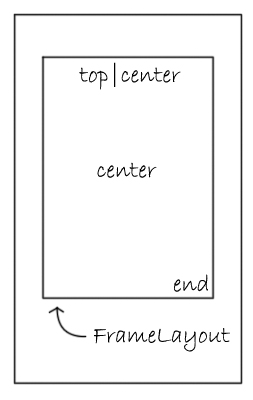
\includegraphics[width=.25\textwidth]{figuras/design/framelayout_gravity.jpg}
  \caption{\texttt{FrameLayout} com exemplo de posicionamento usando \texttt{layout\_gravity}}
  \label{fig:e6}
\end{figure}

\subsection{TableLayout}

\texttt{TableLayouts} podem ser usadas para apresentar dados tabulados ou alinhar conteúdo como tabelas HTML em uma página web. Um \texttt{TableLayout} é composto de \texttt{TableRows}, uma cada para linha da tabela. Os conteúdos das \texttt{TableRows} são as \emph{views} que vão em cada célula da tabela. Cada linha terá zero ou mais células e cada célula pode conter uma \emph{view}. 

O aspecto da \texttt{TableLayout} vai depender de alguns fatores. Primeiro, o número de colunas da tabela inteira vai depender do número de colunas da linha que contém mais colunas. Segundo, a largura de cada coluna é definida como a largura do conteúdo mais largo da coluna. Você pode combinar colunas para formar uma célula maior, mas não pode combinar linhas. Leia mais na \href{http://developer.android.com/reference/android/widget/TableLayout.html}{documentação}\footnote{\href{http://developer.android.com/reference/android/widget/TableLayout.html}{http://developer.android.com/reference/android/widget/TableLayout.html}}

Embora \texttt{TableLayouts} possam ser usados para projetar interfaces, geralmente não é a melhor opção já que são derivadas de \texttt{LinearLayouts}. Se você tem dados que já estão em formato de tabela, como planilhas, então pode ser uma boa opção.

\begin{figure}[H]
  \centering
  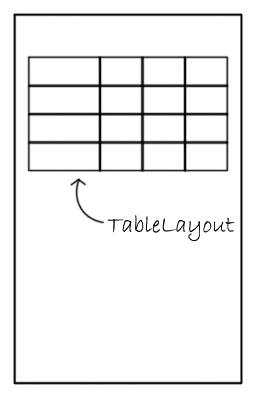
\includegraphics[width=.25\textwidth]{figuras/design/tablelayout.jpg}
  \caption{Exemplo de \texttt{TableLayout}}
  \label{fig:e7}
\end{figure}

%%% LIST VIEW %%%%
\section{Listas \texttt{(ListView)}}\footnote{Documentação \texttt{ListView}:\href{http://developer.android.com/reference/android/widget/ListView.html}{http://developer.android.com/reference/android/widget/ListView.html}}
Listas são uma das formas mais simples e poderosas de se mostrar informações ao usuário de forma objetiva. A \texttt{ListView} é capaz de aprensentar uma lista rolável de itens. 

\begin{figure}[H]
  \centering
  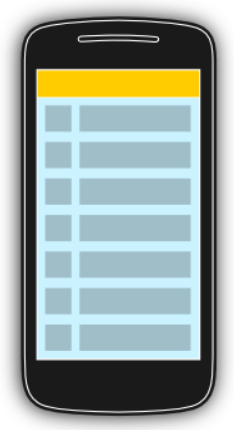
\includegraphics[width=.25\textwidth]{figuras/design/listview-scheme.png}
  \caption{Esquema de uma lista}
  \label{fig:e8}
\end{figure}

Um item individual da lista pode ser selecionado, essa seleção pode acionar uma outra tela com detalhes do item.


\begin{figure}[H]
  \centering
  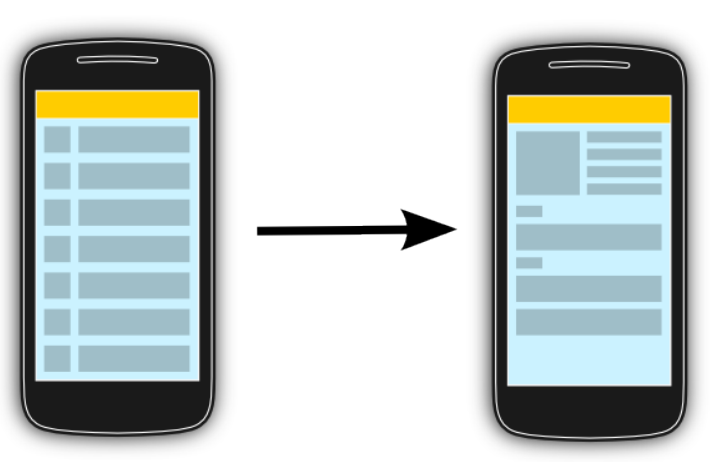
\includegraphics[width=.45\textwidth]{figuras/design/listview-scheme2.png}
  \caption{Detalhes de um elemento da lista}
  \label{fig:e9}
\end{figure}

\subsection{Adaptadores}
	Adaptadores são usados para providenciar dados a \emph{views}. O adaptador também define como item da \emph{view} será mostrada. Para \texttt{ListViews} o adaptador define como cada linha será mostrada.
	
	Um adaptador deve estender a classe base \texttt{BaseAdapter}. O Android já tem alguns adaptadores padrão, os mais importantes são o \texttt{ArrayAdapter} e o \texttt{CursorAdapter}. 
	
	O \texttt{ArrayAdapter} é usado para manipular dados em \emph{arrays} ou listas (\texttt{java.util.List}). Já o \texttt{SimpleCursorAdapter} consegue manipular dados em banco de dados.

\subsection{Construção}

A construção desse tipo de design é simples. No arquivo de \emph{layout} da \emph{activity} use o \texttt{LinearLayout} para conter a \texttt{ListView}.

\begin{listing}[H]
\inputminted[linenos=true,fontsize=\small,frame=lines, framesep=2mm, tabsize=2,numbersep=5pt]{xml}{src/design/layout_linear.xml}
\caption{\texttt{LinearLayout} no arquivo de \emph{layout}}
\label{code:linearlayout}
\end{listing}

Se estiver usando o construtor de interface gráfica, pode arrastar uma \texttt{ListView} para dentro do \emph{layout}. Caso contrário pode construir manualmente no arquivo XML do \emph{layout} da \emph{activity}. 

Você deve colocar o \texttt{LinearLayout} como raiz do arquivo XML, o elemento raiz sempre deve conter o atributo \texttt{xmlns:android} como mostrado na linha 2 do \hyperref[code:linearlayout]{Algoritmo \ref*{code:linearlayout}}, não entraremos em detalhes sobre os outros atributos. 

Adicione uma \texttt{ListView}, escreva o código abaixo dentro do \texttt{LinearLayout}. 
\begin{listing}[H]
\inputminted[linenos=true,fontsize=\small,frame=lines, framesep=2mm, tabsize=2,numbersep=5pt]{xml}{src/design/listview.xml}
\caption{Código de uma \texttt{ListView}}
\end{listing}

Você precisa popular a lista, para isso você pode criar um \texttt{string-array} no arquivo \texttt{strings.xml} com os elementos que deseja colocar na lista. Nesse exemplo do \hyperref[code:string-array]{Algoritmo \ref*{code:string-array}} foi criado uma lista com nome \texttt{listString} e 4 itens que serão mostrados em forma de lista pela \texttt{ListView}.

\begin{listing}[H]
\inputminted[linenos=true,fontsize=\small,frame=lines, framesep=2mm, tabsize=2,numbersep=5pt]{xml}{src/design/string-array.xml}
\caption{\texttt{string-array} populada com elementos}
\label{code:string-array}
\end{listing}

Finalmente, você deve escrever o código que irá preencher a lista com as \emph{strings}. Como é feito no \hyperref[code:activity-lista]{Algoritmo \ref*{code:activity-lista}}.

\begin{listing}[H]
\inputminted[linenos=true,fontsize=\small,frame=lines, framesep=2mm, tabsize=2,numbersep=5pt]{java}{src/design/listactivity.java}
\caption{Código de uma \emph{activity} com lista clicável}
\label{code:activity-lista}
\end{listing}

Primeiro, na linha 2, foi criada uma variável do tipo \texttt{ListView} para guardar um ponteiro para a \emph{view} já definida no \emph{layout}.

No método \texttt{onCreate()} você precisa criar e inicializar a lista na sua \emph{activity}. Na linha 10 obtemos as \emph{strings} do \texttt{string-array} e o guardamos na variável \texttt{listStr}. Usamos o método \texttt{getResources()} para poder adquirir o ponteiro para os recursos do aplicativo. Na linha 13 conseguimos o ponteiro pra lista e o guardamos na variável criada.

Usamos o adaptador ao chamar o método \texttt{ListView.setAdapter()} nas linhas 16-17  e passamos como parâmetro a criação de um novo adaptador do tipo \texttt{ArrayAdapter}. Para o construtor\footnote{\href{http://developer.android.com/reference/android/widget/ArrayAdapter.html}{http://developer.android.com/reference/android/widget/ArrayAdapter.html}} desse adaptador está sendo passado o contexto atual da \emph{activity}, um \emph{layout} pré-definido do sistema, o \texttt{simple\_list\_item\_1}, e os dados na forma de \emph{array}.

Na linha 22 usamos o método \texttt{ListView.setOnItemClickListener} para configurar uma ação a ser executada quando um item da lista for clicado. Neste exemplo é criado um \texttt{Toast}, o \texttt{Toast} mostra uma mensagem em uma caixa de texto na parte inferior da tela por um curto período de tempo, nesse caso irá mostrar o mesmo texto do item da lista que foi clicado. Uma das aplicações mais comuns é fazer com que ao se clicar em um item da lista, uma nova \emph{activity} seja aberta com detalhes do item.

\begin{figure}[H]
  \centering
  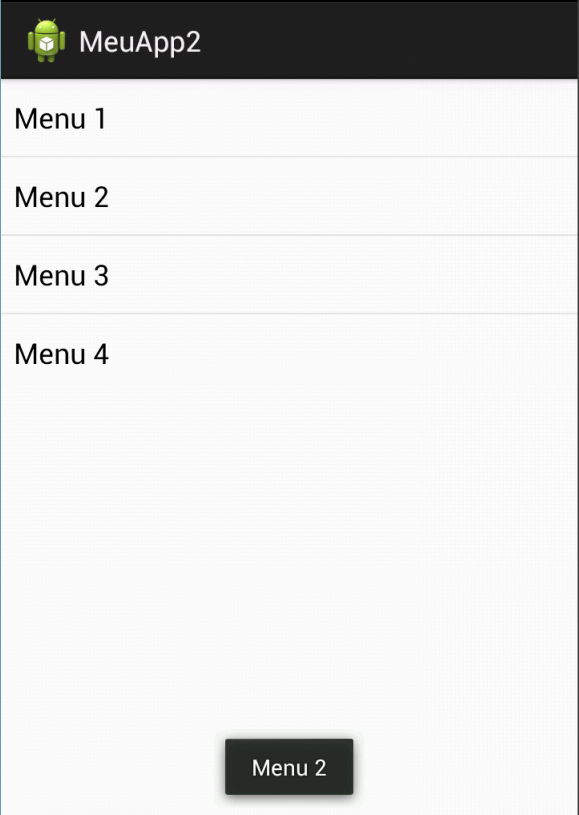
\includegraphics[width=.4\textwidth]{figuras/design/lista.png}
  \caption{Lista simples}
  \label{fig:e10}
\end{figure}

A \autoref{fig:e10} mostra como ficou o exemplo ao ser executado em um \emph{smartphone}, o item ''Menu 2'' foi clicado e um \texttt{Toast} foi mostrado no momento do clique.

%%% LIST ADAPTER %%%
\section{Listas Compostas}
É possível compor um item da lista colocando mais elementos além de um texto. Para isso você precisa criar um novo arquivo XML que irá definir a customização de cada linha da \texttt{ListView}, nesse exemplo iremos definir um arquivo chamado \texttt{item.xml}, mostrado abaixo.


\begin{listing}[H]
\inputminted[linenos=true,fontsize=\small,frame=lines, framesep=2mm, tabsize=2,numbersep=5pt]{xml}{src/design/item.xml}
\caption{Código do arquivo \texttt{item.xml}}
\label{code:itemxml}
\end{listing}	

O \hyperref[code:itemxml]{Algoritmo \ref*{code:itemxml}} mostra como você pode fazer a customização de um item da lista. Nesse exemplo há uma pequena imagem à esquerda e dois textos de cores e tamanhos diferentes. 
Para isso primeiro criamos um \texttt{LinearLayout} que irá conter uma \texttt{ImageView} para mostrar a imagem e outro \texttt{LinearLayout} para colocar os dois textos. As cores do textos são configuradas com o atributo \texttt{textColor} e usa o padrão HTML de cores.

Agora você precisa usar um adaptador para mostrar esse layout customizado em cada linha da lista, usaremos a classe \texttt{SimpleAdapter}\footnote{\href{http://developer.android.com/reference/android/widget/SimpleAdapter.html}{http://developer.android.com/reference/android/widget/SimpleAdapter.html}}. Essa classe faz a adaptação de um \texttt{ArrayList} de \texttt{Maps} para um \emph{layout} definido. 

\begin{listing}[H]
\inputminted[linenos=true,fontsize=\small,frame=lines, framesep=2mm, tabsize=2,numbersep=5pt]{java}{src/design/customlist.java}
\caption{Código da lista customizada}
\label{code:custom-list}
\end{listing}	

Observando o \hyperref[code:custom-list]{Algoritmo \ref*{code:custom-list}}. Na linha 13 criamos um \texttt{ArrayList} de \texttt{Maps}. Na linha 14 e 19 criamos um \texttt{HashMap} onde a chave é uma \emph{string} que identifica o conteúdo, essas chaves serão \emph{userIcon}, \emph{userName} e \emph{userText} respectivamente. Em \emph{userIcon} colocamos uma imagem, essa imagem deve ser colocada nas subpastas da pasta \texttt{drawable} e é acessada através da classe \texttt{R}. Em \emph{userName} colocamos um nome de usuário, por exemplo. Em \emph{userText} poderia ser colocada uma descrição, ou uma frase customizada do usuário mas nesse exemplo foi colocado uma sentença qualquer. Nas linhas 18 e 23 adicionamos o \texttt{Map} criado no \texttt{ArrayList}.

Criamos o \texttt{SimpleAdapter} nas linhas 26-29. Para o construtor passamos o \texttt{ArrayList} de \texttt{Maps} que contém os dados, passamos também o \emph{layout} que definimos anteriormente \\ \texttt{R.layout.item}. Passamos um \emph{array} de \emph{strings} que contém as chaves que serão usadas para obter os dados e por último um \emph{array} de inteiros que contém os \emph{ids} das \emph{views} em que os conteúdos dos \texttt{Maps} serão colocados.

\begin{figure}[H]
  \centering
  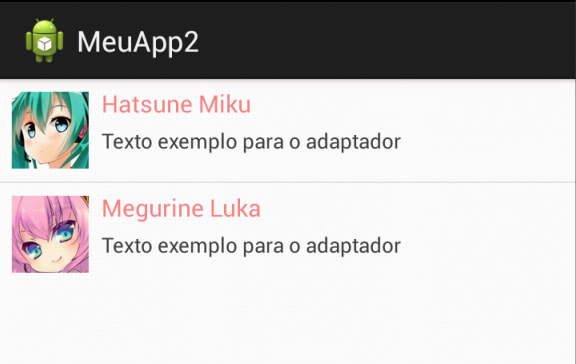
\includegraphics[width=.475\textwidth]{figuras/design/lista-composta.png}
  \caption{Lista Composta}
  \label{fig:e11}
\end{figure}

A \autoref{fig:e11} mostra como ficou o exemplo acima ao ser executado em um \emph{smartphone}. 

%%% EXPANDABLE LIST %%%
\section{Listas expansíveis \texttt{(ExpandableListView)}}

Listas expansíveis são úteis para agrupar conjuntos de itens semelhantes, funcionam da mesma maneira que as listas comuns e podem ser customizadas.
Comece colocando sua lista no \emph{layout} da \emph{activity} desejada.
	
\begin{listing}[H]
\inputminted[linenos=true,fontsize=\small,frame=lines, framesep=2mm, tabsize=2,numbersep=5pt]{xml}{src/design/exlist.xml}
\caption{Código XML de uma Lista expansível}
\end{listing}	

\begin{framed}
\textbf{Dica:} O atributo \texttt{transcriptMode=''alwaysScroll''} vai fazer com que a lista sempre role até o final quando você expande ou contrai um grupo.
O atrbuto \texttt{listSelector} colore o item da lista quando este é clicado.
\end{framed}

Agora crie 2 novos arquivos XML, um chamado \texttt{list\_item\_parent.xml} e o outro chamado \texttt{list\_item\_child.xml} dentro da pasta \texttt{res/layout}.

\begin{listing}[H]
\inputminted[linenos=true,fontsize=\small,frame=lines, framesep=2mm, tabsize=2,numbersep=5pt]{xml}{src/design/list-item-parent.xml}
\caption{Layout \texttt{list\_item\_parent.xml}}
\end{listing}	

Nesses dois \emph{layouts} teremos apenas uma \texttt{TextView} para abrigar um texto.

\begin{listing}[H]
\inputminted[linenos=true,fontsize=\small,frame=lines, framesep=2mm, tabsize=2,numbersep=5pt]{xml}{src/design/list-item-child.xml}
\caption{Layout \texttt{list\_item\_child.xml}}
\end{listing}	

Em seguida precisamos criar uma classe que irá abrigar os dados dos elementos pai, elementos estes que serão expandidos quando clicados. Nesse exemplo criamos uma classe \emph{Parent}, como mostrado no \hyperref[code:parent]{Algoritmo \ref*{code:parent}}.

\begin{listing}[H]
\inputminted[linenos=true,fontsize=\small,frame=lines, framesep=2mm, tabsize=2,numbersep=5pt]{java}{src/design/parent.java}
\caption{Classe \texttt{Parent}}
\label{code:parent}
\end{listing}	

Essa classe contém o texto do item, que será guardado na \emph{string} \texttt{mTitle} e um \texttt{ArrayList} que irá comportar os sub-itens desse item. Os métodos \emph{get} e \emph{set} são simples.

Em seguida, crie uma nova classe, \texttt{CustomAdapter} que será o adaptador da lista expansível para os dados, para esse exemplo estaremos adaptando apenas para o uso de texto. Essa classe deve estender a classe \texttt{BaseExpandableListAdapter}.

\newenvironment{code}{\captionsetup{type=listing}}{}

\begin{code}
\inputminted[linenos=true,fontsize=\small,frame=lines, framesep=2mm, tabsize=2,numbersep=5pt]{java}{src/design/customadapter.java}
\caption{Classe \texttt{CustomAdapter}}
\end{code}

% problema com paragrafo
\parskip 1pt 

Primeiro precisamos de um \texttt{LayoutInflater}\footnote{\href{http://developer.android.com/reference/android/view/LayoutInflater.html}{http://developer.android.com/reference/android/view/LayoutInflater.html}} que irá instanciar o \emph{layout} XML nas \emph{views} correspondentes, e um \emph{array} da classe \texttt{Parents} que criamos anteriormente, esses serão os itens principais da lista.

Na linha 7 no construtor da classe, usamos o método \texttt{LayoutInflater.from()} para obter o \emph{inflater} do contexto da \emph{activity}. 

Ao estender a classe \texttt{BaseExpandableListAdapter} temos que programar alguns métodos. O método \texttt{getChild()} deve adquirir o ponteiro para um subitem de um item na lista. O método \texttt{getChildId()} deve obter o \emph{id} de um subitem, porém nesse exemplo não temos nada configurado então usamos a própria posição desse subitem como \emph{id} e retornamos \texttt{childPosition}. 

O método \texttt{getChildView} na linha 24 vai atribuir o \emph{layout} dos subitens na linha 28. Na linha 32 obtemos o \texttt{TextView} desse subitem e com o método \texttt{TextView.setText()} atribuímos seu respectivo texto. Esse texto está guardado no \emph{array} chamado \texttt{mArrayChildren} da classe \texttt{Parent}, então a fim de obter esse texto devemos obter o \texttt{Parent} correto. Quando você clica em um item da lista, o Android guarda qual item você clicou no parâmetro \texttt{groupPosition}. Em seguida se obtém o texto de cada subitem pelo parâmetro \texttt{childPosition}.

Outro método importante é o \texttt{getGroupView}, funciona da mesma maneira que \texttt{getChildView} mas configurando os \emph{views} dos itens pai em vez dos subitens.

Para finalizar, você deve construir os objetos na classe da \emph{activity}, nesse exemplo para popular a lista eu coloquei no arquivo de \texttt{strings} alguns fabricantes e modelos de carros, você pode obtê-los no repositório do projeto.

\begin{listing}[H]
\inputminted[linenos=true,fontsize=\small,frame=lines, framesep=2mm, tabsize=2,numbersep=5pt]{java}{src/design/exlist-main.java}
\caption{Construindo a lista expansível na \emph{activity}}
\label{code:listaexp-ac}
\end{listing}	

\newpage

O \hyperref[code:listaexp-ac]{Algoritmo \ref*{code:listaexp-ac}} é a construção da lista expansível na \emph{activity}, na linha 9-10 obtemos a \emph{view} usando \texttt{findViewById()}. A linha 30-31 são um pouco mais complicadas, primeiro é preciso obter o \emph{id} do \texttt{string-array} que é subitem do item atual no laço de repetição. Para isso usamos \texttt{getResources().getIdentifier()} para obter o \emph{id} do subitem a partir do nome do item pai. Em seguida podemos acessar o \texttt{string-array} normalmente como é feito na linha 31.

 Na linha 41 usamos o \texttt{CustomAdapter} que criamos anteriormente.

\begin{figure}[H]
  \centering
  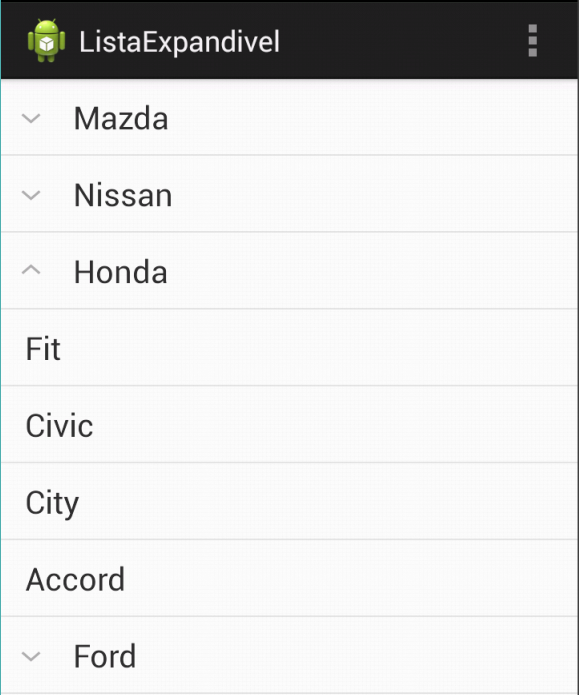
\includegraphics[width=.475\textwidth]{figuras/design/listaexpandivel.png}
  \caption{Exemplo de lista expansível rodando em um \emph{smartphone}}
  \label{fig:e12}
\end{figure}

%%% GRADES E IMAGENS %%%
\newpage
\section{Grades \texttt{(GridView)} e imagens \texttt{ImageView}}

Grades são úteis para mostrar imagens e fotos como uma galeria, ou permitir a seleção de categorias semelhante a uma lista. A idéia é ter elementos lado a lado para mostrar ou para selecionar e mostrar mais detalhes. Basicamente funciona como uma grade bi-dimensional que pode ser arrastada para os lados ou de cima pra baixo. 

\begin{figure}[H]
  \centering
  
\includegraphics[width=.475\textwidth]{figuras/design/gridview.png}
  \caption{Esquema de um \texttt{GridView}}
  \label{fig:e14}
\end{figure}

Comece colocando um \texttt{GridView}\footnote{\href{http://developer.android.com/reference/android/widget/GridView.html}{http://developer.android.com/reference/android/widget/GridView.html}} no \emph{layout} de sua \emph{activity}.

\begin{listing}[H]
\inputminted[linenos=true,fontsize=\small,frame=lines, framesep=2mm, tabsize=2,numbersep=5pt]{xml}{src/design/gridview.xml}
\caption{Layout do \texttt{GridView}}
\end{listing}	

Vamos criar uma nova classe que será o adaptador de imagens para o \texttt{GridView}, chamemos a classe de \texttt{ImageAdapter}, ela é mostrada no \hyperref[code:image-adapter]{Algoritmo \ref*{code:image-adapter}}.

\begin{listing}[H]
\inputminted[linenos=true,fontsize=\small,frame=lines, framesep=2mm, tabsize=2,numbersep=5pt]{java}{src/design/imageadapter.java}
\caption{Classe \texttt{ImageAdapter}}
\label{code:image-adapter}
\end{listing}	

A classe \texttt{ImageAdapter} deve ser subclasse da classe \texttt{BaseAdapter}\footnote{\href{http://developer.android.com/reference/android/widget/BaseAdaptfer.html}{http://developer.android.com/reference/android/widget/BaseAdapter.html}}. Temos, como variável pública, um \emph{array} das imagens que queremos colocar na grade. Como todo \emph{id} de um recurso da classe \texttt{R} é um inteiro, criamos um \emph{array} de inteiros. Note que estamos considerando que todas as imagens já foram devidamente colocadas na pasta \texttt{drawable}.

O método mais importante é o método \texttt{getView()}. Nele criamos uma nova \texttt{ImageView}\footnote{\href{http://developer.android.com/reference/android/widget/ImageView.html}{http://developer.android.com/reference/android/widget/ImageView.html}} para abrigar a imagem que queremos colocar na grade. Em seguida configuramos alguns parâmetros desse \texttt{ImageView}, o método \texttt{ImageView.setImageResource()} é responsável por estabelecer um \texttt{drawable} como conteúdo do \texttt{ImageView}. \\ Já o método \texttt{View.setLayoutParams()} configura os parâmetros de \emph{layout} associados com essa \emph{view}, note que para esse método passamos parâmetros de \emph{layout} de uma \texttt{GridView}, que por sua vez recebe \texttt{(200,200)} como largura e altura de um elemento da grade.

  \texttt{ImageView.setScaleType} controla como a imagem deve ser redimensionada para condizer com o tamanho do \texttt{ImageView}, \texttt{ImageView.ScaleType}\footnote{\href{http://developer.android.com/reference/android/widget/ImageView.ScaleType.html}{http://developer.android.com/reference/android/widget/ImageView.ScaleType.html}} são as formas disponíveis para escalar a imagem.

Agora basta criar a grade em sua \emph{activity}.

\begin{listing}[H]
\inputminted[linenos=true,fontsize=\small,frame=lines, framesep=2mm, tabsize=2,numbersep=5pt]{java}{src/design/grade-activity.java}
\caption{\emph{activity} com grade}
\end{listing}	

Exemplo acima rodando em um \emph{smartphone} na \autoref{fig:e15}:

\begin{figure}[H]
  \centering
  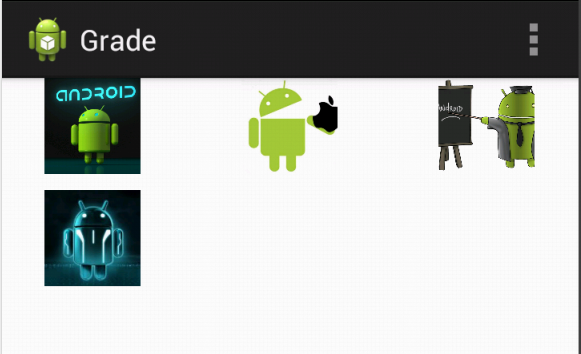
\includegraphics[width=.475\textwidth]{figuras/design/grade-exemplo1.png}
  \caption{Demonstração de um \texttt{GridView}}
  \label{fig:e15}
\end{figure}

Para complementar, você pode fazer com que a imagem abra em tela cheia quando clicada na view, para isso é necessário que você passe o \emph{id} do recurso do \texttt{GridView} para uma nova \emph{activity} que irá mostrar a imagem em tela cheia.
Para isso precisamos criar um novo \emph{layout} XML, a qual chamaremos de \texttt{full\_image.xml}, nele teremos apenas uma \texttt{ImageView} e um \texttt{TextView} que será uma pequena legenda da imagem.

\begin{listing}[H]
\inputminted[linenos=true,fontsize=\small,frame=lines, framesep=2mm, tabsize=2,numbersep=5pt]{xml}{src/design/full-image.xml}
\caption{Layout \texttt{full\_image.xml}}
\end{listing}	

Note que para o \texttt{TextView} usaremos o atributo \texttt{layout\_width} como \texttt{fill\_parent} e \texttt{layout\_height} como \texttt{40dp}, dessa forma criamos um pequeno retângulo de altura fixa mas de forma que a largura preencha a tela completamente. O atributo \texttt{background} com o valor \texttt{\#55555555} faz com que a cor do retângulo seja cinza com transparência, já que o parâmetro \emph{alfa} também tem valor 0x55. Também deixamos o texto com cor branca com o atributo \texttt{textColor}.

Em seguida, crie uma nova classe chamada \texttt{FullImageActivity}, essa é a \emph{activity} que vai mostrar a imagem em tela cheia. A construção da classe é simples, você deve apenas obter o \emph{id} da imagem passado como \emph{extra} através do \texttt{intent} e então obter essa imagem da classe \texttt{ImageAdapter}.

\begin{listing}[H]
\inputminted[linenos=true,fontsize=\small,frame=lines, framesep=2mm, tabsize=2,numbersep=5pt]{java}{src/design/FullImageActivity.java}
\caption{Classe \texttt{FullImageActivity}}
\end{listing}	 	 	

\begin{listing}[H]
\inputminted[linenos=true,fontsize=\small,frame=lines, framesep=2mm, tabsize=2,numbersep=5pt]{java}{src/design/grid-activity-p2.java}
\caption{Código da \emph{activity} após as modificações}
\label{code:act-fullimage}
\end{listing}	 

No \hyperref[code:act-fullimage]{Algoritmo \ref*{code:act-fullimage}}, configuramos um \texttt{View.setOnItemClickListener()} de forma que quando uma imagem da grade for clicada, um \texttt{Intent} seja enviado a uma nova \emph{activity} que por sua vez ficará encarregada de mostrar a imagem em tela cheia.  Quando um item é clicado conseguimos obter a posição dele na grade com o parâmetro \texttt{pos} da função \texttt{onItemClick()}, essa posição é equivalente ao \emph{id} da imagem no \emph{array} criado na classe \texttt{ImageAdapter}.  A \texttt{FullImageActivity} por sua vez recebe esse \texttt{Intent} que possui o \emph{id} da imagem que deve ser mostrada e configura o \texttt{ImageView} de acordo. 

\begin{figure}[H]
  \centering
  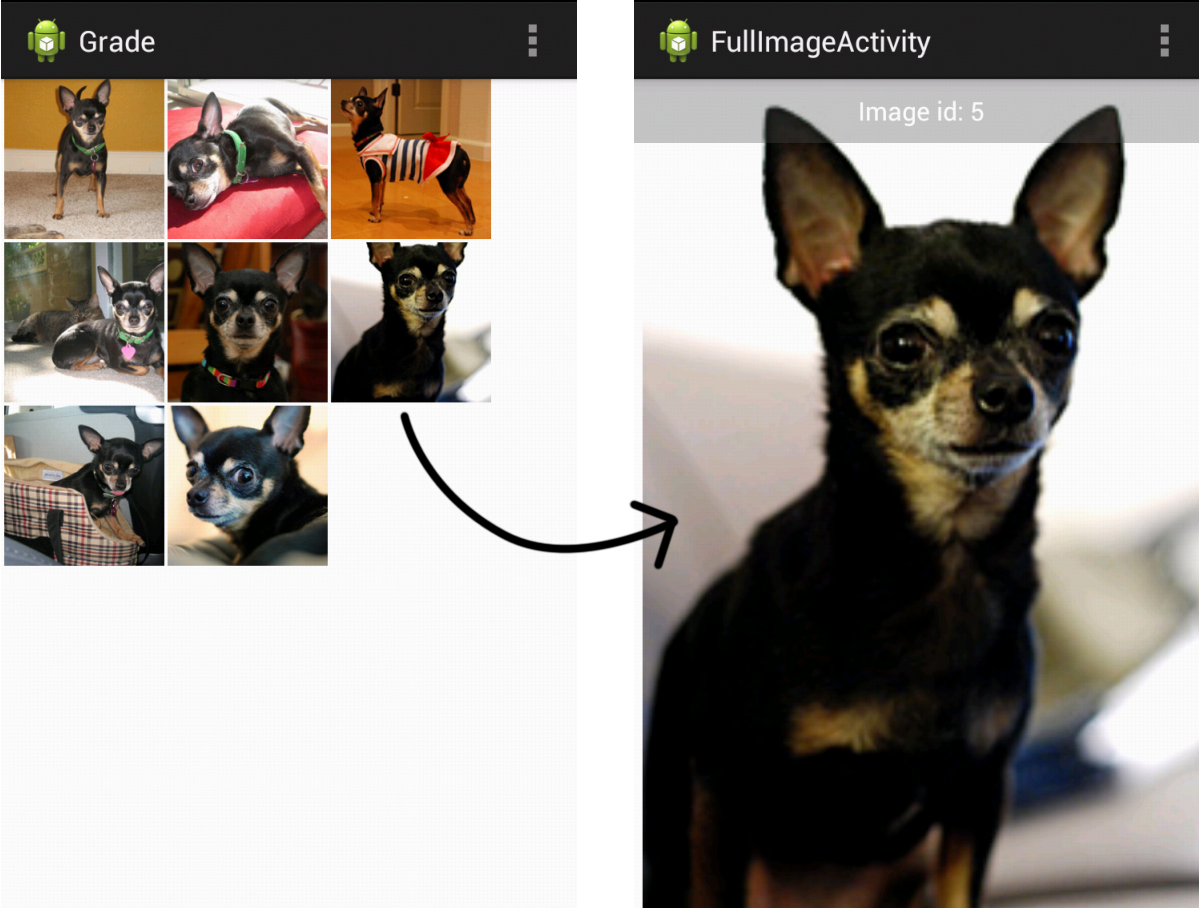
\includegraphics[width=.80\textwidth]{figuras/design/grid-fullimage.jpg}
  \caption{Exemplo \texttt{GridView} com imagem em tela cheia}
  \label{fig:e16}
\end{figure}

%% FRAGMENTOS %%
\section{Fragmentos}
\label{sec:frags}

Fragmentos são a solução do Android para criar interfaces de usuário modulares, eles vivem dentro das \emph{activity} e uma \emph{activity} pode conter vários fragmentos. Assim como as \emph{activity} os fragmentos possuem um ciclo de vida. %% EXPLICAR MELHOR %%.

Dentre as vantagens de um fragmento estão:
\bi
	\item Modularidade e reúso de código;
	\item Habilidade de construir interfaces com múltiplos painéis;
	\item Facilidade de construir aplicativos para celulares e tablets.
\ei

O primeiro conceito a ser coberto é como construir um fragmento, comece definindo o \emph{layout} do fragmento.

Um layout bem simples, apenas com um botão para efeito de demonstração. Agora crie uma classe \texttt{BasicFragment}

\begin{listing}[H]
\inputminted[linenos=true,fontsize=\small,frame=lines, framesep=2mm, tabsize=2,numbersep=5pt]{java}{src/design/basicfragment.java}
\caption{Classe \texttt{BasicFragment}}
\end{listing}	

Caso você esteja desenvolvendo para API menores que 11 (HoneyComb 3.0) você vai precisar usar a API de retrocompatibilidade que o Google providenciou para essas APIs, você precisa importar a classe de suporte: \mint{java}|import android.support.v4.app.Fragment;|

%% diferença chave? %%
% One of the key differences between a Fragment and an Activity is that Fragments instantiate their Views inside the onCreateView() callback and Activities instantiate their Views using the setContentView() method inside of the onCreate() callback. Fragments also have to manually instantiate their Views using an instance of LayoutInflater, which is provided to the onCreateView() method for convenience. %%

%% Another difference is that a Fragment is not a subclass of Context. This means that a Fragment can not be launched as a component inside your app and therefore always has to live inside of an Activity. This also means that whenever you need a Context inside of a Fragment, you need to get access to the parent Activity. You can do this by using the getActivity() method as we have done in the Fragment button's OnClickListener callback. You need to watch out because getActivity() can return null depending on where the Fragment is in the Activity's lifecycle. So, you should also include a check to see if the Activity is null before you use it. %%

Agora para incluir o fragmento na \emph{activity} existem duas opções. A primeira é inlcluir o fragmento no XML da \emph{activity} como você faria com qualquer \texttt{view}.

\begin{listing}[H]
\inputminted[linenos=true,fontsize=\small,frame=lines, framesep=2mm, tabsize=2,numbersep=5pt]{xml}{src/design/fragment-activity.xml}
\caption{Layout da \emph{activity} com um fragmento}
\end{listing}	

Você pode usar o \texttt{<fragment>} quantas vezes quiser para incluir múltiplos fragmentos.
Note que você precisa usar um nome qualificado em \texttt{android:name}, veja mais na documentação oficial: \href{http://developer.android.com/guide/topics/manifest/activity-element.html\#nm}{activity-element}\footnote{\href{http://developer.android.com/guide/topics/manifest/activity-element.html\#nm}{http://developer.android.com/guide/topics/manifest/activity-element.html\#nm}}

Novamente, caso esteja desenvolvendo para APIs menores que 11, você vai precisar fazer a \emph{activity} estender a classe \texttt{FragmentActivity} e importar a classe de suporte: \mint{java}|import android.support.v4.app.FragmentActivity;|
\mint{java}|public class MainActivity extends FragmentActivity|


Simplesmente configurando a \emph{activity} para usar o fragmento vai fazer com que o fragmento seja adicionado e renderizado na tela, entretanto você deve querer ter mais controle de quando e como seus fragmentos serão adicionados durante o curso do seu aplicativo. Para isso existe uma maneira alternativa de adicionar o fragmento em tempo de execução. A fim de adicionar o fragmento em tempo de execução você precisa fazer uma mudança no layout da \emph{activity}:

\begin{listing}[H]
\inputminted[linenos=true,fontsize=\small,frame=lines, framesep=2mm, tabsize=2,numbersep=5pt]{xml}{src/design/framelayout.xml}
\caption{Layout da \emph{activity} com o \texttt{FrameLayout}}
\end{listing}	

E uma mudança na \emph{activity} que vai mostrar o fragmento:

\begin{listing}[H]
\inputminted[linenos=true,fontsize=\small,frame=lines, framesep=2mm, tabsize=2,numbersep=5pt]{java}{src/design/activity-frag-dyn.java}
\caption{\emph{activity} com adição dinâmica de fragmento}
\end{listing}	

E dessa forma obtemos o mesmo resultado, porém com a adição dinâmica do fragmento, você pode experimentar e fazer com que o botão remova um fragmento e coloca outro diferente no lugar.

%% TABS %%

\section{Abas (\emph{Tabs})}
	Existem diversas maneiras de criar uma interface com abas no Android, uma delas é usando as interfaces \texttt{TabHost} e \texttt{TabWidget}, outra é imitando o comportamento usando apenas \texttt{Fragments}. 

	%% TABHOST TABWIDGET %%	
	\subsection{Usando \texttt{TabHost} e \texttt{TabWidget}}
	
	Abas usando essas interfaces são suportadas por todas as versões do Android.Vamos criar uma interface com abas seguindo esse esquema:
	
	\begin{figure}[H]
	  \centering
	  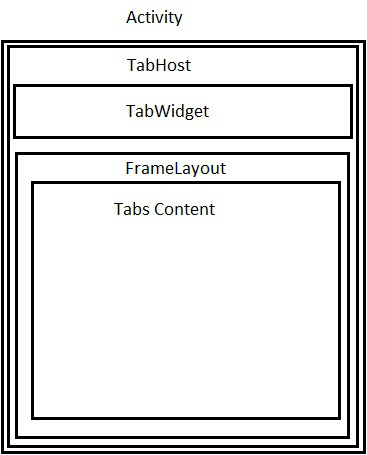
\includegraphics[width=.275\textwidth]{figuras/design/tabs1.jpg}
	  \caption{Esquema da interface com abas}
	  \label{fig:e17}
	\end{figure}
	
	Primeiro precisamos criar uma \emph{activity} que servirá como recipiente para as abas e seu conteúdo. O \texttt{TabWidget}\footnote{\href{http://developer.android.com/reference/android/widget/TabWidget.html}{http://developer.android.com/reference/android/widget/TabWidget.html}} é o controle de seleção das abas. Todo conteúdo das abas ficará contido dentro do \texttt{FrameLayout}, é nele que as respectivas \emph{activities} serão mostradas. O \texttt{TabHost}\footnote{\href{http://developer.android.com/reference/android/widget/TabHost.html}{http://developer.android.com/reference/android/widget/TabHost.html}} por sua vez serve como um recipiente para o \texttt{TabWidget} e o \texttt{FrameLayout}.
	
	Crie um novo projeto com nome \texttt{TabHostRelativeLayout} e nomeie a \emph{activity} como \texttt{TabLayoutActivity}. No XML que define o \emph{layout} da \emph{activity}, insira o \texttt{TabHost}, o \texttt{TabWidget} e \texttt{FrameLayout} como mostrado no \hyperref[code:layout-tabhost]{Algoritmo \ref*{code:layout-tabhost}}.
	
	\begin{listing}[H]
	\inputminted[linenos=true,fontsize=\small,frame=lines, framesep=2mm, tabsize=2,numbersep=5pt]{xml}{src/design/activity-tab-host.xml}
	\caption{\emph{Layout} da \emph{activity} \texttt{TabHostLayout}}
	\label{code:layout-tabhost}
	\end{listing}
	
	Precisamos criar 3 novas \texttt{Activitys} que serão os fragmentos (telas) exibidos, para fazer isso navegue pelo \texttt{Package Explorer} \texttt{TabHostRelativeLayout->src} e clique com o botão direito em \texttt{com.example.tabhostrelativelayout} e em seguida \texttt{new->other}, selecione \texttt{Android->Android Activity} e selecione como \emph{Empty Activity}, a primeira terá \emph{Activiry Name} de \emph{Tab1Fragment}, a segunda  \emph{Tab2Fragment} e a terceira  \emph{Tab3Fragment}.
	
	Agora precisamos definir o \emph{layout} dos fragmentos, isto é, o \emph{layout} de cada aba. Para simplificar o exemplo, as abas só terão um fundo colorido, de cores diferentes. Para isso usa-se o atributo \texttt{background}. Os arquivos que devem ser editados são: \texttt{TabHostRelativeLayout->res->} \texttt{->layout->activity\_tab1\_fragment.xml} assim como \texttt{activity\_tab2\_fragment.xml} e \texttt{activity\_tab3\_fragment.xml}.
	
	\begin{listing}[H]
	\inputminted[linenos=true,fontsize=\small,frame=lines, framesep=2mm, tabsize=2,numbersep=5pt]{xml}{src/design/tab-fragment.xml}
	\caption{\emph{tab\_fragment1.xml}}
	\end{listing}
	
	\begin{listing}[H]
	\inputminted[linenos=true,fontsize=\small,frame=lines, framesep=2mm, tabsize=2,numbersep=5pt]{xml}{src/design/tab-fragment2.xml}
	\caption{\emph{tab\_fragment2.xml}}
	\end{listing}
		
	\begin{listing}[H]
	\inputminted[linenos=true,fontsize=\small,frame=lines, framesep=2mm, tabsize=2,numbersep=5pt]{xml}{src/design/tab-fragment3.xml}
	\caption{\emph{tab\_fragment3.xml}}
	\end{listing}
	
	Quando um bloco é declarado como \texttt{Linear Layout} os elementos são adicionados em sequência na tela (se colocar duas caixas de texto, elas ficarão uma ao lado da outra, não será possível posicionar da maneira que desejar), isso pode ser utilizado em uma página com um longo texto por exemplo (quando exceder o tamanho da tela é criado um \emph{scroll bar}). Nesse caso como uma estrutura de abas precisamos declarar como \texttt{Linear Layout}, porém para conservar a possibilidade de alinhar os componentes da maneira habitual declaramos um bloco \texttt{Relative Layout} dentro, isso torna a edição igual ao que foi realizado no primeiro aplicativo (poderá colocar componentes da maneira que precisar na tela do aplicativo).
	
	Precisamos definir as classes de cada fragmento de aba. Cada classe deverá estender a classe \texttt{Fragment} e inflar seu \emph{layout} correspondente. Depois cada fragmento será instanciado pela nossa \emph{activity} principal, \texttt{TabLayoutActivity} usando o \emph{fragment manager}. No \hyperref[code:tab1frag]{Algoritmo \ref*{code:tab1frag}} está definido a classe \texttt{Tab1Fragment} (as classes \texttt{Tab2Fragment} e \texttt{Tab3Fragment}) são exatamente iguais, exceto que elas inflam seus respectivos \emph{layouts}).
		
	\begin{framed}
	\paragraph{}\textbf{Dica}: Você deve importar a classe \texttt{android.support.v4.app.Fragment} para suportar versões mais antigas do Android!
	\textit{}
	\end{framed}

	\begin{listing}[H]
	\inputminted[linenos=true,fontsize=\small,frame=lines, framesep=2mm, tabsize=2,numbersep=5pt]{java}{src/design/tab1-frag.java}
	\caption{Classe \texttt{Tab1Fragment.java}}
	\label{code:tab1frag}
	\end{listing}
	
	\begin{listing}[H]
	\inputminted[linenos=true,fontsize=\small,frame=lines, framesep=2mm, tabsize=2,numbersep=5pt]{java}{src/design/tab2-frag.java}
	\caption{Classe \texttt{Tab2Fragment.java}}
	\label{code:tab2frag}
	\end{listing}
	
	\begin{listing}[H]
	\inputminted[linenos=true,fontsize=\small,frame=lines, framesep=2mm, tabsize=2,numbersep=5pt]{java}{src/design/tab3-frag.java}
	\caption{Classe \texttt{Tab3Fragment.java}}
	\label{code:tab3frag}
	\end{listing}
	
	Na classe \texttt{TabLayoutActivity}, note que estamos estendendo a classe \texttt{FragmentActivity} para poder usufruir das funcionalidades dos fragmentos. É necessário configurar o método \texttt{onCreate()}, esse é o ponto de início da nossa \emph{activity}. O primeiro passo é inflar o \emph{layout} com abas definido no \hyperref[code:layout-tabhost]{Algoritmo \ref*{code:layout-tabhost}}. O segundo passo é inicializar as abas, para isso invocamos o método \texttt{TabHost.setup()}, adicionar as abas e suas informações em um mapa e determinar a primeira aba como ativa.
	
	Primeiro criaremos uma classe (botão direito em 
	\texttt{TabHostRelativeLayout->src->} \texttt{->com.example.tabhostrelativelayout} e em seguida \texttt{new->Class}) com o nome de \texttt{TabInfo} que servirá de suporte para guardar as informações relevantes sobre as nossas abas.
	
	\begin{listing}[H]
	\inputminted[linenos=true,fontsize=\small,frame=lines, framesep=2mm, tabsize=2,numbersep=5pt]{java}{src/design/tabinfo.java}
	\caption{Classe \texttt{TabInfo}}
	\end{listing}
	
	Em seguida, começaremos a escrever nossa classe \texttt{TabLayoutActivity} (classe principal do projeto, em \texttt{TabHostRelativeLayout->src->TabLayoutActivity.java}).
	
 	\begin{listing}[H]
	\inputminted[linenos=true,fontsize=\small,frame=lines, framesep=2mm, tabsize=2,numbersep=5pt]{java}{src/design/tab-activity1.java}
	\caption{Primeira parte da classe \texttt{TabLayoutActivity}}
	\end{listing}
	
	Antes de criar o método \texttt{initialiseTabHost()} precisamos criar outra classe suporte, essa classe é necessária para criar o conteúdo de uma aba sob demanda. Crie uma classe que chamaremos de \texttt{TabFactory} e ela deve implementar a interface \texttt{TabContentFactory}\footnote{\href{http://developer.android.com/reference/android/widget/TabHost.TabContentFactory.html}{http://developer.android.com/reference/android/widget/TabHost.TabContentFactory.html}}.
	
	\begin{listing}[H]
	\inputminted[linenos=true,fontsize=\small,frame=lines, framesep=2mm, tabsize=2,numbersep=5pt]{java}{src/design/tab-factory.java}
	\caption{Classe \texttt{TabFactory}}
	\end{listing}
	
	O parâmetro \emph{tag} do método \texttt{createTabContent()} é que define qual aba foi selecionada. O método retorna uma \emph{view} para mostrar os elementos da aba selecionada.
	
	Na classe \texttt{TabLayoutActivity} precisamos criar o método \texttt{initialiseTabHost()}. Siga o \hyperref[code:inittab]{Algoritmo \ref*{code:inittab}}. Note o uso do método \texttt{onTabChanged()}. Precisamos implementar esse método em seguida através da interface \texttt{TabHost.OnTabChangeListener}.
	
	\begin{listing}[H]
	\inputminted[linenos=true,fontsize=\small,frame=lines, framesep=2mm, tabsize=2,numbersep=5pt]{java}{src/design/intialiseTabHost.java}
	\caption{Método \texttt{initialiseTabHost()}}
	\label{code:inittab}
	\end{listing}
	
	Primeiro obtemos a \emph{view} \texttt{TabHost} usando o método \texttt{findViewById()}. Observe que estamos pegando um recurso já existente do sistema Android, já que estamos chamando a classe \texttt{R} do sistema, e não do nosso aplicativo. Em seguida chamamos o método \texttt{setup()}, a documentação diz que é necessário invocar esse método antes de adicionar abas se carregamos o \texttt{TabHost} usando \texttt{findViewById()}.
	
	Criamos um \texttt{TabInfo} e um \texttt{TabSpec} para nos auxiliar na adição das abas. Para adicionar as abas, primeiro chamamos o método \texttt{TabHost.newTabSpec()} para obtermos um novo \texttt{TabSpec} associado a esse \texttt{TabHost}, colocamos a \emph{tag} \texttt{''Tab1''} nele, como pode ser observado na linha 10. Em seguida determinados um indicador (que será mostrado ao usuário) a essa aba usando \texttt{TabSpec.setIndicator()}, na linha 11. Criamos um novo \texttt{TabInfo} e passamos a \emph{tag} criada, a classe com o conteúdo da aba e uma série de argumentos que podem ser passados entre \emph{activities}. Na linha 17 usamos o método \texttt{addTab()} criado anteriormente.
		
	Por último definimos a primeira aba como \emph{default} e determinamos o argumento \emph{this} para o método \texttt{setOnTabChangedListener()} pois iremos implementar o método \texttt{onTabChanged} em seguida.
	
	\begin{listing}[H]
	\inputminted[linenos=true,fontsize=\small,frame=lines, framesep=2mm, tabsize=2,numbersep=5pt]{java}{src/design/ontabchanged.java}
	\caption{Método \texttt{onTabChanged()}}
	\end{listing}
	
	Primeiro obtemos as informações da aba que queremos do mapa com \texttt{mapTabInfo.get(tag)}, usamos a \emph{tag} para obter o objeto que queremos. Em seguida testamos para saber se a aba selecionada é a mesma que a anterior, pois não faria sentido recarregar a mesma aba. Na linha 11 testado para saber se a última aba não é nula, isso deve ser feito para evitar uma falha do aplicativo, testamos também se o fragmento é nulo para então usar \texttt{detach()} para retirar esse fragmento do \emph{layout}. 
	
	Fazemos o mesmo com a nova aba, caso o fragmento seja nulo isso quer dizer que ele não foi instanciado ainda, isto é, é a primeira vez que o usuário seleciona essa aba nesse ciclo de vida do aplicativo. Caso isso ocorra, então usamos \texttt{instantiate()} para instanciar esse novo fragmento e \texttt{add} para adiciona-lo ao \emph{layout}. Caso ele já tenha sido instanciado, então apenas usamos \texttt{attach()} para coloca-lo de volta no \emph{layout}.
	
	Por final é preciso salvar a aba que estávamos caso o aplicativo fique em segundo plano. O método \texttt{onSaveInstanceState} fica encarregado disso.
	
	\begin{listing}[H]
	\inputminted[linenos=true,fontsize=\small,frame=lines, framesep=2mm, tabsize=2,numbersep=5pt]{java}{src/design/onsavetab.java}
	\caption{Método \texttt{onSaveInstanceState()}}
	\end{listing}
	
	A \autoref{fig:e18} mostra o resultado.
	
	\begin{figure}[H]
	  \centering
	  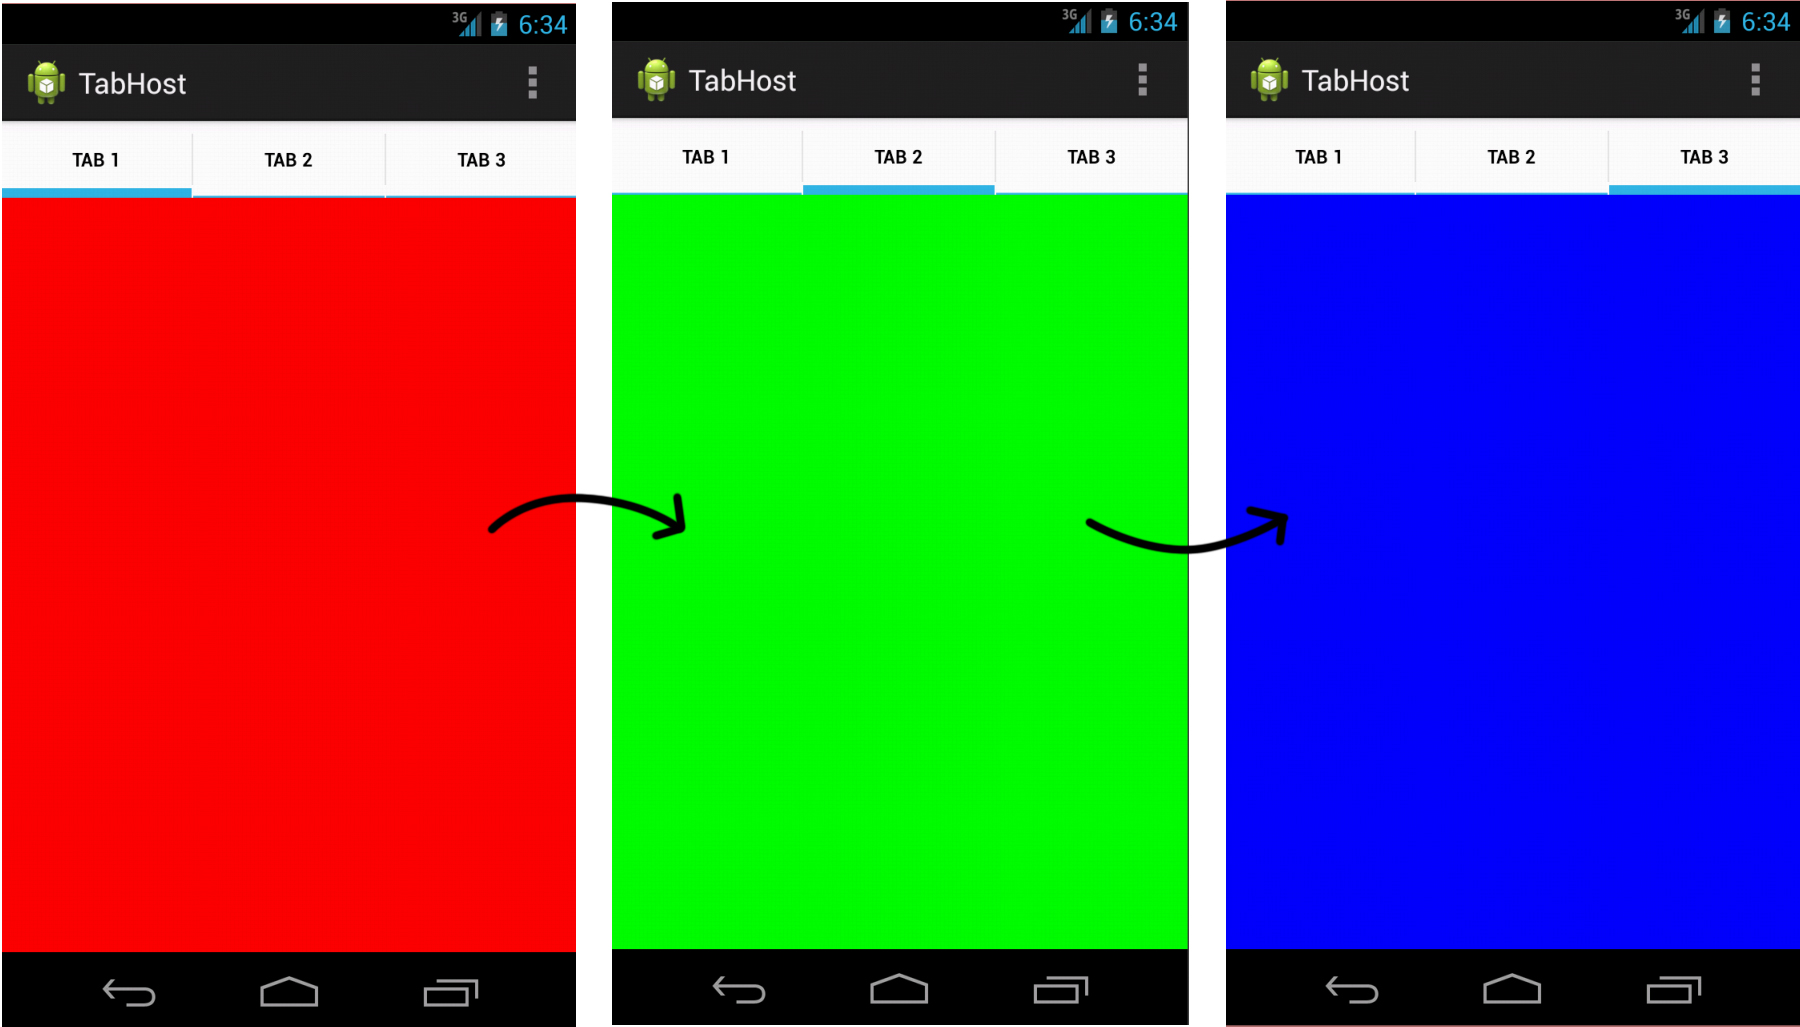
\includegraphics[width=1\textwidth]{figuras/design/tabs-rgb.jpg}
	  \caption{Figura mostrando as 3 abas criadas no exemplo}
	  \label{fig:e18}
	\end{figure}
	
	
% SWIPE %
\section{Trocar de página com gesto de arrastar usando \texttt{ViewPager}}

	É possível trocar entre fragmentos usando o gesto de arrastar, isto é, arrastando a tela de um lado para o outro acionará a troca entre os fragmentos. 
	
	Primeiro iremos definir o \emph{layout} do \texttt{ViewPager}\footnote{\href{http://developer.android.com/reference/android/support/v4/view/ViewPager.html}{http://developer.android.com/reference/android/support/v4/view/ViewPager.html}}. Depois iremos definir o \texttt{PagerAdapter}\footnote{\href{http://developer.android.com/reference/android/support/v4/view/PagerAdapter.html}{http://developer.android.com/reference/android/support/v4/view/PagerAdapter.html}}. Por último precisamos definir a \emph{activity} que irá conter o visualizador de páginas. 
	
	\begin{listing}[H]
	\inputminted[linenos=true,fontsize=\small,frame=lines, framesep=2mm, tabsize=2,numbersep=5pt]{xml}{src/design/viewpager.xml}
	\caption{\emph{layout} do \texttt{ViewPager}}
	\end{listing}
	
	Agora defina uma nova classe chamada \texttt{PagerAdapter} que irá estender a classe \\ \texttt{FragmentPagerAdapter}. Primeiro crie uma lista que irá conter os fragmentos, isto é, as páginas que serão exibidas. Ao estender essa classe precisamos implementar dois métodos: \texttt{getItem()} e \texttt{getCount()}. O método \texttt{getItem()}, na linha 10 do \hyperref[code:pageadap]{Algoritmo \ref*{code:pageadap}}, deve retornar o item que será selecionado pelo parâmetro \texttt{position}. O método \texttt{getCount()}, na linha 15, deve retornar a quantidade de páginas. Depois crie o construtor como mostrado nas linhas 4-7. 

	\begin{listing}[H]
	\inputminted[linenos=true,fontsize=\small,frame=lines, framesep=2mm, tabsize=2,numbersep=5pt]{java}{src/design/pageradapter.java}
	\caption{Classe \texttt{PagerAdapter}}
	\label{code:pageadap}
	\end{listing}
	
	Por último devemos construir a \emph{activity} que irá conter o \texttt{PagerAdapter} e será responsável por mostrar as páginas. Neste exemplo iremos reutilizar os fragmentos que fizemos na seção anterior quando trabalhamos com abas.
	
	\begin{framed}
	\paragraph{}\textbf{Dica}: Você pode importar as classes e os arquivos de \emph{layout}. No \emph{PackageExplorer} na IDE Eclipse, clique com o botão direito sobre a pasta que quer importar os arquivos, depois clique em \emph{Import} e selecione \emph{General -> File System}. Agora selecione o caminho da pasta que contém os arquivos no campo \emph{From directory}. Selecione os arquivos que deseja importar e clique em \emph{Finish}.
	Note que ao importar classes Java será necessário trocar o pacote a que a classe pertence.
	
	Outra opção é usar o \texttt{import} do java para importar as classes sem ter elas no pacote.
	
	\textit{}
	\end{framed}

	Essa \emph{activity}, como mostrada no \hyperref[code:act-pager]{Algoritmo \ref*{code:act-pager}} abaixo, apenas precisa instanciar os fragmentos (linhas 10,11 e 12), criar e determinar o adaptador, linhas 14, 16 e 17.
	
	\begin{listing}[H]
	\inputminted[linenos=true,fontsize=\small,frame=lines, framesep=2mm, tabsize=2,numbersep=5pt]{java}{src/design/viewpager-activity.java}
	\caption{\emph{Activity} com \texttt{PagerAdapter}}
	\label{code:act-pager}
	\end{listing}

% SWIPEABLE TABS %
\section{Abas com gesto de arrastar}

	Ao juntar os dois conceitos, o de \emph{layout} com abas e o gesto de arrastar, podemos fazer o controle das abas arrastando a tela. Esse tipo de \emph{design} é comum em muitos aplicativos pela facilidade e rapidez com o que o usuário pode visualizar vários conteúdos. 
	Nesse exemplo iremos reutilizar o código dos exemplos anteriores com algumas modificações. Serão reutilizadas classes: \texttt{TabInfo}, \texttt{TabFactory}, \texttt{PagerAdapter}, \texttt{Tab1Fragment}, \texttt{Tab2Fragment}, \texttt{Tab3Fragment}.
	
	Primeiro modificaremos o \emph{layout} das abas adicionando o \texttt{ViewPager} após \texttt{FrameLayout}. Note que esse é o mesmo \emph{layout} do \hyperref[code:layout-tabhost]{Algoritmo \ref*{code:layout-tabhost}}, por isso o \hyperref[code:layout-viewpager]{Algoritmo \ref*{code:layout-viewpager}} não está completo.
	
	\begin{listing}[H]
	\inputminted[linenos=true,fontsize=\small,frame=lines, framesep=2mm, tabsize=2,numbersep=5pt]{xml}{src/design/swipetabs-layout.xml}
	\caption{\emph{Layout} das abas com adição do \texttt{ViewPager}}
	\label{code:layout-viewpager}
	\end{listing}
	
	Agora iremos usar a classe \texttt{TabLayoutActivity} do exemplo anterior e fazer algumas alterações.  Nesse exemplo irei mudar o nome da classe para \texttt{SwipeTabActivity}. A primeira alteração é a adição de algumas variáveis para serem usadas na classe, adicione uma variável \texttt{PageAdapter} e uma \texttt{ViewPager}. Depois devemos alterar o método \texttt{onCreate()}, adicione uma chamada ao método \texttt{initialiseViewPager()}. A implementação é a mesma do método \texttt{onCreate()} do exemplo anterior com a adição da chamada ao método \\ \texttt{setOnPageChangeListener()}. Devemos também implementar a interface \\ \texttt{OnPageChangeListener}.\\ No método \texttt{initialiseTabHost()} você precisa remover a linha \texttt{onTabChanged(''Tab1'');}.
	
	\begin{listing}[H]
	\inputminted[linenos=true,fontsize=\small,frame=lines, framesep=2mm, tabsize=2,numbersep=5pt]{java}{src/design/initialiseviewpager.java}
	\caption{Método \texttt{initialiseViewPager()}}
	\end{listing}
	
	Em seguida precisamos alterar o método \texttt{onTabChanged()}, não necessitamos mais fazer verificações já que o próprio \emph{design} irá limitar as falhas que poderiam ocorrer. Precisamos apenas determinar para o \texttt{ViewPager} o item atual. 
	
	\begin{listing}[H]
	\inputminted[linenos=true,fontsize=\small,frame=lines, framesep=2mm, tabsize=2,numbersep=5pt]{java}{src/design/ontabchanged-swipe.java}
	\caption{Método \texttt{onTabChanged()} alterado}
	\end{listing}
	
	Por fim, devemos implementar os métodos da interface \\ \texttt{ViewPager.OnPageChangeListener}, somente o método \texttt{onPageSelected()} será usado, para selecionar a aba correspondente à pagina atual.
	
	\begin{listing}[H]
	\inputminted[linenos=true,fontsize=\small,frame=lines, framesep=2mm, tabsize=2,numbersep=5pt]{java}{src/design/vpinterface.java}
	\caption{Métodos da interface \texttt{ViewPager.OnPageChangeListener}}
	\end{listing}
		
	\begin{framed}
	\paragraph{}\textbf{Dica}: Pela dificuldade em acompanhar passo a passo a construção desse \emph{design}, é recomendável obter o código do projeto no repositório. Está sob o nome 		\emph{SwipeableTabs}.
	\textit{}
	\end{framed}
	
\section{\emph{ActionBar}}

	A \emph{ActionBar} é aquela barra presente em em todos os aplicativos que fizemos de exemplo até agora. Ela pode mostrar o nome da \emph{activity}, ícones, ações que podem ser acionadas, outras \emph{views} ou botões interativos. Também pode ser usada para navegar entre as \emph{actvities} do seu aplicativo.
	
	Dispositivos Android mais antigos possuem um botão físico chamado \emph{Option} que abre um menu na parte inferior do aplicativo. A \emph{ActionBar} é melhor que esse menu pois está claramente visível para o usuário, enquanto que o menu antigo era escondido e o usuário pode não reconhecer que as opções estão disponíveis.
	
	\begin{figure}[H]
	  \centering
	  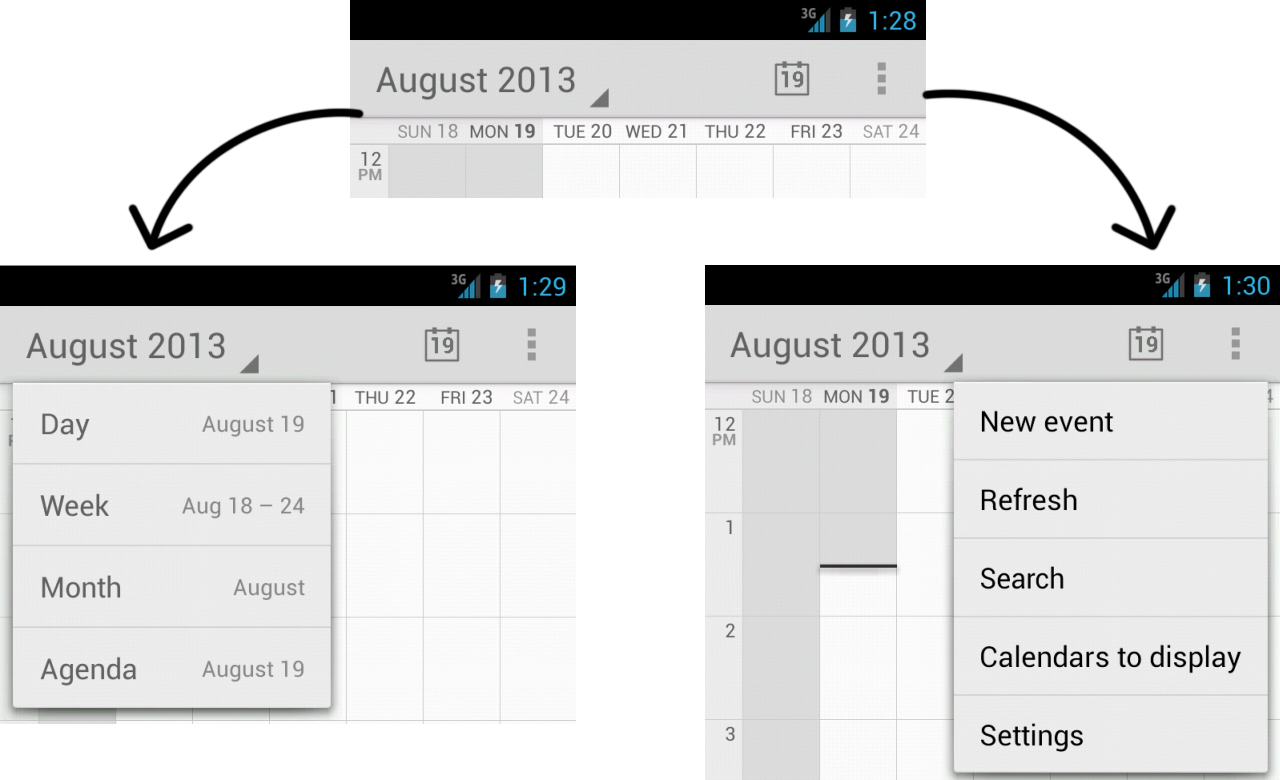
\includegraphics[width=.8\textwidth]{figuras/design/actionbar-ex.jpg}
	  \caption{Exemplo de \emph{ActionBar} no aplicativo Calendário}
	  \label{fig:e19}
	\end{figure}
	
	A \autoref{fig:e19} mostra o uso da \emph{ActionBar} no aplicativo Calendário, padrão dos aparelhos Android mais atuais. É possível observar três principais componentes. O primeiro é um menu \emph{drop-down} que permite ao usuário mudar o modo de visualização do calendário. O segundo é um botão com o dia atual, 19, que ao ser pressionado faz com que o calendário posicione um cursor no dia e hora atuais. O terceiro é um outro menu \emph{drop-down} com algumas opções que podem ser interessantes ao usuário.
	
	\subsection{Implementando a \emph{ActionBar}}
	
		A \emph{activity} popula a \emph{ActionBar} em seu método \texttt{onCreateOptionsMenu()}. Entradas na \emph{ActionBar} são chamadas de ações (\emph{actions}). 
		
		As ações para a \emph{ActionBar} são definidas em arquivos XML posicionados na pasta \texttt{menu/}. O \hyperref[code:actionbarNew]{Algoritmo \ref*{code:actionbarNew}} mostra o menu padrão dos exemplos que construímos até agora. Ele só contém um item \emph{''Settings''} que está no \emph{dropdown} menu que pode ser acessado através da \emph{ActionBar}, à direita. O fato dele estar escondido se deve ao atributo \texttt{showAsAction} estar com valor \emph{never}, ao ser mudado para \emph{always} o acesso ao \emph{Settings} será diretamente através da \emph{ActionBar}. Existe também o valor \emph{ifRoom} que irá mostrar apenas se houver espaço disponível.
		
		\begin{listing}[H]
		\inputminted[linenos=true,fontsize=\small,frame=lines, framesep=2mm, tabsize=2,numbersep=5pt]{xml}{src/design/actionbar-menupadrao.xml}
		\caption{Menu padrão dos exemplos}
		\end{listing}

		\begin{listing}[H]
		\inputminted[linenos=true,fontsize=\small,frame=lines, framesep=2mm, tabsize=2,numbersep=5pt]{java}{src/design/oncreateoptionsmenu-padrao.java}
		\caption{Método padrão \texttt{onCreateOptionsMenu()}}
		\label{code:actionbarNew}
		\end{listing}
		
		Se uma ação é selecionada, o método \texttt{onOptionsItemSelected()} é chamado. Ele recebe a ação selecionada como parâmetro \texttt{MenuItem}. Baseando-se nessa informação você pode decidir o que fazer. Nesse exemplo iremos abrir uma nova \emph{activity} que seria a tela de configuração do aplicativo.
		
		No seu projeto, crie uma nova \emph{Activity} do tipo \emph{Settings Activity}. 
		
		\begin{framed}
\paragraph{}\textbf{Dica}: Para criar uma nova \emph{activity}, clique com o botão direito sob o projeto selecione \emph{New -> Other} (ou pressione \emph{Ctrl+N}). Selecione \emph{Android Activity} e selecione o tipo desejado.
\textit{}
\end{framed}

		
		Agora você deve fazer com que o método \texttt{OnCreateOptionsMenu()} abra essa nova \emph{activity}.
		
		\begin{listing}[H]
		\inputminted[linenos=true,fontsize=\small,frame=lines, framesep=2mm, tabsize=2,numbersep=5pt]{java}{src/design/onoptionsitemselected.java}
		\caption{Método \texttt{OnOptionsItemSelected()}}
		\end{listing}

		Para melhorar nossa \emph{ActionBar} vamos adicionar um campo para pesquisa. Você pode adicionar \emph{views} em sua \emph{ActionBar}. Para isso você deve usar o método \texttt{setCustomView()}  da classe \texttt{ActionBar} e passar uma \emph{view} como parâmetro. Você também precisa ativar a exibição de \emph{views} com o método \texttt{setDisplayOptions()} e passar a \\ \emph{flag} \texttt{ActionBar.DISPLAY\_SHOW\_CUSTOM}.
		
		Primeiro vamos adicionar um ícone de busca na nossa \emph{ActionBar}, voltando ao arquivo do \emph{layout} da \emph{ActionBar}, adicione um novo item acima do primeiro como mostrado no \hyperref[code:actionbarNew2]{Algoritmo \ref*{code:actionbarNew2}}.
		
		\begin{listing}[H]
		\inputminted[linenos=true,fontsize=\small,frame=lines, framesep=2mm, tabsize=2,numbersep=5pt]{xml}{src/design/newitem.xml}
		\caption{Adicionando novo item na \emph{ActionBar}}
		\label{code:actionbarNew2}
		\end{listing}
		
		Observe o atributo \texttt{android:icon}, estamos obtendo um \emph{drawable} que já existe no sistema Android, e se chama \emph{ic\_menu\_search}. Esse é o ícone da busca, a lupa. Depois vamos adicionar uma ação a ser executada quando esse ícone for clicado. Iremos criar nesse exemplo, uma caixa de texto de forma programática, isto é, em vez de defini-la no XML iremos criá-la com código na \emph{Activity}. 
		
		No método \texttt{onCreate()} você precisa configurar a \emph{ActionBar} para mostrar \emph{views}. Use o método \texttt{getActionBar()} para obter uma referência da \emph{ActionBar} e \texttt{setDisplayOptions()} para configurá-la. Depois, no método \texttt{onOptionsItemSelected()} você vai programar a ação do novo botão. Inicialmente cria-se uma nova \emph{view} do tipo \texttt{EditText}, colocamos algumas configurações e a adicionamos na \emph{ActionBar}. Por não termos uma busca devidamente implementada, vamos mostrar um \texttt{Toast} com o conteúdo da busca, a fim de demonstração.
		
		\begin{listing}[H]
		\inputminted[linenos=true,fontsize=\small,frame=lines, framesep=2mm, tabsize=2,numbersep=5pt]{java}{src/design/actionbar-oncreate.java}
		\caption{Configurando \emph{ActionBar} no método \texttt{onCreate()}}
		\end{listing}
		
		No \hyperref[code:actionbar-seach]{Algoritmo \ref*{code:actionbar-seach}}, abaixo, criamos um \texttt{EditText} e o configuramos caso o botão com o ícone de busca seja pressionado. Na linha 5-6 criamos um \texttt{LayoutParams} que configura o tamanho da \emph{view}. Na linha 8 o método \texttt{EditText.setImeOptions()} é responsável por configurar o teclado para uma busca, junto com a linha 9 que diz para o \texttt{EditText} que a entrada será texto, essa combinação faz com que o teclado mostre o ícone da lupa no lugar da tecla \emph{Enter}. A linha 10 configura a cor do texto para branca. Adicionamos a \emph{view} na \emph{ActionBar} com o método \texttt{ActionBar.setCustomView()} e passamos como parâmetro a \emph{view} criada e os parâmetros de \emph{layout} criados. O método \texttt{EditText.requestFocus()} faz com que o foco seja dado à nova caixa de texto, para que possamos editá-la. Precisamos ainda fazer com que o teclado abra para que possamos editar a caixa de texto, é isso que as linhas 13-14 e 15 estão fazendo. O método \texttt{getSystemService()} obtém a referência de um serviço do Android, e nesse caso estamos pedindo pelo serviço de método de entrada, o teclado. O método \texttt{InputMethodManager.showSoftInput()} abre o \emph{Soft Input}, ou seja, o teclado virtual para edição da \emph{view}. 
		
		Finalmente fazemos com que ao botão de busca no teclado ser clicado, um \texttt{Toast} mostre para o usuário o conteúdo da caixa de texto. É isso que a interface \texttt{onEditorActionListener} faz com o método \texttt{onEditorAction()}.
		
		A intenção desse exemplo é mostrar como você pode adicionar novas \emph{views} na \emph{ActionBar} de forma dinâmica.
		 
		\begin{listing}[H]
		\inputminted[linenos=true,fontsize=\small,frame=lines, framesep=2mm, tabsize=2,numbersep=5pt]{java}{src/design/actionbar-acao.java}
		\caption{Criando a caixa de busca na \emph{ActionBar}}
		\label{code:actionbar-seach}
		\end{listing}
		
		
	\begin{figure}[H]
	  \centering
	  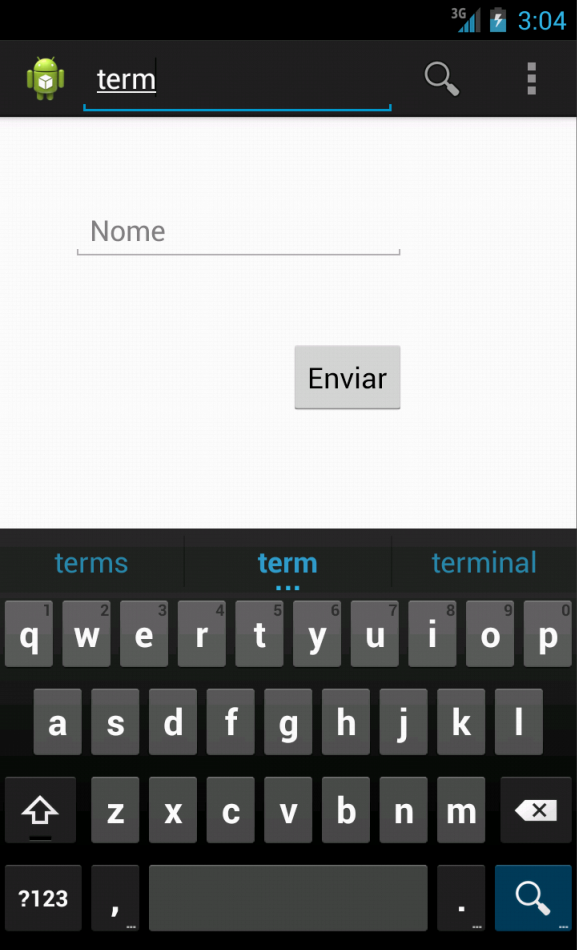
\includegraphics[width=.3\textwidth]{figuras/design/actionbar-search.png}
	  \caption{Exemplo de busca na \emph{ActionBar}}
	  \label{fig:e20}
	\end{figure}

%%%COMUNICAÇÃO%%%
\chapter{Comunicação}

	Agora iremos explorar as funcionalidades de comunicação dos aparelhos Android como acesso a \emph{Internet} no caso de \emph{Tables} e \emph{Smartphones} e envio de SMS e chamadas de voz com os os \emph{Smartphones}. 

\section{\emph{Internet}}

	Antes de iniciar sua aplicação que faz acesso à \emph{Internet}, devemos dar permissão ao aplicativo através do arquivo de \emph{Manifest}. Logo antes da tag \texttt{uses-sdk} você deve adicionar a tag \texttt{uses-permission}, como mostrado abaixo:

		\begin{listing}[H]
		\inputminted[linenos=true,fontsize=\small,frame=lines, framesep=2mm, tabsize=2,numbersep=5pt]{xml}{src/api/comm/permission-internet.xml}
		\caption{Atribuindo permissão de acesso à \emph{Internet} no \emph{Manifest}}
		\label{code:permission-internet}
		\end{listing}

		Nesta seção, veremos como se faz requisições HTTP para obter páginas HTML, saídas de um \emph{script server-side} como PHP ou ASP.NET e \emph{parsing} de respostas JSON ou XML.		 

		\subsection{HTTP GET}

		Para fazer uma requisição HTTP GET usaremos as classes da biblioteca \emph{Apache}, tais como \emph{HttpClient}, \emph{HttpGet} e \emph{HttpResponse}. Primeiros crie uma classe que iremos chamar de \texttt{RequestTask} e ela deve estender a classe \texttt{AsyncTask}\footnote{\href{http://developer.android.com/reference/android/os/AsyncTask.html}{http://developer.android.com/reference/android/os/AsyncTask.html}}, ela vai permitir que façamos a requisição na \emph{thread} da interface do usuário sem precisar criar e manipular uma \emph{thread} diferente.

		\begin{listing}[H]
		\inputminted[linenos=true,fontsize=\small,frame=lines, framesep=2mm, tabsize=2,numbersep=5pt]{java}{src/api/comm/asynctask.java}
		\caption{Classe \texttt{RequestTask}}
		\label{code:requesttask}
		\end{listing}

		O método \texttt{doInBackground()} é o responsável por realizar a operação sem o usuário perceber. Existem outros dois métodos da classe \texttt{AsyncTask} que podem ser utilizados: \texttt{onProgressUpdate()}, caso queira mostrar o progresso de um \emph{download} para o usuário e \texttt{onPostExecute()} para executar alguma ação após o termino do \emph{download}.

		Observe o \hyperref[code:requesttask]{Algoritmo \ref*{code:requesttask}}, na linha 5-7 criamos um novo \texttt{HttpClient}, \texttt{HttpResponse} e uma \emph{string} para armazenar a resposta do servidor. Depois, envolto por um bloco \texttt{try-catch} temos uma chamada ao método \texttt{HttpClient.execute()} e é passado para ele um novo \texttt{HttpGet} com o parâmetro \texttt{uri[0]}, \texttt{uri} é um dos parâmetros do método e contém uma URI\footnote{\href{http://developer.android.com/reference/java/net/URI.html}{http://developer.android.com/reference/java/net/URI.html}} que identifica o destino da requisição.

		Na linha 11 foi criado um novo \texttt{StatusLine}\footnote{\href{http://developer.android.com/reference/org/apache/http/StatusLine.html}{http://developer.android.com/reference/org/apache/http/StatusLine.html}} para guardar a resposta da requisição HTTP que obtemos com o método \texttt{HttpResponse.getStatusLine()}. Depois comparamos o código do \emph{status} com \texttt{HttpStatus.SC\_OK} (equivalente ao código 200), o \emph{status} \texttt{OK} significa que a requisição e a resposta ocorreram como esperado e temos a resposta correta vindo do servidor. 

		Em seguida criamos um novo \texttt{ByteArrayOutputStream} que é responsável por guardar a resposta do servidor na chamada ao método \texttt{HttpResponse.getEntity().writeTo()}. Por último convertemos o \emph{byte stream} em uma string usando o método \texttt{toString()} e a retornamos.

		Agora precisamos de uma \emph{Activity} para mostrar a resposta, nesse exemplo obteremos o código HTML da página do DC UFSCar: \href{http://www.dc.ufscar.br}{http://www.dc.ufscar.br}. Mostraremos o código HTML como uma página \emph{Web} usando o \texttt{WebView}.

		\begin{listing}[H]
		\inputminted[linenos=true,fontsize=\small,frame=lines, framesep=2mm, tabsize=2,numbersep=5pt]{java}{src/api/comm/httpget.java}
		\caption{Usando \texttt{RequestTask} na \emph{activity}}
		\label{code:requestactivity}
		\end{listing}		

		Primeiro criamos uma nova variável \texttt{task} do tipo \texttt{AsyncTask} nos moldes da classe que criamos, dentro de um bloco \texttt{try-catch} criamos uma nova \texttt{URI} e atribuímos a ela o endereço da página do DC UFSCar. Em seguida iniciamos a variável \texttt{task} criando uma nova \texttt{RequestTask} e chamamos o método \texttt{execute()}, que ao ser chamado irá executar o método \texttt{doInBackground()}. 
		
		Por fim, criamos uma nova \texttt{WebView}\footnote{\href{http://developer.android.com/reference/android/webkit/WebView.html}{http://developer.android.com/reference/android/webkit/WebView.html}} e carregamos o conteúdo da \emph{string} \texttt{response} nela usando o método \texttt{WebView.loadData()}. A página é mostrada sem estilo pois não estamos puxando as folhas de estilo junto, somente o código HTML.
		 
		 \begin{framed}
\paragraph{}\textbf{Dica}: Usamos a \texttt{WebView} para mostrar o código HTML como página apenas para demonstração. Caso queira carregar uma página corretamente deve fornecer a \emph{URL} da página diretamente para a \texttt{WebView}.
\textit{}
\end{framed}

		\subsection{HTTP POST}
		Diferentemente do \emph{GET}, onde os parâmetros para o servidor vão codificados na \emph{URL}, no \emph{POST} os parâmetros vão codificados no final do cabeçalho HTTP. Para enviar uma requisição do tipo \emph{POST}, usaremos a classe \texttt{HttpPost}. O algoritmo abaixo é reaproveitado da classe \texttt{RequestTask} e do método \texttt{doInBackgrond()}, onde mudaremos apenas algumas linhas. Agora estaremos enviando a requisição para essa página: \href{http://httpbin.org/post}{http://httpbin.org/post}, ela só aceita requisições do tipo \emph{POST}, se tentar com \emph{GET} irá receber uma mensagem de erro.

		\begin{listing}[H]
		\inputminted[linenos=true,fontsize=\small,frame=lines, framesep=2mm, tabsize=2,numbersep=5pt]{java}{src/api/comm/httppost.java}
		\caption{Modificando o método para requisições \emph{POST}}
		\label{code:httppost}
		\end{listing} 

		Criamos um novo \texttt{HttpPost}\footnote{\href{http://developer.android.com/reference/org/apache/http/client/methods/HttpPost.html}{http://developer.android.com/reference/org/apache/http/client/methods/HttpPost.html}} passando a \texttt{URI} como parâmetro. Criamos uma lista de tuplas chave-valor que representa a variável e seu valor no cabeçalho HTTP e adicionamos dois valores. Em seguida chamamos o método \texttt{HttpPost.setEntity()} e passamos um objeto do tipo \texttt{UrlEncodedFormEntity}\footnote{\href{http://developer.android.com/reference/org/apache/http/client/entity/UrlEncodedFormEntity.html}{http://developer.android.com/reference/org/apache/http/client/entity/UrlEncodedFormEntity.html}} que recebe a lista como parâmetro, esse objeto irá codificar a lista em variáveis aceitas pelo padrão de uma requisição \emph{POST}.

		Por final, executamos a requisição como feito anteriormente. O resto do código é igual.

 		Note que se colocar a resposta dessa requisição em uma \texttt{WebView} ou \texttt{TextView} irá observar que está codificado no formato JSON\footnote{O que é JSON: \href{http://www.json.org/}{http://www.json.org/}}. 

		\subsection{Decodificando JSON}
		
		Vamos obter dados do objeto JSON retornado pelo exemplo anterior. Se você observar a \emph{string} na tela, irá perceber os dados que foram enviado via \emph{POST} dentro de um objeto JSON chamado \emph{form}. Queremos obter esses dados, para isso precisamos criar uma classe que será responsável por obter especificamente esses dados do \emph{form}.
		
\begin{framed}
\paragraph{}\textbf{Dica}: Em JSON, \{ representa um objeto JSON e [ representa um \emph{array} dentro de um objeto JSON
\textit{}
\end{framed}

		Crie uma classe \texttt{JSONParser}, como mostrado abaixo.
		
		\begin{listing}[H]
		\inputminted[linenos=true,fontsize=\small,frame=lines, framesep=2mm, tabsize=2,numbersep=5pt]{java}{src/api/comm/jsonparser.java}
		\caption{Classe \texttt{JSONParser}}
		\label{code:jsonparser}
		\end{listing} 

		Para obter dados do \emph{form}, criamos um método \texttt{getFormData()}. Primeiro obtemos o objeto JSON dado pela \emph{string} retornada pela requisição \emph{POST} do exemplo anterior ao criar um novo \texttt{JSONObject} e passando a \emph{string} como parâmetro. Em seguida queremos obter outro objeto JSON, aquele cujo nome é \emph{form}, para isso chamamos o método \\ \texttt{JSONObject.getJSONObject()} passando o nome do objeto junto. Após obter o objeto desejado, usamos o método \\ \texttt{JSONObject.getString()} e passamos o nome do valor para obter o valor. Então ao passar \emph{"testing"} e \emph{"user"} esperamos como retorno \emph{POST} e \emph{You}, respectivamente. 

		\subsection{Codificando JSON}

		Podemos também codificar objetos JSON, e é simples. Basta criar um \texttt{JSONObject} ou \texttt{JSONArray} e usar o método \texttt{toString()}. Por exemplo:
	
		\begin{listing}[H]
		\inputminted[linenos=true,fontsize=\small,frame=lines, framesep=2mm, tabsize=2,numbersep=5pt]{java}{src/api/comm/writejson.java}
		\caption{Criando JSON}
		\label{code:jsonparser2}
		\end{listing} 


	\section{Telefone}
		
		É possível fazer uma chamada telefônica, porém você terá que usar o discador padrão do Android uma vez que ele não provê uma API pública para fazer chamadas diretamente pelo seu aplicativo. A única forma é através do intermediador \texttt{ACTION\_CALL}. O Exemplo abaixo mostra como fazer uma chamada usando esse intermediador.

		\begin{listing}[H]
		\inputminted[linenos=true,fontsize=\small,frame=lines, framesep=2mm, tabsize=2,numbersep=5pt]{java}{src/api/comm/phonecall.java}
		\caption{Fazendo uma chamada telefônica}
		\label{code:phonecall}
		\end{listing} 

		Para esse exemplo, foi criado uma caixa de texto e um botão, o número de telefone é colocado na caixa de texto e o botão \emph{Call} inicia a \emph{activity} responsável por realizar a chamada. Observe que é necessário fazer um \emph{parse} do número de telefone para uma \emph{URI} com formato \texttt{tel:0123456789}. Cria-se uma \texttt{Intent} para o \texttt{ACTION\_CALL}, coloca-se os dados na \texttt{Intent} e chama o método \texttt{startActivity()} para fazer a chamada telefônica. É preciso dar permissão ao aplicativo para fazer chamadas adicionando essa linha ao \emph{Manifest}.
	
		\begin{listing}[H]
		\inputminted[linenos=true,fontsize=\small,frame=lines, framesep=2mm, tabsize=2,numbersep=5pt]{xml}{src/api/comm/phonecall-perm.xml}
		\caption{Permissão para fazer chamadas telefônicas}
		\label{code:phonecall-perm}
		\end{listing} 		

		Usando a classe \texttt{TelephonyManager}\footnote{\href{http://developer.android.com/reference/android/telephony/TelephonyManager.html}{http://developer.android.com/reference/android/telephony/TelephonyManager.html}}, no entanto, o Android nos dá a possibilidade obter dados do \emph{Sim Card} e também um \emph{listener} para saber o status atual do telefone, se ele está fazendo uma ligação ou não.

		Você pode usar os métodos \texttt{getDeviceId()} para obter o número IMEI do aparelho, \texttt{getSimSerialNumber()} para obter o número de série do \emph{Sim Card}, \texttt{isNetworkRoaming()} para saber se está em modo \emph{roaming}, etc.

	\section{\emph{Short Message Service (SMS)}}

		O Android provê uma API pública para mandar mensagens SMS, através da classe \texttt{SMSManager}\footnote{\href{http://developer.android.com/reference/android/telephony/SmsManager.html}{http://developer.android.com/reference/android/telephony/SmsManager.html}}. Assim como fazer ligações, enviar SMS também precisa configurar a permissão no \emph{Manifest}.

		\begin{listing}[H]
		\inputminted[linenos=true,fontsize=\small,frame=lines, framesep=2mm, tabsize=2,numbersep=5pt]{xml}{src/api/comm/sms-perm.xml}
		\caption{Permissão para enviar mensagens SMS}
		\label{code:sms-perm}
		\end{listing} 	

		Agora vamos criar um aplicativo simples que chama a classe \texttt{SMSManager} para enviar uma mensagem para um número de telefone. Teremos duas \texttt{EditText} \emph{views} para abrigar a mensagem e o número, e um botão para enviar. Inicialmente crie um método \texttt{sendSMS()}.

		\begin{listing}[H]
		\inputminted[linenos=true,fontsize=\small,frame=lines, framesep=2mm, tabsize=2,numbersep=5pt]{java}{src/api/comm/sendsms.java}
		\caption{Método \texttt{sendSMS()}}
		\label{code:sendsms}
		\end{listing} 	
	
		Dentro de um bloco \texttt{try-catch} crie um novo \texttt{SMSManager} como mostrado na linha 3 do  \hyperref[code:sendsms]{Algoritmo \ref*{code:sendsms}}, use o método \texttt{SmsManager.sendTextMessage()} para enviar uma mensagem. O primeiro parâmetro é o número de telefone para qual a mensagem será enviada, o segundo é o telefone de origem, colocando \texttt{null} o valor será o número do próprio aparelho ou serviço, o terceiro parâmetro é o texto da mensagem.
		
		Completando, com um algoritmo simples para chamar o método quando o botão for pressionado.

		\begin{listing}[H]
		\inputminted[linenos=true,fontsize=\small,frame=lines, framesep=2mm, tabsize=2,numbersep=5pt]{java}{src/api/comm/sendsms-oncreate.java}
		\caption{Chamando método \texttt{sendSMS()}}
		\label{code:sendsms2}
		\end{listing} 	

%%%ARMAZENAMENTO%%%
\chapter{Armazenamento}

	O Android provê algumas opções para que você possa salvar dados persistentes de sua aplicação. A escolha da opção de armazenamento vai depender das necessidades da sua aplicação, isto é, se os dados vão ser visíveis somente pela aplicação ou se o usuário terá acesso a eles, quanto de espaço será necessário, que tipo de dados você pretende salvar.
	As opções são: 
	\bi
		\item \emph{Shared Preferences}: Usada principalmente para salvar preferências do usuário, esse método guarda primitivas em duplas chave-valor;
		\item Armazenamento Interno: Salva dados privados na memória do dispositivo;
		\item Armazenamento externo: Salva dados públicos na memória externa compartilhada;
		\item Banco de Dados \emph{SQLite}: Salva dados estruturados em um banco de dados privado.
		\item Conexão com a rede: Salva dados na \emph{web} em seu próprio servidor na rede.
	\ei
			
	\section{\emph{Shared Preferences:}}
		
		A classe \texttt{SharedPreferences}\footnote{\href{http://developer.android.com/reference/android/content/SharedPreferences.html}{http://developer.android.com/reference/android/content/SharedPreferences.html}} fornece um framework que te permite salvar e recuperar dados primitivos persistentes no formato chave-valor. Você pode salvar qualquer tipo de dado primitivo: \emph{booleans}, \emph{floats}, inteiros, \emph{longs} e \emph{strings}.
 
		Você pode usar essa classe para armazenar dados durante o ciclo de vida de uma \emph{activity}. Isto é, antes da \emph{activity} ser destruída na função \texttt{onDestroy()}, os dados podem ser salvos durante a execução de \texttt{onStop()} e recuperados na execução de \texttt{onCreate()}.

		Para usar a \texttt{SharedPreferences} na sua aplicação você deve chamar \\ \texttt{getSharedPreferences()} se precisar de vários arquivos de preferencias que serão identificados pelo nome ou \\ \texttt{getPreferences()} se precisar de apenas um arquivo para sua \emph{activity}, esse não necessita de nome pois será único para a \emph{activity}. Em seguida para escrever valores você deve chamar o método \texttt{edit()} para obter um \texttt{SharedPreferences.Editor}, e usar os métodos como \texttt{putString()} para adicionar novos valores. Por último \texttt{commit()} deve ser chamado para salvar os valores. Para ler os valores, você deve chamar métodos como \texttt{getBoolean()} ou \texttt{getString()}.

		O exemplo abaixo salva os dados de uma caixa de texto, uma barra de progresso e uma chave em uma \texttt{SharedPreferences} e depois os lê quando o aplicativo é aberto novamente.

		\begin{listing}[H]
		\inputminted[linenos=true,fontsize=\small,frame=lines, framesep=2mm, tabsize=2,numbersep=5pt]{java}{src/api/storage/sharedpref.java}
		\caption{Utilizando \texttt{SharedPreferences} para salvar dados primitivos}
		\label{code:sharedpref}
		\end{listing} 	
		
		Observe no algoritmo \hyperref[code:sharedpref]{Algoritmo \ref*{code:sharedpref}} a utilização da classe \texttt{SharedPreferences}, no método \texttt{onStop()} chamamos o método \texttt{getPreferences(MODE\_PRIVATE)} para obter uma instância da classe no modo privado, isto é, os dados somente são acessíveis por esta \emph{activity} deste aplicativo. Na linha 30 obtemos o \texttt{SharedPreferences.Editor} ao chamar o método \texttt{SharedPreferences.edit()}.
		
		O \texttt{Editor} é usado então para adicionar os valores que obtemos das \emph{views}. Na linha 32 usamos \texttt{putString()} para guardar o conteúdo da caixa de texto,
\texttt{putInt()} para guardar a posição da \texttt{SeekBar} e \texttt{putBoolean()} para guardar o estado da chave. Finalmente invocamos \texttt{commit()} para salvar os dados.

		No método \texttt{onCreate()} usamos os métodos \texttt{get} para obter os dados que foram salvos. Esses métodos requerem a passagem de um valor \emph{default} para quando não há dados previamente salvos. Observe então nas linhas 16-18 que para a caixa de texto usamos uma \emph{string} vazia, para a \texttt{SeekBar} o valor 0 e a chave desligada.


		\section{Armazenamento interno}

		Você pode salvar arquivos diretamente na memória interna do dispositivo. Por padrão os arquivos salvos no armazenamento interno são privados a seu aplicativo e não podem ser acessados por outros aplicativos. 

		Para criar um novo arquivo você deve invocar o método \texttt{openFileOutput()} passando o nome do arquivo e o modo de operação. Esse método irá retornar um \texttt{FileOutputStream}. Você poderá escrever nesse arquivo chamando o método \texttt{FileOutputStream.write()} e \texttt{FileOutputStream.close()} para fechar o arquivo.

		Para exemplificar, faremos um aplicativo do tipo bloco de notas. Será composto de dois botões, um para abrir um arquivo e outro para salvar um arquivo, e uma caixa de texto para escrever. Tudo será feito no método \texttt{onCreate()}, primeiro  usamos \texttt{findViewById()} para obter as \emph{views}. O botão de salvar irá abrir um alerta perguntando o nome do arquivo, e o botão de abrir mostrará um alerta permitindo ao usuário escolher dentre os arquivos já salvos anteriormente.

		No código abaixo criamos o \emph{listener} do botão de salvar, dentro dele criamos um alerta e precisamos de um \emph{listener} para confirmar e um para cancelar.

		\begin{listing}[H]
		\inputminted[linenos=true,fontsize=\small,frame=lines, framesep=2mm, tabsize=2,numbersep=5pt]{java}{src/api/storage/internal1.java}
		\caption{Passos iniciais do \emph{listener}, criando um alerta.}
		\label{code:internal1}
		\end{listing} 	
		\newpage
		Com o \texttt{AlertDialog.Builder} começamos a construir um novo alerta. Usamos o \texttt{LayoutInflater} para carregar o \emph{layout} com uma \texttt{EditText}.
		\\ Chamamos \texttt{setPositivoButton()} para criar um \emph{listener} que irá salvar o arquivo quando o botão for clicado.

		\begin{listing}[H]
		\inputminted[linenos=true,fontsize=\small,frame=lines, framesep=2mm, tabsize=2,numbersep=5pt]{java}{src/api/storage/internal2.java}
		\caption{Salvando um arquivo e mostrando um \texttt{Toast}}
		\label{code:internal2}
		\end{listing} 	

		Vamos analisar o \hyperref[code:internal2]{Algoritmo \ref*{code:internal2}}. Na linha 5 queremos a referência ao \texttt{EditText} contido no alerta, para isso precisamos usar a variável \texttt{fnameEntry} criada ao chamar o método \texttt{LayoutInflater.inflate()}. Depois, na linha 7-8 certificamos que o nome do arquivo não será vazio (se for vazio, o arquivo não é salvo), para isso atribuímos o nome \emph{untitled} a ele. Obtemos também o texto escrito na caixa de texto da \emph{activity} na linha 9.

		Agora que já temos o nome e os dados do arquivo, precisamos efetivamente salvá-lo no armazenamento interno. Com o método \texttt{openFileOutput()} teremos um \texttt{FileOutputStream} que servirá para escrever os dados no arquivo. Isso é feito nas linhas 13-14 com o método \texttt{write()} e em seguida o método \texttt{close()}.
		Para certificar ao usuário que o arquivo foi salvo, mostramos um \texttt{Toast} com a mensagem que o arquivo foi salvo.

		Se o usuário clicar em \emph{cancel} no alerta, precisamos fechá-lo, basta invocar \texttt{dialog.close()} no \emph{listener}.

		\begin{listing}[H]
		\inputminted[linenos=true,fontsize=\small,frame=lines, framesep=2mm, tabsize=2,numbersep=5pt]{java}{src/api/storage/internal3.java}
		\caption{Fechando o alerta ao clicar em \emph{close}}
		\label{code:internal3}
		\end{listing} 	

		Depois chame \texttt{builder.create().show()} no \texttt{listener} do botão \emph{Save} para mostrar o alerta.
 
		Para o botão \emph{Open} iremos mostrar um alerta com os nomes dos arquivos salvos anteriormente, quando um desses for clicado o arquivo se abrirá preenchendo a caixa de texto.

		\begin{listing}[H]
		\inputminted[linenos=true,fontsize=\small,frame=lines, framesep=2mm, tabsize=2,numbersep=5pt]{java}{src/api/storage/internal4.java}
		\caption{Criando um alerta com os arquivos salvos}
		\label{code:internal4}
		\end{listing} 	
	
		Dessa vez usamos o método \texttt{builder.setItems()} para construir uma lista no alerta. O método \texttt{fileList()} retorna um \texttt{array} de nomes de arquivo que foram armazenados internalmente no aplicativo. 

		\begin{listing}[H]
		\inputminted[linenos=true,fontsize=\small,frame=lines, framesep=2mm, tabsize=2,numbersep=5pt]{java}{src/api/storage/internal5.java}
		\caption{Criando um alerta com os arquivos salvos}
		\label{code:internal5}
		\end{listing} 	
		
		Na linha 7 do \hyperref[code:internal5]{Algoritmo \ref*{code:internal5}} queremos obter a referência do arquivo selecionado. Chamando o método \texttt{getFilesDir()} nos é fornecido o diretório contendo os arquivos, com \texttt{listFiles()} temos um \emph{array} de \texttt{Files} e o selecionamos com a variável \texttt{which}, que é a posição clicada na lista do alerta. Para ler os dados desse arquivo, usamos a classe \texttt{BufferedReader} e guardamos as linhas sendo lidas em um objeto do tipo \texttt{StringBuilder}. Nas linhas 13-16 lemos cada linha do arquivo em um loop \emph{while} e usamos o método \texttt{append()} duas vezes, uma para adicionar a linha lida na \emph{string} e outra para adicionar o separador de linha (comumente \textbackslash n). Ao fim invocamos \texttt{close()} para fechar o \texttt{BufferedReader}. E colocamos o texto lido de volta na caixa de texto.

\begin{framed}
\paragraph{}\textbf{Dica}: Você também pode optar por salvar seus arquivos no \emph{cache}, isto é, na pasta \emph{cache} da sua aplicação. Esses arquivos são apagados automaticamente quando o sistema necessita de memória. Para isso use o método \texttt{getCacheDir()} para obter o caminho do diretório de \emph{cache}.
\textit{}
\end{framed}

		\section{Armazenamento externo}

		Todo dispositivo Android suporta um armazenamento externo que é compartilhado e que pode ser usado para salvar arquivos. Esse armazenamento pode ser tanto um cartão SD que esta conectado ao aparelho como a própria memória interna dele. Os arquivos salvos no armazenamento externo podem ser lidos por todos outros aplicativos e modificados quando o usuário conecta ao computador para transferir os arquivos via USB.

		Se um dispositivo usa uma partição da memória interna do aparelho como armazenamento externo e ainda oferecer um cartão SD, então a partição do cartão SD não estará disponível para armazenamento, sua aplicação não conseguirá acessar o cartão SD. 

		Por isso, o armazenamento externo pode ficar indisponível caso o usuário monte o armazenamento externo no computador ou remova o cartão SD. Os arquivos são abertos e podem ser abertos, modificados ou removidos pelo usuário ou por outras aplicações.

		Para poder usar o armazenamento externo, primeiro você deve verificar sua disponibilidade usando o método \texttt{getExternalStorageState()}. A mídia pode estar conectada a um computador, faltando ou em estado de apenas leitura. Você pode verificar a disponibilidade da mídia como mostrado no exemplo abaixo, retirado da documentação oficial\footnote{\href{http://developer.android.com/guide/topics/data/data-storage.html\#filesExternal}{http://developer.android.com/guide/topics/data/data-storage.html\#filesExternal}}.

		\begin{listing}[H]
		\inputminted[linenos=true,fontsize=\small,frame=lines, framesep=2mm, tabsize=2,numbersep=5pt]{java}{src/api/storage/external1.java}
		\caption{Verificando se o armazenamento externo está disponível}
		\label{code:external1}
		\end{listing} 	

		O \hyperref[code:external1]{Algoritmo \ref*{code:external1}} verifica se o armazenamento externo está disponível. Temos duas variáveis de controle que guardarão o estado da mídia,\texttt{mExternalStorageAvailable} e \texttt{mExternalStorageWriteable}. A primeira nos diz se o armazenamento externo está disponível e a segunda se é possível escrever nele. Na variável \texttt{state} é guardado o estado que é obtido através do método \texttt{getExternalStorageState()}. Uma comparação é feita com o resultado obtido, se for equivalente à \texttt{Environment.MEDIA\_MOUNTED} então sabemos que a mídia está montada e é possível escrever nela, então setamos os estados das variáveis de controle para \texttt{true}. Caso o resultado seja equivalente à \texttt{Environment.MEDIA\_MOUNTED\_READ\_ONLY} então sabemos que a mídia está montada porém está somente com permissão de leitura, nesse caso setamos apenas a variável de disponibilidade como \texttt{true} e mantemos a outra como \texttt{false}. Se o resultado não for esses dois estados, mas sim algum outro estado possível, então setamos as duas variáveis para \texttt{false}.

		Após verificar a disponibilidade, você deve usar o método \texttt{getExternalFilesDir()} para obter uma referência ao caminho do diretório onde você deve salvar seus arquivos. Esse método recebe um parâmetro que especifica o tipo de subdiretório que você quer usar, tais como \texttt{DIRECTORY\_MUSIC} e \texttt{DIRECTORY\_RINGTONES}, ou passe \texttt{null} para obter a raiz dos diretórios da sua aplicação. O método irá criar o diretório apropriado se necessário. Ao especificar o tipo, você se assegura que o Android irá categorizar seus arquivos de forma apropriada. Se o usuário desinstalar seu aplicativo, todos os dados serão apagados.

		Se você quer salvar arquivos que não são específicos da sua aplicação e que não devem ser apagados quando desinstalado, salve-os em um dos diretórios públicos que estão no raiz da mídia de armazenamento externo. São eles os diretórios \texttt{Music/}, \texttt{Pictures/}, etc. Use o método \texttt{getExternalStoragePublicDirectory()} passando o tipo de diretório desejado, da mesma forma que anteriormente.

		O sistema classifica os arquivos encontrados nessas pastas na forma:

		\begin{itemize}
			\item \texttt{Music/} - Músicas do usuário;
			\item \texttt{Podcasts/} - \emph{podcasts};
			\item \texttt{Ringtones/} - Toques;
			\item \texttt{Alarms/} - Toques do despertador;
			\item \texttt{Notifications/} - Toques das notificações;
			\item \texttt{Pictures/} - Fotos (exceto aquelas tiradas com a câmera);
			\item \texttt{Movies/} - Filmes (exceto aquelas gravadas com a câmera); e
			\item \texttt{Download/} - Arquivos baixados.
		\end{itemize}

		\section{Banco de dados}

		O Android fornece suporte ao bancos de dados \texttt{SQLite}. Qualquer banco que você criar será acessível apenas pela sua aplicação e não fora dela.

		A maneira recomendada de criar um banco de dados é criando uma subclasse da classe \texttt{SQLiteOpenHelper} e sobrescrever o método \texttt{onCreate()}. Para ler e escrever no banco, chame os métodos \texttt{getReadableDatabase()} e \texttt{getWritableDatabase()}. Ambas retornam um objeto do tipo \texttt{SQLiteDatabase} que fornece métodos para operar sobre o banco.

		Usando o método \texttt{SQLiteDatabase.query()}  podemos realizar uma consulta, o método aceita vários parâmetros, tais como: tabela, seleção, colunas, agrupamento e etc. Para consultas mais complexas você pode usar a classe \texttt{SQLiteQueryBuilder} que contém vários métodos para construir consultas.

		Toda consulta vai retornar um \texttt{Cursor} que aponta para as tuplas do resultado da consulta. Você deverá usá-lo para navegar através dos resultados.

		Para exemplificar, vamos fazer um mecanismo simples de busca. O banco será populado com fabricantes de carros e alguns de seus modelos. Para o \emph{design} desse exemplo, optei por ter dois \emph{Spinners} (equivalente ao \emph{Combo Box}) e um botão. Os \emph{Spinners} serão populados com os dados do Banco de Dados de forma que o primeiro contenha todos os fabricantes de carros e o segundo todos os anos de fabricação de seus modelos, esses dados serão obtidos através de consultas ao banco.

		Para começar, devemos  criar o BD e isso é feito com uma classe que iremos criar que irá ser subclasse de \texttt{SQLiteOpenHelper}
\footnote{\href{http://developer.android.com/reference/android/database/sqlite/SQLiteOpenHelper.html}{http://developer.android.com/reference/android/database/sqlite/SQLiteOpenHelper.html}}.
 Chamaremos de \texttt{CarOpenHelper}. Essa classe tem algumas funções básicas, como criar e popular o BD, configurar a ação a ser tomada quando o BD é atualizado ou desatualizado.

		O \hyperref[code:db1]{Algoritmo \ref*{code:db1}} demonstra a criação do BD usado no exemplo:

		\begin{listing}[H]
		\inputminted[linenos=true,fontsize=\small,frame=lines, framesep=2mm, tabsize=2,numbersep=5pt]{java}{src/api/storage/db1.java}
		\caption{Classe \texttt{CarOpenHelper} do SQLite}
		\label{code:db1}
		\end{listing} 	

		Primeiro criamos algumas \emph{Strings} para ajudar na criação do banco. Em seguida, criamos o construtor da classe, os argumentos passados são: o contexto da \emph{activity} que instanciou a classe, o nome do banco, um \texttt{CursorFactory} caso esteja usando (não é o caso), e a versão do banco que começa em 1 e deve incrementar a medida que você o atualiza. 
		
		O método \texttt{onCreate()} do banco é responsável pela criação do banco e de o popular. Fazemos isso executando consultas SQL diretamente ao banco com o método \texttt{execSQL()}. No \hyperref[code:db1]{Algoritmo \ref*{code:db1}} você pode observar a chamada de \texttt{execSQL()} duas vezes. Não se confunda com a segunda consulta, que adiciona as tuplas ao banco, é só uma maneira de inserir várias tuplas em uma única consulta.

		Agora na nossa \emph{activity} precisamos realizar as consultas para popular os \emph{Spinners}. No método \texttt{onCreate()} faça: 

		\begin{listing}[H]
		\inputminted[linenos=true,fontsize=\small,frame=lines, framesep=2mm, tabsize=2,numbersep=5pt]{java}{src/api/storage/db2.java}
		\caption{Usando o \texttt{CarOpenHelper} na \emph{activity}}
		\label{code:db2}
		\end{listing} 	

		Estou "pulando" a parte de obter as referências dos \emph{spinners} e botões e partindo para o que interessa no código \hyperref[code:db2]{Algoritmo \ref*{code:db2}}. Na linha 5 instanciamos o \texttt{CarOpenHelper} na variável \texttt{mDatabase}. Na linha 6 criamos um \emph{array} que contém as colunas que iremos fazer consulta, isto é necessário para o método \texttt{query()} na linha 10.

		Ao chamar \texttt{mDatabase.getReadableDatabase()} obtemos um objeto do tipo \\ \texttt{SQLiteDatabase}
\footnote{\href{http://developer.android.com/reference/android/database/sqlite/SQLiteDatabase.html}{http://developer.android.com/reference/android/database/sqlite/SQLiteDatabase.html}}
 mas que só permite a leitura. Já o método \texttt{query()} retorna um \texttt{Cursor} que é usado para iterar sobre os resultados. Na linha 10 observe os parâmetros que usamos para fazer a consulta: A tabela que vamos fazer a consulta, um \emph{array} de \emph{strings} com as colunas que queremos obter,  uma cláusula \texttt{WHERE} (observe que passar \textbf{null} aqui implica em retornar todas as tuplas da coluna), argumentos da seleção (para aqueles que conhecem \emph{prepared statements} onde "?" é substituído pelos valores, uma cláusula \texttt{GROUP BY} (\textbf{null} significa não agrupar), uma cláusula \texttt{HAVING}, uma cláusula \texttt{ORDER BY} e uma cláusula \texttt{LIMIT}.

	Em seguida criamos dois \texttt{Set} para armazenar os resultados e omitir os repetidos. Usamos o \texttt{Cursor} para iterar sobre o resultado e adicioná-los aos conjuntos. O \texttt{set1} contém os fabricantes e o \texttt{set2} contém os anos de fabricação. Usamos \texttt{Cursor.getString()} para obter o elemento do resultado que está naquele índice, nesse caso o índice 0 é a coluna de fabricantes e o índice 1 é a coluna de anos de fabricação. Com esses dois conjuntos em mão podemos criar duas \texttt{ArrayList} para serem usadas com os \texttt{ArrayAdapter} que irão popular os \emph{Spinners}.

	Depois é necessário criar dois \emph{listeners} para os elementos dos \emph{Spinners} que guarda numa variável o fabricante e o ano de fabricação selecionados (aqui irei omitir código, mas pode ser obtido no repositório). E um \emph{listener} para o botão que irá chamar o método \texttt{openCarList()}.

	\begin{listing}[H]
		\inputminted[linenos=true,fontsize=\small,frame=lines, framesep=2mm, tabsize=2,numbersep=5pt]{java}{src/api/storage/db3.java}
		\caption{Método \texttt{openCarList()}}
		\label{code:db3}
	\end{listing} 	

	Esse método é responsável por obter a lista de carros da seleção feita nos \emph{Spinners} e mandar essa lista para outra \emph{activity}. O método \texttt{fetchCarList()} é que irá fazer a chamada ao BD, da mesma forma que foi feito anteriormente, mas dessa vez estamos obtendo a coluna \emph{Model} do banco com \texttt{WHERE} sendo os parâmetros obtidos. 

	\begin{listing}[H]
		\inputminted[linenos=true,fontsize=\small,frame=lines, framesep=2mm, tabsize=2,numbersep=5pt]{java}{src/api/storage/db4.java}
		\caption{Método \texttt{fetchCarList()}}
		\label{code:db4}
	\end{listing} 	

	O resultado de \texttt{fetchCarList()} é enviado para outra \emph{activity} que irá mostrar os modelos em forma de uma lista. 

	Nesse capítulo pudemos aprender apenas o básico de acesso ao banco de dados \texttt{SQLite}, é um assunto que tem muito mais o que aprender e recomendo olhar a documentação para futuras consultas. 
	
%%%CAMERA%%%
\chapter{Câmera}
	
	O Android fornece um \emph{framework} para acesso às diferentes câmeras e funcionalidades dessas câmeras disponíveis no dispositivo. É possível tirar fotos e gravar vídeos nos aplicativos. Há duas formas de acessar a câmera, a primeira sendo pela API e a segunda pelo \texttt{Intent} da câmera. 
	Nesse capítulo iremos discutir brevemente sobre como usar a API e um exemplo de chamar o aplicativo padrão da câmera através de um \texttt{Intent}.

	\section{Usando a API}
		Para usar a API da câmera, primeiro devemos requisitar a permissão para usar a câmera no \emph{Manifest}.

		\begin{listing}[H]
		\inputminted[linenos=true,fontsize=\small,frame=lines, framesep=2mm, tabsize=2,numbersep=5pt]{xml}{src/api/camera/permission.xml}
		\caption{Requisitando permissão para usar a câmera}
		\label{code:camera-permission}
		\end{listing} 	

		Você pode ainda requisitar outras funcionalidades como \emph{flash}, foco automático, usar a câmera da frente ao requisitar outras \emph{features} usando \texttt{<uses-feature>}. A lista das funcionalidades está presente na \href{http://developer.android.com/guide/topics/manifest/uses-feature-element.html\#hw-features}{documentação}\footnote{\href{http://developer.android.com/guide/topics/manifest/uses-feature-element.html\#hw-features}{http://developer.android.com/guide/topics/manifest/uses-feature-element.html\#hw-features}}.
		
		Se você for guardar as fotos no armazenamento externo, precisa requisitar a permissão para escrita:

		\begin{listing}[H]
		\inputminted[linenos=true,fontsize=\small,frame=lines, framesep=2mm, tabsize=2,numbersep=5pt]{xml}{src/api/camera/permission2.xml}
		\caption{Requisitando permissão para gravar no armazenamento externo}
		\label{code:write-external-permission}
		\end{listing} 	

		Se for gravar áudio quando estiver gravando vídeo, precisa requisitar a permissão para gravar áudio:

		
		\begin{listing}[H]
		\inputminted[linenos=true,fontsize=\small,frame=lines, framesep=2mm, tabsize=2,numbersep=5pt]{xml}{src/api/camera/permission3.xml}
		\caption{Requisitando permissão para gravar áudio}
		\label{code:audio-permission}
		\end{listing} 	
		
		Segundo a \href{http://developer.android.com/guide/topics/media/camera.html}{documentação}\footnote{\href{http://developer.android.com/guide/topics/media/camera.html}{http://developer.android.com/guide/topics/media/camera.html}} existem alguns passos gerais que são seguidos para criar um aplicação usando a API da câmera. São eles:
		\bi
			\item \textbf{Detectar e acessar a câmera:} Código que verifica a existência de uma câmera e requisita o acesso.
			\item \textbf{Criar uma classe de pré-visualização:} Criar uma classe que estende \texttt{SurfaceView} e implementa \texttt{SurfaceHolder} para mostrar na tela o que a câmera está vendo.
			\item \textbf{Construir o \emph{layout} da pré-visualização:} Com a classe pronta, crie uma \emph{view} que irá incorporar a classe de pré-visualização e mostrar os controles da interface.
			\item \textbf{Configurar os \emph{listeners} para a captura:} Criar \emph{listeners} para os botões da interface para gravar a imagem.
			\item \textbf{Capturar e salvar os arquivos:} Criar o código que irá capturar a imagem e salvar no armazenamento.
			\item \textbf{Liberar a câmera:} Depois de usar a câmera, a aplicação deve liberar o uso para outras aplicações. 
		\ei

		\subsection{Acessando a câmera}

		Primeiro vamos criar uma classe \texttt{CameraAccess} que irá requisitar o acesso à câmera. 
		A classe ficará responsável apenas por verificar se o dispositivo tem câmera e por instanciar a câmera para o uso. 

		\begin{listing}[H]
		\inputminted[linenos=true,fontsize=\small,frame=lines, framesep=2mm, tabsize=2,numbersep=5pt]{java}{src/api/camera/camera-access.java}
		\caption{Classe \texttt{CameraAccess}}
		\label{code:camera-access}
		\end{listing} 	

		\subsection{Pré-visualização}

		Em seguida iremos criar a classe da visualização da câmera. Essa classe estende \texttt{SurfaceView} e implementa a interface \texttt{SurfaceHolder.CallBack}, iremos chamar essa classe de \\ \texttt{CameraPreview}. No \hyperref[code:camera-preview1]{Algoritmo \ref*{code:camera-preview1}} abaixo começamos a implementar essa classe. Precisamos de duas variáveis \texttt{SurfaceHolder} e \texttt{Camera}. O construtor recebe o contexto e a câmera previamente instanciada como parâmetro. Obtemos o \texttt{SurfaceHolder} usando o método \texttt{getHolder()}, adicionamos a classe como \emph{callback}. Por último, na linha 11 configuramos o tipo do \texttt{SurfaceHolder} como \texttt{SURFACE\_TYPE\_PUSH\_BUFFERS} isso já é depredado mas é necessário para acessar a câmera em versões do Android mais antigas que 3.0.

		\begin{listing}[H]
		\inputminted[linenos=true,fontsize=\small,frame=lines, framesep=2mm, tabsize=2,numbersep=5pt]{java}{src/api/camera/camerapreview1.java}
		\caption{Classe \texttt{CameraPreview}}
		\label{code:camera-preview1}
		\end{listing} 	

		Continuando a analisar o \hyperref[code:camera-preview1]{Algoritmo \ref*{code:camera-preview1}}. Precisamos sobrecarregar os métodos da interface. Esses são: \texttt{surfaceCreated()}, \texttt{surfaceChanged()} e \texttt{surfaceDestroyed()}. O primeiro, \texttt{surfaceCreated()} é responsável por instanciar a pré-visualização. Para isso chame o método \texttt{setPreviewDisplay()} passando o \texttt{holder} como parâmetro para a câmera saber onde a visualização será desenhada. Depois é só chamar \texttt{startPreview()} para iniciar a visualização. 

	O segundo, \texttt{surfaceChanged()} serve para parar e recomeçar a visualização quando o usuário rotaciona a tela, por exemplo. Para isso, é necessário fechar a visualização e depois iniciar novamente. Na linha 27 testamos para saber se o \texttt{mHolder} não tem nada desenhado, se for o caso então apenas retorne do método pois não há nada para ser fechado. Caso contrário então precisamos parar a visualização com \texttt{stopPreview()} e depois iniciar novamente da mesma forma como é feito no método \texttt{surfaceCreated()}.

	O terceiro, \texttt{surfaceDestroyed()} é irrelevante nesse caso pois estaremos tomando conta de liberar a câmera na \emph{activity} e não nessa classe.

	\subsection{\emph{Layout} e \emph{Activity} da visualização}

	A classe da visualização precisa ser instanciada por uma \emph{activity} que vai efetivamente mostrar o conteúdo. Para o \emph{layout} da \emph{activity} iremos criar um \texttt{FrameLayout} que irá conter a visualização e um botão pra capturar a imagem.

		\begin{listing}[H]
		\inputminted[linenos=true,fontsize=\small,frame=lines, framesep=2mm, tabsize=2,numbersep=5pt]{xml}{src/api/camera/camera-layout.xml}
		\caption{\emph{Layout} da \emph{Activity} que irá conter a visualização}
		\label{code:camera-layout}
		\end{listing} 	

	Você deve também especificar a orientação da \emph{activity} como \emph{landscape} no \emph{Manifest}. Como mostrado na linha 5 do \hyperref[code:camera-orientation]{Algoritmo \ref*{code:camera-orientation}}. Apesar disso não ser obrigatório, é normal que tiremos fotos no modo paisagem e não retrato, mas isso não é regra.

		\begin{listing}[H]
		\inputminted[linenos=true,fontsize=\small,frame=lines, framesep=2mm, tabsize=2,numbersep=5pt]{xml}{src/api/camera/camera-orientation.xml}
		\caption{Configurando a orientação da \emph{activity} no \emph{Manifest}}
		\label{code:camera-orientation}
		\end{listing} 	

	\subsection{Criando a \emph{activity}}

		Para começar vamos apenas fazer com que a \emph{activity} mostre a visualização da câmera na tela usando as classes que criamos anteriormente. 

		\begin{listing}[H]
		\inputminted[linenos=true,fontsize=\small,frame=lines, framesep=2mm, tabsize=2,numbersep=5pt]{java}{src/api/camera/camera-activity.java}
		\caption{Primeira parte da classe \texttt{CameraActivity}}
		\label{code:camera-activity}
		\end{listing} 			

		Na linha 10 criamos uma instância da classe \texttt{CameraAccess} e requisitamos o acesso a câmera usando \texttt{getCameraInstance()}. Depois criamos um \texttt{CameraPreview} e adicionamos o \emph{preview} ao \texttt{FrameLayout}. Nesse ponto, se o aplicativo for executado irá mostrar a imagem da câmera na tela, com o botão ao lado mas que não faz nada ainda. Precisamos em seguida programar para que as imagens ficarem salvas no armazenamento externo.

	%%
	\newpage

	\subsection{Capturando e salvando as imagens}
		Agora você está pronto para capturar e salvar as fotos em sua aplicação. Para isso você deve definir \emph{listeners} para o botão da sua interface que irá responder tirando uma foto.

\begin{framed}
\paragraph{}\textbf{Dica}: Certifique-se de que há permissão para escrita no armazenamento externo para salvar as fotos.
\textit{}
\end{framed}

		Para capturar uma foto, você deve usar o método \texttt{Camera.takePicture()}. Para receber os dados no format JPEG você deve implementar um \texttt{Camera.PictureCallback} que recebe os dados da imagem e os escrevem em um arquivo. Observe a implementação da interface \texttt{PictureCallback} no \hyperref[code:camera-jpegcallback]{Algoritmo \ref*{code:camera-jpegcallback}}, que pode ser escrito no método \texttt{onCreate()} da \emph{activity}.

		\begin{listing}[H]
		\inputminted[linenos=true,fontsize=\small,frame=lines, framesep=2mm, tabsize=2,numbersep=5pt]{java}{src/api/camera/jpegcallback.java}
		\caption{Criando um \texttt{Callback} para imagens JPEG}
		\label{code:camera-jpegcallback}
		\end{listing} 			

		Para simplificar, todo código que efetivamente cria a imagem em um arquivo ficou no método \texttt{getOutputMediaFile()} que pode ser observado abaixo.

		\begin{listing}[H]
		\inputminted[linenos=true,fontsize=\small,frame=lines, framesep=2mm, tabsize=2,numbersep=5pt]{java}{src/api/camera/getoutputmediafile.java}
		\caption{Método \texttt{getOutputMediaFile()}}
		\label{code:camera-getoutput}
		\end{listing} 			

		Na linha 2 do método \texttt{getOutputMediaFile()} estamos escolhendo o nome da pasta que armazernará as fotos salvas. Para este exemplo, escolhi o nome do aplicativo concatenado com a \emph{string} \texttt{"\_PICS"}. Como neste exemplo o nome do aplicativo é \texttt{"Camera1"}, então a pasta será \texttt{"Camera1\_PICS"}. Na linha 5 criamos um objeto \texttt{File} que contêm uma referência a esta pasta que estamos criando, o caminho dela é dado pelo método \\ \texttt{Environment.getExternalStoragePublicDirectory()} e em seguida pela variável \texttt{Environment.DIRECTORY\_PICTURES}. Essa chamada escolhe a pasta \texttt{Pictures/} do armazenamento externo e ao ser concatenada com a nossa variável \texttt{folder}, temos a pasta que iremos salvar as fotos. Em seguida é feita uma verificação se a pasta já existe, caso não exista ele tenta criá-la com o método \texttt{mkdirs()}, que retorna \texttt{false} caso não seja possível criar.

		Para o nome do arquivo, criamos um \emph{timestamp} que pega a data e hora atual para o nome do arquivo. Isso pode ser observado na linha 16 com a criação de um \texttt{SimpleDateFormat} no formato \texttt{yyyyMMdd\_HHmmss}, ou seja: ano, mês, dia, hora, minuto e segundo, nesta ordem. Na linha 18 criamos novamente um objeto \texttt{File} mas que dessa vez irá guardar o caminho do arquivo. 

		Por fim, mostramos um \texttt{Toast} para dar um feedback ao usuário que a foto foi salva e mostrando a pasta para que ele possa ver. 

		Agora só falta dar a função do botão de capturar, com o seguinte \emph{listener}:

		\begin{listing}[H]
		\inputminted[linenos=true,fontsize=\small,frame=lines, framesep=2mm, tabsize=2,numbersep=5pt]{java}{src/api/camera/takepic.java}
		\caption{Método \texttt{getOutputMediaFile()}}
		\label{code:camera-takepic}
		\end{listing} 			

		Basta chamar o método \texttt{takePicture()}\footnote{\href{http://developer.android.com/intl/es/reference/android/hardware/Camera.html}{http://developer.android.com/intl/es/reference/android/hardware/Camera.html}}, que recebe três \emph{callbacks}, são eles: \\ \texttt{ShutterCallback}, e dois \texttt{PictureCallback}, um para imagens do tipo \texttt{RAW} e outra para imagens do tipo \texttt{JPEG}. Como só criamos um \emph{callback}, o resto será \texttt{null}.
		
		Entretanto, as imagens salvas estarão com uma qualidade bem inferior. Para corrigir isso você pode adicionar o \hyperref[code:better-quali]{Algoritmo \ref*{code:better-quali}} antes da linha 13 do \hyperref[code:camera-activity]{Algoritmo \ref*{code:camera-activity}}:
	
		\begin{listing}[H]
		\inputminted[linenos=true,fontsize=\small,frame=lines, framesep=2mm, tabsize=2,numbersep=5pt]{java}{src/api/camera/params.java}
		\caption{Melhorando a qualidade das fotos tiradas}
		\label{code:better-quali}
		\end{listing} 			

		Você consegue configurar os parâmetros da câmera, neste caso usaremos para melhorar a qualidade da foto. Para isso comece chamando \texttt{getParameters()} e guarde essa referência num objeto \texttt{Parameters}. Com \texttt{setJpegQuality()} conseguimos configurar a qualidade da compressão JPEG entre 0 e 100, sendo 100 o melhor. Em seguida iteraremos sob uma lista de resoluções suportadas e escolhemos a maior resolução. Dessa forma a foto terá a maior resolução e com a melhor qualidade de compressão.
		Para finalizar, chame \texttt{setParameters()} e os parâmetros serão gravados.

	\section{Gravando vídeos}

		Agora você já tem um aplicativo que tira fotos, mas também quer gravar vídeos. Para isso, algumas modificações serão necessárias, assim como algumas adições. Para capturar videos, é necessário um controle cauteloso do objeto \texttt{Camera} em coordenação com a classe \texttt{MediaRecorder}\footnote{\href{http://developer.android.com/intl/es/reference/android/media/MediaRecorder.html}{http://developer.android.com/intl/es/reference/android/media/MediaRecorder.html}}. Diferente de tirar fotos, gravar vídeos requer chamadas à métodos em uma ordem particular. Você deve seguir essa ordem para preparar a aplicação e capturar o video. 

		Os três primeiros passos são: 1) Abrir a câmera, 2) Criar uma visualização e 3) Visualizar a câmera, já foram feitos na seção anterior. Para começar a gravar o vídeo são necessários mais alguns passos:

	\subsection{Preparar a gravação}

		Preparar a gravação significa configurar a classe \texttt{MediaRecorder}, todos os passos da configuração devem ser feitos em uma \textbf{ordem específica}. Para preparar a gravação criaremos um método \texttt{prepareForRecording()}.

		\begin{listing}[H]
		\inputminted[linenos=true,fontsize=\small,frame=lines, framesep=2mm, tabsize=2,numbersep=5pt]{java}{src/api/camera/prepareVideo.java}
		\caption{Método \texttt{prepareForRecording()}}
		\label{code:preparevideo}
		\end{listing} 			

		Temos uma variável \texttt{recorder} da classe \texttt{MediaRecorder} e o instanciamos. O Primeiro passo é destravar a câmera com \texttt{unlock()} e atribuir a câmera ao \texttt{recorder} com \texttt{setCamera()}. O segundo passo é configurar a fonte de áudio e vídeo com \texttt{setAudioSource()} e \texttt{setVideoSource()}, respectivamente, como é feito nas linhas 6 e 7. O terceiro passo é configurar um \emph{profile} com o \texttt{setProfile()}, você pode obter um \emph{profile} usando o método \texttt{CamcorderProfile.get()}. O quarto passo é configurar o arquivo de saída com o método \texttt{setOutputFile()}, aqui usaremos o método \texttt{getOutpuMediaFile()} que fizemos antes. O quinto passo é configurar a visualização do \texttt{recorder} com \texttt{setPreviewDisplay()}, como é feito na linha 14 e passamos como parâmetro o método getSurface() da nossa classe \texttt{CameraPreview}. Por último devemos tentar chamar o método \texttt{prepare()}, mas caso dê errado precisamos liberar a câmera de volta, para isso usaremos o método \\ \texttt{releaseMediaRecorder()}, que iremos criar abaixo.

		\begin{listing}[H]
		\inputminted[linenos=true,fontsize=\small,frame=lines, framesep=2mm, tabsize=2,numbersep=5pt]{java}{src/api/camera/releaseRecorder.java}
		\caption{Método \texttt{releaseMediaRecorder()}}
		\label{code:releaserecorder}
		\end{listing} 			

		O código de \texttt{releaseMediaRecorder()} é simples, são os passos necessários para liberar a câmera do \texttt{recorder} e dá-la de volta à \emph{activity}.  O método \texttt{reset()} limpa as configurações do \texttt{recorder}.

		É importante também liberar a câmera para outras aplicações caso o usuário troque de aplicação, quando isso acontece o método \texttt{onPause()} é chamado no ciclo de vida da \emph{activity}.

		\begin{listing}[H]
		\inputminted[linenos=true,fontsize=\small,frame=lines, framesep=2mm, tabsize=2,numbersep=5pt]{java}{src/api/camera/releaseCam.java}
		\caption{Liberando a câmera no método \texttt{onPause()}}
		\label{code:releaserecorder2}
		\end{listing} 			

		Por último, configurar um \emph{listener} para o botão de gravar vídeo, como mostrado no \hyperref[code:recorderlistener]{Algoritmo \ref*{code:recorderlistener}} abaixo. 

		\begin{listing}[H]
		\inputminted[linenos=true,fontsize=\small,frame=lines, framesep=2mm, tabsize=2,numbersep=5pt]{java}{src/api/camera/recordlistener.java}
		\caption{Configurando o \emph{listener} do botão de gravar vídeo}
		\label{code:recorderlistener}
		\end{listing} 			

		Com uma variável de controle \texttt{isRecording} guardamos se a câmera está gravando ou não. Caso esteja gravando e o usuário clique no botão chamamos \texttt{stop()}, liberamos o \texttt{recorder} com \texttt{releaseMediaRecorder()}, mudamos o texto do botão, além de marcar \texttt{isRecording} como falso, pois paramos de gravar. Caso contrário, isto é, o usuário quer começar a gravar então chamamos \texttt{prepareForRecording()} que criamos anteriormente, se o resultado for positivo significa que todas as preparações deram certo, podemos chamar \texttt{start()} e colocar \texttt{"Stop"} no botão onde antes era \texttt{"Record"}, além de marcar \texttt{isRecording} como verdadeiro. Se a preparação falhar, então apenas chamamos \\ \texttt{releaseMediaRecorder()} para cancelar qualquer preparação que tenha sido feita.

\begin{framed}
\paragraph{}\textbf{Dica}: Porque a complexidade de configurar a gravação de vídeo é alta, é recomendável baixar o projeto \texttt{Camera1} do repositório e estudar o código completo.
\textit{}
\end{framed}

	\section{Usando um \texttt{Intent}}

		A maneira mais fácil de tirar uma simples foto na verdade é chamando um \texttt{Intent} que se encarregará de abrir a \emph{activity} da câmera e retornar a foto tirada.

	\subsection{\texttt{Intent} de capturar foto}
		
		O \texttt{Intent} da câmera pode receber opcionalmente um objeto \texttt{Uri} que especifica o caminho e o nome do arquivo onde você gostaria que as fotos fossem salvas. Apesar de ser opcional, esse parâmetro é recomendável. Caso não seja especificado, a aplicação da câmera irá salvar a foto no local padrão com um nome padrão que pode ser visto no campo \texttt{Intent.getData()} que é retornado.

		O \hyperref[code:cameraintent]{Algoritmo \ref*{code:cameraintent}} mostra como executar um \texttt{Intent} para capturar fotos.

		\begin{listing}[H]
		\inputminted[linenos=true,fontsize=\small,frame=lines, framesep=2mm, tabsize=2,numbersep=5pt]{java}{src/api/camera/captureintent.java}
		\caption{Chamando a \emph{activity} de câmera com \texttt{Intent}}
		\label{code:cameraintent}
		\end{listing} 		

		Primeiro cria-se um novo \texttt{Intent} com parâmetro é \texttt{MediaStore.ACTION\_IMAGE\_CAPTURE} que configura uma \emph{activity} com câmera. Depois usamos o método \texttt{getOutputMediaFileUri()} que apenas faz uma chamada ao método \texttt{getOutputMediaFile()} (\hyperref[code:camera-getoutput]{Algoritmo \ref*{code:camera-getoutput}}) que usamos na seção anterior porém retornando uma \texttt{Uri}, que é o caminho do arquivo. Colocamos como extra no \texttt{Intent} o caminho retornado em \texttt{fileUri}, nesse caso \\ \texttt{MediaStore.EXTRA\_OUTPUT} é apenas uma convenção para ficar claro que o valor passado no extra é para ser usado na \emph{activity} de câmera para salvar o arquivo. Por fim chamamos \texttt{startActivityForResult()}, que recebe o \texttt{Intent} e um código que indica uma \emph{activity} que captura imagens.

		\begin{listing}[H]
		\inputminted[linenos=true,fontsize=\small,frame=lines, framesep=2mm, tabsize=2,numbersep=5pt]{java}{src/api/camera/urifromfile.java}
		\caption{Método \texttt{getOutputMediaFileUri()}}
		\label{code:urifromfile}
		\end{listing} 		

	\subsection{Recebendo resultado do \texttt{Intent}}
		
		Quando você chama \texttt{startActivityForResult()} significa que você espera uma resposta da \emph{activity} que chamou. Essa resposta será obtida no método \texttt{onActivityResult()} que você precisa escrever para manipular esses dados da resposta. O \hyperref[code:requestresult]{Algoritmo \ref*{code:requestresult}} exemplifica esse método, que trata a resposta da câmera, isto é, se foi possível capturar a foto ou gravar o vídeo.

		\begin{listing}[H]
		\inputminted[linenos=true,fontsize=\small,frame=lines, framesep=2mm, tabsize=2,numbersep=5pt]{java}{src/api/camera/requestresult.java}
		\caption{Método \texttt{onActivityResult()}}
		\label{code:requestresult}
		\end{listing} 		

		A lógica está apenas em verificar o retorno da \emph{activity} e mostrar uma mensagem ao usuário, o informando do caminho em que foi salvo a imagem ou vídeo.  

		\begin{framed}
\paragraph{}\textbf{Dica}: Quando você passa uma \texttt{Uri} para a \emph{activity} de câmera, o retorno dela na variável \texttt{data} será sempre \texttt{null}. Você pode, entretanto, não especificar uma \texttt{Uri} e usar o campo \texttt{data} para criar um \texttt{Bitmap}.
\textit{ }
\end{framed}

	\subsection{\texttt{Intent} de capturar vídeo}

		Para requisitar uma \emph{activity} que grava vídeo, o processo é semelhante embora você possa passar um extra adicional ao \texttt{Intent} que informa a qualidade do vídeo.

		\begin{listing}[H]
		\inputminted[linenos=true,fontsize=\small,frame=lines, framesep=2mm, tabsize=2,numbersep=5pt]{java}{src/api/camera/recordintent.java}
		\caption{Criando um \texttt{Intent} para vídeo}
		\label{code:recordintent}
		\end{listing} 		
		
		Isso conclui o capítulo de câmera, passamos por todas as fases da criação de um aplicativo que usa a câmera como principal elemento. Também vimos como é simples utilizar a câmera como uma \emph{activity} secundária cuja função é apenas capturar uma imagem. Sempre que existirem dúvidas, faça o \emph{download} dos projetos do repositório para ver o código completo em funcionamento.

%%%AUDIO%%%
\chapter{Áudio}
	\section{Gravando e tocando áudio}

		Gravar áudio é uma tarefa muito semelhante a gravar vídeos no Android. Usaremos a mesma classe: \texttt{MediaRecorder}, para configurar e gravar áudio do microfone do aparelho. Para tocar áudio veremos uma nova classe chamada \texttt{MediaPlayer}.

		Para este exemplo criaremos um aplicativo simples com 2 botões, um para gravar e um para tocar a gravação. A fim de simplificar, toda gravação será feita em apenas um arquivo, logo sempre que gravar algo novo estará sobrescrevendo a gravação antiga. Entretanto, você pode modificar o método \texttt{getOutputMediaFile()} (algoritmo \ref{code:camera-getoutput}) que criamos no capítulo anterior para gravar em diferentes arquivos.

		Iniciaremos criando uma função que chamaremos de \texttt{prepareRecording()}, similar aquela que fizemos para no capítulo de vídeo.

		\begin{listing}[H]
		\inputminted[linenos=true,fontsize=\small,frame=lines, framesep=2mm, tabsize=2,numbersep=5pt]{java}{src/api/audio/prepare.java}
		\caption{Método \texttt{prepareRecording()} para gravações de áudio}
		\label{code:audioprepare}
		\end{listing} 		

		Assim como fizemos no capítulo anterior, a preparação precisa seguir passos determinados. Primeiro precisamos configurar a fonte com \texttt{setAudioSource()}, nesse caso passamos o \texttt{MIC}, o microfone do aparelho. O segundo passo é configurar o formato da saída com \texttt{setOutputFormat()}, nesse exemplo optei pelo formato \texttt{3GP}. O terceiro passo é determinar o arquivo de saída com \texttt{setOutputFile()} e para esse método passamos uma \emph{string} que chamei de \texttt{testFilename}, o valor de \texttt{testFilename} neste exemplo é o caminho do armazenamento externo mais o nome do arquivo. Depois, \texttt{setAudioEncoder()} para selecionar a codificação do áudio. Por último chame o método \texttt{prepare()} para consolidar as configurações.

		Também faça uma função \texttt{releaseRecorder()} para liberar o gravador quando terminar a gravação.

		\begin{listing}[H]
		\inputminted[linenos=true,fontsize=\small,frame=lines, framesep=2mm, tabsize=2,numbersep=5pt]{java}{src/api/audio/release.java}
		\caption{Método \texttt{releaseRecorder()}}
		\label{code:audiorelease}
		\end{listing} 		

		Em seguida faça o \emph{listener} do botão de gravar da mesma forma do botão de gravar vídeo do capítulo anterior.

		\begin{listing}[H]
		\inputminted[linenos=true,fontsize=\small,frame=lines, framesep=2mm, tabsize=2,numbersep=5pt]{java}{src/api/audio/reclistener.java}
		\caption{Configurando o botão de gravar áudio}
		\label{code:audioreclistener}
		\end{listing} 		

		São necessárias apenas verificações simples para saber se está gravando ou não e se foi possível fazer a preparação do gravador ou não. Se está gravando e o usuário pressiona o botão então chamamos \texttt{stop()} para parar a gravação, trocamos o texto do botão e atribuímos \texttt{isRecording} como falso, pois estamos parando de gravar. Caso contrário, ou seja, queremos gravar, então chamamos \texttt{start()} para iniciar a gravação, então mudamos o texto e atribuímos verdadeiro para \texttt{isRecording}. Se a preparação falhar chamamos \texttt{releaseRecorder()} para liberar o microfone.

		Para o tocador, iremos usar a classe \texttt{MediaPlayer}, iniciaremos criando um método \texttt{startPlaying()} responsável por instanciar um \texttt{MediaPlayer} e configurá-lo. 
		\begin{listing}[H]
		\inputminted[linenos=true,fontsize=\small,frame=lines, framesep=2mm, tabsize=2,numbersep=5pt]{java}{src/api/audio/startplaying.java}
		\caption{Método \texttt{startPlaying()}}
		\label{code:audiostartplaying}
		\end{listing} 		

		Na linha 4 você pode pode observar o uso de um \emph{listener} para o \texttt{MediaPlayer} chamado \texttt{OnCompletionListener}, podemos usar essa interface para saber quando o áudio termina de tocar, nesse caso o estamos usando para poder configurar o botão. Dentro do bloco \texttt{try-catch} usamos \texttt{setDataSource()} para configurar o arquivo de áudio a ser tocado. Depois chamamos \texttt{prepare()} e finalmente \texttt{start()} para começar a tocar. 

		Para complementar, a função \texttt{stopPlaying()} também é útil para quando quisermos parar de tocar o áudio.
		
		\begin{listing}[H]
		\inputminted[linenos=true,fontsize=\small,frame=lines, framesep=2mm, tabsize=2,numbersep=5pt]{java}{src/api/audio/stoplaying.java}
		\caption{Método \texttt{stopPlaying()}}
		\label{code:audiostopplaying}
		\end{listing} 		

		Por fim, basta configurar o \emph{listener} do botão de tocar áudio, como mostrado no algoritmo abaixo:

		\begin{listing}[H]
		\inputminted[linenos=true,fontsize=\small,frame=lines, framesep=2mm, tabsize=2,numbersep=5pt]{java}{src/api/audio/playlistener.java}
		\caption{Configurando o botão de tocar áudio}
		\label{code:audioplaylistener}
		\end{listing} 		

		A lógica desse método é praticamente o mesmo do botão de gravar áudio. 

		Para testar, a variável \texttt{testFilename} é dada por:

		\begin{listing}[H]
		\inputminted[linenos=true,fontsize=\small,frame=lines, framesep=2mm, tabsize=2,numbersep=5pt]{java}{src/api/audio/testfilename.java}
		\caption{Variável \texttt{testFilename}}
		\label{code:audiofile}
		\end{listing} 		

\begin{framed}
\paragraph{}\textbf{Dica}: Não se esqueça das permissões no \emph{Manifest}!
\textit{}
\end{framed}

		Com isso terminamos nosso aplicativo que não só faz uma simples gravação de áudio, mas que também nos permite escutá-la usando a classe \texttt{MediaPlayer}.


%%%LOCALIZACAO%%%

\chapter{Localização e Mapas}

		O Google já tem uma extensa documentação que nos ensina como acessar a API do Google \emph{Maps} no seu aplicativo. Porém, muitas vezes ela pode confusa e você sente que faltam informações um pouco mais claras. Nesse capítulo iremos abordar tanto o acesso a localização do dispositivo usando \texttt{LocationManager} e colocar essas informações no Google \emph{Maps}.

		Já existe uma nova API que utiliza o Google \emph{Play Services}, a documentação oficial pode ser vista \href{https://developer.android.com/google/play-services/location.html}{aqui}\footnote{\href{https://developer.android.com/google/play-services/location.html}{https://developer.android.com/google/play-services/location.html}}

		\section{Acessando a localização}
	
		Antes de iniciar, você precisa definir se quer obter a localização usando GPS \emph{(Global Positioning System)} ou usando a Internet. Caso opte por usar o GPS, deve-se atentar ao fato que o GPS demora muito para inicializar e obter as coordenadas. Enquanto que usando a Internet isso é praticamente instantâneo, porém a localização não é tão precisa. Ou seja, se quer rapidez use a Internet como seu \emph{Location Provider}, se quer precisão use o GPS.

		Sabendo disso então você deve colocar as permissões no \emph{Manifest}, mostradas abaixo.

		\begin{listing}[H]
		\inputminted[linenos=true,fontsize=\small,frame=lines, framesep=2mm, tabsize=2,numbersep=5pt]{xml}{src/api/maps/perm1.xml}
		\caption{Permissões para obter localização}
		\label{code:locationperm}
		\end{listing} 		

		A permissão \texttt{INTERNET} só será necessária caso não queira obter a localização usando o GPS.

		O próximo passo é criar um \texttt{LocationListener} para acessar a localização.

		\begin{listing}[H]
		\inputminted[linenos=true,fontsize=\small,frame=lines, framesep=2mm, tabsize=2,numbersep=5pt]{java}{src/api/maps/listener.java}
		\caption{Criando um \texttt{LocationListener}}
		\label{code:locationlistener}
		\end{listing} 	

		O método mais importante deste \emph{listener} é \texttt{onLocationChanged()}, toda vez que as coordenadas de sua posição forem alteradas, ele irá chamar este método. Para esse exemplo eu apenas atualizei o valor de duas variáveis, que podem ser utilizadas para atualizar a posição em um mapa, por exemplo. Já os métodos \texttt{onProviderDisabled()} e \texttt{onProviderEnabled()} realizam uma ação quando o provedor de localização é desativado ou ativado, isso irá depender muito de sua aplicação. Mas para um exemplo simples estou apenas mostrando um \texttt{Toast} com a mensagem de que ele foi desativado ou ativado. O método \texttt{onStatusChanged()} é chamado quando o estado do provedor muda, por exemplo se ele se torna disponível depois de um período de indisponibilidade.

		O próximo passo é definir o \texttt{LocationListener} que criamos para um \texttt{LocationManager}. Que deve ser feito no \texttt{onCreate()}.

		\begin{listing}[H]
		\inputminted[linenos=true,fontsize=\small,frame=lines, framesep=2mm, tabsize=2,numbersep=5pt]{java}{src/api/maps/locmanager.java}
		\caption{Configurando o \texttt{LocationManager}}
		\label{code:locationmanager}
		\end{listing} 	

		A referência ao \texttt{LocationManager} deve ser obtida com o método \\ \texttt{getSystemService()}.Criamos uma nova instância da classe \texttt{MyLocationListener} que criamos anteriormente. Depois deve-se registrar o \emph{listener} para receber atualizações usando \texttt{requestLocationUpdates()}. Os parâmetros são: o provedor que será usado, o intervalo mínimo entre atualizações (em milissegundos), a distância mínima entre atualizações (em metros) e o \emph{listener}. Nesse exemplo, estamos usando o GPS, caso queira usar a Internet, deve-se usar \\ \texttt{LocationManager.NETWORK\_PROVIDER}.

 		\section{Google \emph{Maps}}

		Configurar o Google \emph{Maps} para uso é trabalhoso. Você deve registrar sua aplicação para obter uma chave que dá permissão ao seu aplicativo para usar o \emph{Maps}. Nessa seção faremos o passo a passo de como obter a chave e colocar um mapa na sua \emph{activity}.

		Antes de iniciar, quero deixar claro que o Google \emph{Maps} não funciona no emulador Android. Isso é devido a utilização do Google \emph{Play Services} que não está disponível nos emuladores (até essa data). Existe sim a possibilidade de instalar o \emph{Play Services} nos emuladores, mas isso não está previsto pelo Google e pode não funcionar corretamente. 

		\subsection{Obtendo a chave de certificação \emph{debug}}
		
		Para poder testar o \emph{Maps} nos aplicativos que está desenvolvendo você deve obter uma chave de certificação \emph{debug}. Na verdade toda aplicação ao ser lançada na \emph{Play Store} precisa estar assinada digitalmente usando uma chave \emph{release} que pode ser obtida da mesma maneira.\footnote{\href{http://developer.android.com/intl/es/tools/publishing/app-signing.html}{http://developer.android.com/intl/es/tools/publishing/app-signing.html}}

	 	Caso esteja usando o \emph{Eclipse}, a chave de certificação \emph{debug} pode ser obtida no menu \emph{Window} > \emph{Preferences} > \emph{Android}  > \emph{Build}, sob o campo \emph{SHA-1 fingerprint}.

		Você também pode adquirí-la pela linha de comando, usando o software \emph{keytool} que vem junto do JDK. Você irá precisar apontar para o arquivo \texttt{debug.keystore} que está na pasta \texttt{.android} do seu sistema. Basta executar o \emph{keytool} com o seguinte comando. \\

		\texttt{keytool -list -v -keystore} \texttt{".android/debug.keystore"} \\ \texttt{ -alias androiddebugkey} \texttt{ -storepass android} \texttt{ -keypass android}

		\subsection{Obtendo a \emph{API Key}}

		Com a chave de certificação \emph{debug} em mãos, você deve acessar o Google \emph{API Console} e criar um novo projeto. Após criar o projeto, acesse API no menu à esquerda e marque \emph{Google Maps Android API v2} com \emph{status ON}. Como mostrado na figura abaixo:

		\begin{figure}[H]
		  \centering
		  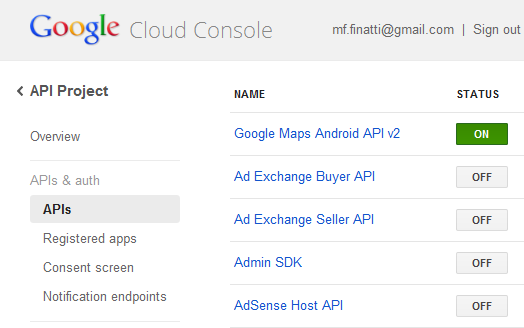
\includegraphics{figuras/api/localizacao/console1.png}
		  \caption{Ativando \emph{Maps API} no Google \emph{API Console}}
		  \label{fig:apiconsole1}
		\end{figure}

		Em seguida, é necessário registrar uma nova aplicação. Para isso, acesse \emph{Registered apps} no menu à esquerda e clique em \emph{REGISTER APP}. Preencha os campos de acordo e clique em \emph{Register}.

		\begin{figure}[H]
		  \centering
		  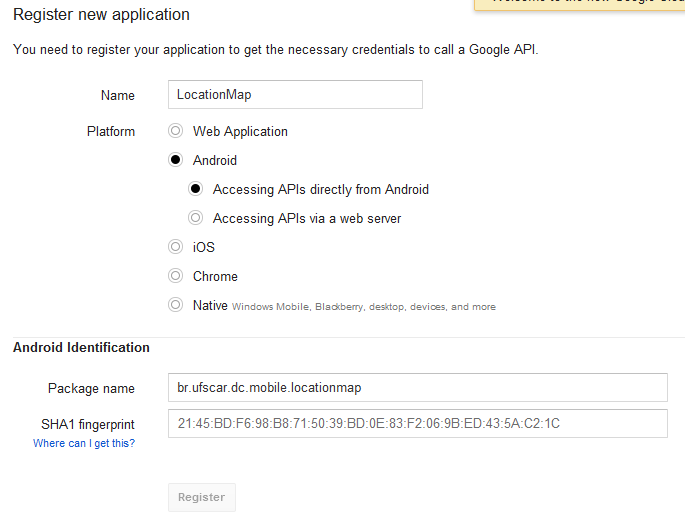
\includegraphics[width=.8\textwidth]{figuras/api/localizacao/console2.png}
		  \caption{Registrando um \emph{app} no Google \emph{API Console}}
		  \label{fig:apiconsole2}
		\end{figure}


		Com isso, você terá acesso a sua \emph{API Key} que será colocada no \emph{Manifest} para habilitar o uso do Google \emph{Maps} no dispositivo.
		
		\begin{figure}[H]
		  \centering
		  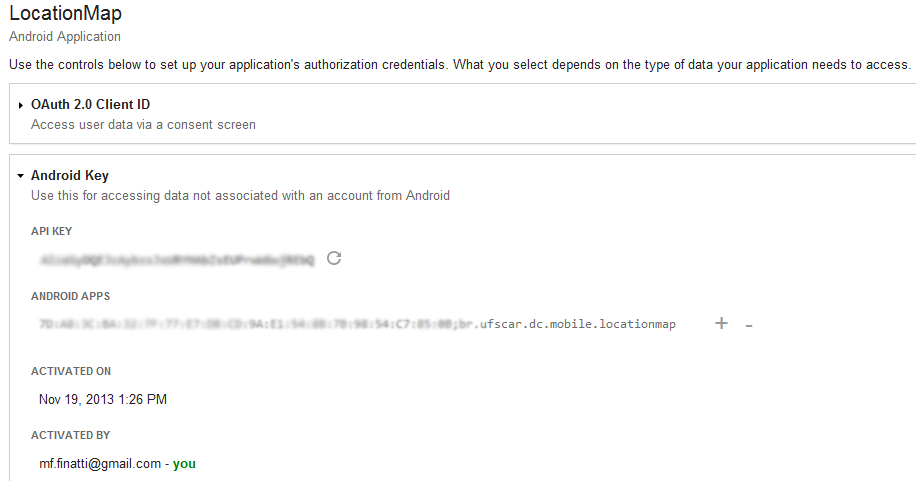
\includegraphics[width=.9\textwidth]{figuras/api/localizacao/console3.png}
		  \caption{Passo final para obter a \emph{API Key}}
		  \label{fig:apiconsole3}
		\end{figure}
	
		Agora, com o código em mãos, você deve abrir seu \emph{Manifest} e adicionar a seguinte linha dentro da \emph{tag} \texttt{<application>}. Onde \texttt{value} é a \emph{key} adquirida.

		\begin{listing}[H]
		\inputminted[linenos=true,fontsize=\small,frame=lines, framesep=2mm, tabsize=2,numbersep=5pt]{xml}{src/api/maps/apikey.xml}
		\caption{Configurando a \emph{API Key} no \emph{Manifest}}
		\label{code:apikey}
		\end{listing} 	

		\subsection{Configurando o Google  \emph{Play Services}}

		Primeiro, você deve fazer \emph{download} do Google \emph{Play Services} no \emph{SDK Manager}. Após o término do \emph{download} é necessário importar a biblioteca no Eclipse e referenciá-la em seu projeto. 
		
		A pasta com a biblioteca do Google \emph{Play Services} se encontrará na pasta \\ \texttt{sdk/extras/google/google\_play\_services/libproject/} e se chama \texttt{google-play-services\_lib}. É necessário importar essa pasta como projeto existente no Eclipse, não se esqueça de marcar a opção para copiar o projeto para o seu \emph{workspace}. 

		Depois de importar, você deve abrir as propriedades do seu projeto e selecionar \emph{Android} no menu à esquerda. Na parte inferior onde está escrito \emph{Library} clique em \emph{Add...} e selecione o \texttt{google-play-services\_lib}. Se aparecer um símbolo verde de "correto", então deu certo.

		\begin{figure}[H]
		  \centering
		  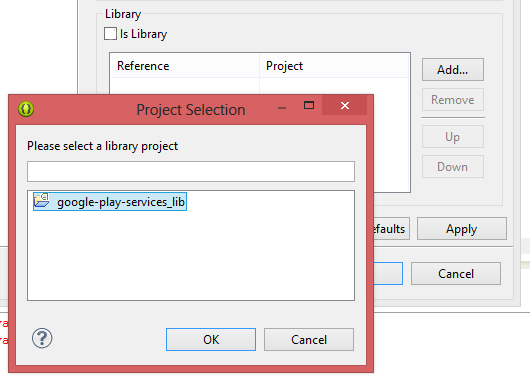
\includegraphics[width=.8\textwidth]{figuras/api/localizacao/playlib.png}
		  \caption{Adicionando a Google \emph{Play Services} como biblioteca do projeto}
		  \label{fig:apiplaylib}
		\end{figure}

		\subsection{Adicionando um mapa em sua \emph{activity}}

		O Google \emph{Maps} no Android usa OpenGL ES versão 2 para renderizar o mapa, logo é necessário adicionar o uso do OpenGL no \emph{Manifest}.

		\begin{listing}[H]
		\inputminted[linenos=true,fontsize=\small,frame=lines, framesep=2mm, tabsize=2,numbersep=5pt]{xml}{src/api/maps/opengl.xml}
		\caption{Adicionando o uso do OpenGL no \emph{Manifest}}
		\label{code:mapfrag}
		\end{listing} 	

		Agora que já obtemos a localização, podemos usá-la para marcar a posição no mapa. Existem diversas maneiras de adicionar um mapa em uma \emph{activity}. Nesse exemplo utilizaremos um \texttt{FrameLayout} para colocar o mapa dentro. Uma outra forma é simplesmente declarando um fragmento no XML do \emph{layout} como mostrado abaixo:

		\begin{listing}[H]
		\inputminted[linenos=true,fontsize=\small,frame=lines, framesep=2mm, tabsize=2,numbersep=5pt]{xml}{src/api/maps/frag.xml}
		\caption{Adicionando o mapa como um fragmento no XML}
		\label{code:mapfrag2}
		\end{listing} 	
		
		O \emph{layout} da \emph{activity} consiste de dois \texttt{TextView} para mostrar a latitude e a longitude do dispositivo no momento, alem disso tem um \texttt{FrameLayout} que irá conter o fragmento do mapa.

		\begin{listing}[H]
		\inputminted[linenos=true,fontsize=\small,frame=lines, framesep=2mm, tabsize=2,numbersep=5pt]{java}{src/api/maps/activity.java}
		\caption{\emph{Activity} com Google \emph{Maps}}
		\label{code:mapactivity}
		\end{listing} 	
		
		O primeiro detalhe a ser notado é que a \emph{Activity} está estendendo \texttt{FragmentActivity} a fim de poder usar o \texttt{SupportFragment} para compatibilidade com versões anteriores do Android. As linhas 18 a 22 já são conhecidas, do exemplo anterior. 

		Na linha 27 estamos usando \texttt{findFragmentByTag()} para podermos obter o fragmento do mapa, caso ele não esteja declarado no XML, será criada uma nova instância na linha 32. Na linha 34 a 38 estamos adicionando o fragmento do mapa ao \texttt{FrameLayout} do \emph{layout} usando \texttt{FragmentTransaction} e por fim chamando uma função \texttt{setUpMadIfNeeded()} para obtermos a instância do mapa (e não do seu fragmento). 

		\begin{listing}[H]
		\inputminted[linenos=true,fontsize=\small,frame=lines, framesep=2mm, tabsize=2,numbersep=5pt]{java}{src/api/maps/setupif.java}
		\caption{Método \texttt{setUpMapIfNeeded()}}
		\label{code:setupif}
		\end{listing} 	

		Apenas obtemos a instância do mapa de seu fragmento e criando um marcador na posição (0,0). Importante salientar que o principal motivo de se fazer esse método é para poder chamá-lo no método \texttt{onResume()} da \emph{activity} a fim de atualizar o mapa caso o aplicativo tenha sido parado por algum motivo. Agora iremos modificar o método \texttt{onLocationChanged()} do \texttt{MyLocationListener} para atualizar a posição no mapa e adicionar um marcador na posição correta.
		
		\begin{listing}[H]
		\inputminted[linenos=true,fontsize=\small,frame=lines, framesep=2mm, tabsize=2,numbersep=5pt]{java}{src/api/maps/onlocmod.java}
		\caption{Método \texttt{onLocationChanged()} modificado}
		\label{code:onlocmod}
		\end{listing} 	
		
		Primeiro removemos o marcador anterior, depois adicionamos um novo marcador na posição obtida pelo \emph{listener}. Na linha 13 chamamos o método \texttt{moveCamera()} para colocar a câmera na posição do marcador. 

		Para mais exemplos de mapas, você pode importar o projeto \emph{maps} da pasta \emph{samples} onde você obteve o \emph{libproject}.
	
%%%COMPARTILHAMENTO%%%
\chapter{Compartilhamento} 

		Já aprendemos a enviar dados à outras \emph{activities} usando a classe \texttt{Intent}. Agora veremos como faz para enviar esses dados e dar ao usuário a opção de escolher qual aplicativo já instalado no dispositivo ele quer usar para receber esses dados. Isso pode ser visto como compartilhamento. Imagine que você tirou uma foto e quer mostrar ao seus amigos pelo \emph{Facebook}. Na verdade está enviando uma foto à \emph{activity} do Facebook que recebe esse tipo de dado e assim ela tomará o controle.

		Quando você construir um \texttt{Intent} você deve especificar a ação que você espera que ele acione. O Android já define vários tipos de ações e entre eles está o \texttt{ACTION\_SEND} que indica que o \texttt{intent} está enviando dados de uma \emph{activity} para outra. 

		Se você quer enviar apenas um texto, por exemplo, basta seguir o pequeno exemplo abaixo:

		\begin{listing}[H]
		\inputminted[linenos=true,fontsize=\small,frame=lines, framesep=2mm, tabsize=2,numbersep=5pt]{java}{src/api/sharing/simpletext.java}
		\caption{Enviando um texto simples através de um \texttt{Intent}}
		\label{code:simpletext}
		\end{listing} 		

		Contanto que exista um aplicativo instalado no aparelho com um filtro que aceite \texttt{ACTION\_SEND} e o tipo \texttt{MIME} \texttt{"text/plain"} o Android irá executá-lo, caso exista mais de um então um alerta aparecerá perguntando qual aplicativo o usuário deseja escolher para receber o \texttt{Intent}. 

\begin{framed}
\paragraph{}\textbf{Dica}: Se chamar \texttt{Intent.createChooser()} então o Android sempre irá mostrar o alerta. Você pode configurar o texto a ser mostrado no parâmetro.
\textit{}
\end{framed}

		\begin{listing}[H]
		\inputminted[linenos=true,fontsize=\small,frame=lines, framesep=2mm, tabsize=2,numbersep=5pt]{java}{src/api/sharing/createchooser.java}
		\caption{Chamando \texttt{createChooser()}}
		\label{code:createchooser}
		\end{listing} 		

		Você pode usar alguns \emph{extras} padrões nos \texttt{Intent}, tais como: \texttt{EXTRA\_EMAIL} para o texto ser o corpo do e-mail, \texttt{EXTRA\_SUBJECT} para o texto ser o assunto do e-mail. Porém o aplicativo que estiver recebendo o \texttt{Intent} deve estar preparado para esse tipo de \emph{extra}, se não nada vai acontecer. Existe ainda a opção de criar \emph{extras} personalizados, mas também só irá funcionar caso o aplicativo esteja projetado para esse tipo de \emph{extra}. Nesse caso é comum criar um \emph{extra} personalizado caso você tenha feito um conjunto de aplicativos que podem trocar informações através de \texttt{Intents} e que irão usar esse \emph{extra}.

		Além de texto é possível enviar dados binários ou até mesmo mais de um dado ao enviar uma lista. Para enviar uma foto que você tirou com a câmera, por exemplo, você deve usar o \emph{extra} chamado \texttt{EXTRA\_STREAM} e configurar o tipo do \texttt{Intent} para \texttt{"image/jpeg"}.

		Uma forma mais completa de enviar imagens ou outros tipos de dados é usando um \\ \texttt{ContentProvider}\footnote{\href{http://developer.android.com/intl/es/reference/android/content/ContentProvider.html}{http://developer.android.com/intl/es/reference/android/content/ContentProvider.html}} que irá criar uma interface para a prover os dados a outras aplicações.

		Outra parte importante do compartilhamento é fazer com que sua aplicação consiga receber dados de \texttt{Intents}. O primeiro passo para isso é configurar os \texttt{intent-filter} no \emph{Manifest}. Quando você define um \texttt{intent-filter} você está dizendo para o Android que uma determinada \emph{activity} é capaz de receber um determinado de \texttt{Intent}. Uma \emph{activity} pode ter múltiplos filtros, cada um relacionado a um determinado tipo de dado.

		Para exemplificar o conceito, iremos fazer um aplicativo que escreve um texto e tira uma foto e um aplicativo que recebe um texto ou uma imagem e mostra o que foi recebido. O aplicativo usa conceitos já conhecidos então iremos nos limitar a explicar somente a parte do compartilhamento. Entretanto, caso haja dúvidas é possível obter ambos aplicativos do repositório.

		No primeiro aplicativo, é interessante salientar apenas os botões que adicionei para compartilhar. Um tem a função de compartilhar o texto e outro a imagem. Você pode, por exemplo compartilhar um e depois o outro no aplicativo do \emph{Gmail} que ambos irão ser adicionados ao corpo do e-mail.
		
		Observe no \hyperref[code:sharingbtn]{Algoritmo \ref*{code:sharingbtn}}, como ficaram os botões de compartilhamento.

		\begin{listing}[H]
		\inputminted[linenos=true,fontsize=\small,frame=lines, framesep=2mm, tabsize=2,numbersep=5pt]{java}{src/api/sharing/sharingbtn.java}
		\caption{Botões para compartilhar texto e imagem}
		\label{code:sharingbtn}
		\end{listing} 		

		A parte mais importante é o método \texttt{setType}, ele recebe um \emph{MIME Type}\footnote{MIME: \href{http://en.wikipedia.org/wiki/MIME}{http://en.wikipedia.org/wiki/MIME}}, como é o caso de \texttt{text/plain} e \texttt{image/png}. Outros \emph{MIME Types} poderiam ser usados como \texttt{image/*} caso não soubéssemos o formato da imagem ou até mesmo \texttt{*/*} que representa qualquer tipo de dado. O problema disso é que todos aplicativos irão aparecer na lista e alguns podem não receber o que você está tentando enviar! Portanto, seja cauteloso.

		Já o segundo aplicativo irá receber tanto um texto como uma foto e mostrar ao usuário, apenas para exemplificar o recebimento de \texttt{Intents}. O primeiro passo é criar os \texttt{intent-filter} para receber os \emph{MIME Type} corretos.

		\begin{listing}[H]
		\inputminted[linenos=true,fontsize=\small,frame=lines, framesep=2mm, tabsize=2,numbersep=5pt]{xml}{src/api/sharing/intentfilter.xml}
		\caption{Configurando os \texttt{intent-filter} no \emph{Manifest}}
		\label{code:intentfilter}
		\end{listing} 	

		É necessário criar um \texttt{intent-filter} para cada tipo de dado que será recebido. Como nesse caso só existe uma \emph{activity}, ela é tanto uma \emph{activity Launcher}, ou seja, aquela que abre o apicativo. Mas também recebe dois \emph{MIME Types}, são eles \texttt{text/plain} e \texttt{image/*}. Em seguida, precisamos receber os dados do \texttt{Intent} e mostrá-los para o usuário, como é feito no \hyperref[code:sharingintent]{Algoritmo \ref*{code:sharingintent}}:

		\begin{listing}[H]
		\inputminted[linenos=true,fontsize=\small,frame=lines, framesep=2mm, tabsize=2,numbersep=5pt]{java}{src/api/sharing/receive.java}
		\caption{Obtendo os dados do \texttt{Intent} e mostrando ao usuário}
		\label{code:sharingintent}
		\end{listing} 		

		Lembre-se que nesse trecho de código, estamos apenas preocupados em obter os dados do \texttt{Intent} e colocá-los nas suas \emph{views} e portanto não é o código completo da \emph{activity}. Basicamente o que fazemos é comparar as \emph{strings} recebidas no \texttt{Intent} para saber o que está sendo recebido. Ao verificar o \emph{action}, sabemos que o \texttt{Intent} veio através de compartilhamento e ao analisar o \emph{type}, sabemos o \emph{MIME type} e podemos construir a \emph{activity} de acordo.

\begin{framed}
\paragraph{}\textbf{Dica}: Modifique a \emph{activity} para salvar a imagem ou o texto no caso do usuário voltar para compartilhar outra coisa. Você pode salvar os dados no \texttt{Bundle}.
\textit{}
\end{framed}

		Esse capítulo tentou apenas para dar uma introdução ao compartilhamento de dados entre aplicativos. Outras coisas interessantes podem ser feitas, por exemplo adicionar o botão de \emph{Easy Share} como descrito \href{http://developer.android.com/intl/es/training/sharing/shareaction.html}{nessa página}\footnote{\href{http://developer.android.com/intl/es/training/sharing/shareaction.html}{http://developer.android.com/intl/es/training/sharing/shareaction.html}} da documentação. Além disso, existe também a classe \texttt{ContentProvider} que fornece uma interface para compartilhamento.

%%%AGENDA DE CONTATOS%%%		
\chapter{Agenda e Contatos} 
	\section{Usando o \emph{Contacts Provider}}

	O Android contém um repositório central onde estão armazenadas as informações dos contatos do usuário, incluindo os dados de redes sociais. Esse repositório se chama \emph{Contacts Provider}\footnote{\href{http://developer.android.com/guide/topics/providers/contacts-provider.html}{http://developer.android.com/guide/topics/providers/contacts-provider.html}}.	
	
	Seguindo as lições da documentação oficial, iremos criar uma pequena aplicação que obtém todos seus contatos e popula uma lista com eles. Mais detalhes do contato poderão ser obtidos ao se clicar no contato. O primeiro passo, sempre obrigatório para se acessar o repositório de contatos, é adicionar permissão no \emph{Manifest}. Demonstrado no trecho abaixo:	

		\begin{listing}[H]
		\inputminted[linenos=true,fontsize=\small,frame=lines, framesep=2mm, tabsize=2,numbersep=5pt]{xml}{src/api/contacts/permission.xml}
		\caption{Permissão para acessar os contatos}
		\label{code:contactpermission}
		\end{listing} 	
	
	Em seguida precisamos de uma \emph{activity} com uma lista para conter os contatos. Nesse exemplo criamos um XML de \emph{layout} que só contenha uma \texttt{ListView} e em seguida um outro XML para definir o \emph{layout} de um item da lista, nesse caso será somente uma \texttt{TextView}. Você poderá obter mais detalhes no código do projeto disponível no repositório.

\begin{framed}
\paragraph{}\textbf{Dica}: Você pode incrementar essa lista adicionando outras informações do contato na lista, como a foto de cada um.
\textit{}
\end{framed}

	Após ter definido o \emph{layout} precisamos mostrar a lista de contatos, comece definindo a \emph{activity} que irá conter a lista. A lista deverá ser populada utilizando a classe \texttt{ContactsContract}\footnote{\href{http://developer.android.com/reference/android/provider/ContactsContract.html}{http://developer.android.com/reference/android/provider/ContactsContract.html}} que já nos providencia algumas constantes e métodos para acessar a lista de contatos.

		\begin{listing}[H]
		\inputminted[linenos=true,fontsize=\small,frame=lines, framesep=2mm, tabsize=2,numbersep=5pt]{java}{src/api/contacts/fragment.java}
		\caption{\emph{Activity} que irá conter a lista de contatos}
		\label{code:contactfragment}
		\end{listing} 	
	
	Como pode ser observado no \hyperref[code:contactfragment]{Algoritmo \ref*{code:contactfragment}} estamos estendendo a classe \texttt{FragmentActivity}\footnote{\href{http://developer.android.com/reference/android/support/v4/app/FragmentActivity.html}{http://developer.android.com/reference/android/support/v4/app/FragmentActivity.html}} que nos permite usar o \texttt{Loader} em Android mais antigos. Além disso estamos implementando as interfaces \texttt{LoaderManager.LoaderCallbacks}\footnote{\href{http://developer.android.com/reference/android/app/LoaderManager.LoaderCallbacks.html}{http://developer.android.com/reference/android/app/LoaderManager.LoaderCallbacks.html}} que permite o carregamento de dados de forma assíncrona. Estamos implementando também a interface \texttt{OnItemClickListener}\footnote{\href{http://developer.android.com/reference/android/widget/AdapterView.OnItemClickListener.html}{http://developer.android.com/reference/android/widget/AdapterView.OnItemClickListener.html}} para que possamos carregar mais informações do contato quando este é clicado na lista.
	
	Precisamos de algumas variáveis para auxiliar na seleção dos contatos e na criação do adaptador da lista. A variável \texttt{FROM\_COLUMNS}, abaixo, são os dados que serão mostrados e que nesse caso é apenas o nome do contato. Observe que estamos fazendo uma pequena comparação da versão do SDK pois a partir da versão 3.0 do SDK, a classe \texttt{Contacts} foi alterada. Já a variável \texttt{TO\_IDS} serve para o adaptador saber onde colocar a informação, passamos para ele o \emph{id} do \texttt{TextView} que colocamos no XML. Como essa lição se baseia na lição da documentação oficial, estamos usando um dos \emph{ids} padrões do Android.

		\begin{listing}[H]
		\inputminted[linenos=true,fontsize=\small,frame=lines, framesep=2mm, tabsize=2,numbersep=5pt]{java}{src/api/contacts/fromto.java}
		\caption{Variáveis para o adaptador da lista}
		\label{code:contactadaptervar}
		\end{listing} 	

	As próximas variáveis são aquelas da seleção dos contatos. Nesse exemplo vamos obter todos os contatos e portanto deixar a variável \texttt{mSearchString} vazia, mas caso queira obter contatos específicos, basta fazer algo que preencha essa variável. Temos a variável \texttt{SELECTION} que funciona como a parte \emph{WHERE} de uma consulta \texttt{SQL}, ela já está preparada para a busca por algum nome, caso queira. A variável \texttt{PROJECTION} é uma constante que define as colunas que você quer retornar das consultas, nesse caso queremos 3: o \emph{id} do contato, sua chave de busca \emph{(lookup key)} e o seu nome. Por fim, as variáveis \texttt{CONTACT\_ID\_INDEX} e \texttt{LOOKUP\_KEY\_INDEX} funcionam como ponteiros para o \texttt{Cursor} que irá se mover nos resultados da pesquisa, basta definir o valor da variável como sendo a posição da coluna na projeção. Como temos a coluna \emph{id} sendo a primeira e a \emph{lookup} sendo a segunda, colocamos os valores 0 e 1, respectivamente. Isso é necessário para se obter dados de uma coluna individual do \texttt{Cursor}.

		\begin{listing}[H]
		\inputminted[linenos=true,fontsize=\small,frame=lines, framesep=2mm, tabsize=2,numbersep=5pt]{java}{src/api/contacts/morevar.java}
		\caption{Variáveis para o \texttt{Cursor} do conjunto resultante da busca}
		\label{code:contactcursorvar}
		\end{listing} 	

	As últimas variáveis de que precisamos são estas, para armazenar os resultados da consulta e guardar referências. Iremos usar a \texttt{Uri} do contato para buscar mais informações posteriormente.

		\begin{listing}[H]
		\inputminted[linenos=true,fontsize=\small,frame=lines, framesep=2mm, tabsize=2,numbersep=5pt]{java}{src/api/contacts/lastvar.java}
		\caption{Variáveis de controle}
		\label{code:contactlastvar}
		\end{listing} 	

	Depois, precisamos implementar o método \texttt{onCreate()}. Nesse método, iremos configurar o adaptador da lista que será um \texttt{SimpleCursorAdapter}\footnote{\href{http://developer.android.com/reference/android/widget/SimpleCursorAdapter.html}{http://developer.android.com/reference/android/widget/SimpleCursorAdapter.html}}. Esse adaptador liga os resultados da busca com a \texttt{ListView}.

		\begin{listing}[H]
		\inputminted[linenos=true,fontsize=\small,frame=lines, framesep=2mm, tabsize=2,numbersep=5pt]{java}{src/api/contacts/onactivity.java}
		\caption{Método \texttt{onActivityCreated()}}
		\label{code:contactonactivity}
		\end{listing} 	

	Na linha 4 do \hyperref[code:contactonactivity]{Algoritmo \ref*{code:contactonactivity}}, estamos criando o \texttt{SimpleCursorAdapter}, como já discutido na lição de listas, é necessário passar para o adaptador o \emph{layout} interno da lista assim como os mapas com os dados e os \emph{ids} das \emph{views} em que esses dados serão inseridos. São esses parâmetros as variáveis \texttt{FROM\_COLUMNS} e \texttt{TO\_IDS}. Na linha 10 determinamos o adaptador para a lista e na linha 11 determinamos que o listener da lista será a própria classe. Isso é possível pois estamos implementando a interface \texttt{OnItemClickListener}.

	Como estamos usando o \texttt{CursorLoader}\footnote{\href{http://developer.android.com/reference/android/content/CursorLoader.html}{http://developer.android.com/reference/android/content/CursorLoader.html}} para buscar os dados, nós precisamos inicializar a \emph{thread} que ficará no plano de fundo que irá controlar a busca de forma assíncrona. 

	O próximo passo é implementar o método \texttt{onCreateLoader()}, que irá realizar a consulta, ao retornar um \texttt{CursorLoader} que recebeu como parâmetros da busca .

		\begin{listing}[H]
		\inputminted[linenos=true,fontsize=\small,frame=lines, framesep=2mm, tabsize=2,numbersep=5pt]{java}{src/api/contacts/oncreateloader.java}
		\caption{Método \texttt{onCreateLoader()}}
		\label{code:contactoncreateloader}
		\end{listing} 	

	Depois, você deve implementar os métodos \texttt{onLoadFinished()} e \texttt{onLoaderReset()}. O primeiro é chamado quando o \emph{Contacts Provider} retorna os resultados da consulta, usamos o método \texttt{swapCursor()} para trocar o \emph{cursor} do adaptador pelo \emph{cursor} do método \texttt{onLoadFinished()}. Já o segundo é chamado quando o \emph{framework} detecta que o \emph{cursor} contém dados desatualizados, nesse caso basta apagar a referência ao \emph{cursor} no adaptador.
	 
	Por fim, você deve implementar o método \texttt{onItemClick()} para abrir uma nova \emph{activity} ao clicar no contato.

		\begin{listing}[H]
		\inputminted[linenos=true,fontsize=\small,frame=lines, framesep=2mm, tabsize=2,numbersep=5pt]{java}{src/api/contacts/onitemclick.java}
		\caption{Método \texttt{onItemClick()}}
		\label{code:contactonitemclick}
		\end{listing} 	
			
	Primeiro nós obtemos a posição na lista através do parâmetro \texttt{position}, em seguida colocamos o \emph{cursor} nessa posição e obtemos os dados do contato. Usando o método \texttt{getLookupUri()} nós conseguimos a \texttt{URI} do contato para que seja possível acessar suas informações detalhadas.

	\subsection{Detalhes de um contato}

	Conseguir os detalhes do contato usa o mesmo princípio de conseguir todos os contatos. Devemos fazer algumas consultas, mas com seleções e projeções diferentes. Para obter os telefones de um contato, deverá acessar o campo \emph{Phone} do \texttt{ContactsContract}, para obter os e-mails: \emph{Email}, e para acessar os endereços: \emph{StructuredPostal}.

	Nesse exemplo, criaremos uma nova \emph{activity} que irá conter os dados do contato escolhido na primeira \emph{activity}. Para facilitar a leitura do código, iremos criar três interfaces para serem usadas, essas interfaces irão conter as projeções e seleções de cada um dos tipos de dado. 

		\begin{listing}[H]
		\inputminted[linenos=true,fontsize=\small,frame=lines, framesep=2mm, tabsize=2,numbersep=5pt]{java}{src/api/contacts/interfaces.java}
		\caption{Interfaces das consultas dos contatos}
		\label{code:contactinterfaces}
		\end{listing} 	

	Dessa forma, mostrada no \hyperref[code:contactinterfaces]{Algoritmo \ref*{code:contactinterfaces}}, conseguimos organizar melhor o código para as consultas que iremos fazer. Essa \emph{activity}, que decidi chamar \texttt{ContactDetailsActivity} também irá estender \texttt{FragmentActivity} e implementar \texttt{LoaderCallbacks<Cursor>}. Iremos utilizar essas três variáveis, das quais duas serão obtidas do \texttt{Intent} que abriu essa \emph{activity}.
	
		\begin{listing}[H]
		\inputminted[linenos=true,fontsize=\small,frame=lines, framesep=2mm, tabsize=2,numbersep=5pt]{java}{src/api/contacts/contactdetails.java}
		\caption{Classe \texttt{ContactDetailsActivity}}
		\label{code:contactdetailsactivity}
		\end{listing} 	


	Em seguida, construa o método \texttt{onCreate()}. A diferença dessa \emph{activity} para a anterior é a obtenção dos dados do \texttt{Intent} e a referência ao \texttt{ViewGroup} que iremos utilizar mais tarde. 

		\begin{listing}[H]
		\inputminted[linenos=true,fontsize=\small,frame=lines, framesep=2mm, tabsize=2,numbersep=5pt]{java}{src/api/contacts/oncreate.java}
		\caption{Método \texttt{onCreate()} de \texttt{ContactDetailsActivity}}
		\label{code:contactdetailsoncreate}
		\end{listing} 	

	O método \texttt{setContact()} é usado para colocar os dados obtidos do \texttt{Intent} nos atributos da classe e chamar as consultas necessárias. Chamamos o método \texttt{restartLoader()} para forçar a criação da \emph{thread} que irá realizar a consulta. Observe que cada uma é responsável por uma consulta, passamos o \texttt{QUERY\_ID} de cada uma das interfaces para diferenciá-las.

		\begin{listing}[H]
		\inputminted[linenos=true,fontsize=\small,frame=lines, framesep=2mm, tabsize=2,numbersep=5pt]{java}{src/api/contacts/setcontact.java}
		\caption{Método \texttt{setContact()}}
		\label{code:contactdetailssetcontact}
		\end{listing} 			
		\interfootnotelinepenalty=10000
	O método \texttt{hasPhone()}, chamado na linha 14, verifica se o contato tem algum número de telefone cadastrado. Esse método demonstra uma outra forma de se adquirir os dados de um contato, sem ser em outra \emph{thread}, mas na mesma \emph{thread} da \emph{UI (User Interface)}\footnote{Tudo que fizemos até agora (exceto o \texttt{AsyncTask} na lição de comunicação) está rodando na chamada \emph{UI thread}, isso significa que o Android está executando seu código na mesma \emph{thread} em que cria a interface do usuário. Usar o \texttt{Loader} implica em fazer com que as consultas rodem em uma outra \emph{thread}, liberando a \emph{UI thread} do serviço e impedindo que o aplicativo pareça estar travado enquanto busca informações. O \texttt{AsyncTask} é uma outra forma de executar \emph{background threads} de forma assíncrona.}. 

	
	Agora iremos implementar o método \texttt{onCreateLoader()}, de forma semelhante à última vez, mas agora iremos criar um \texttt{CursorLoader} diferente dependendo do \emph{id} que foi passado para o método - no caso é o \texttt{QUERY\_ID} que foi o parâmetro do método \texttt{restartLoader()}, visto no algoritmo \hyperref[code:contactdetailssetcontact]{Algoritmo \ref*{code:contactdetailssetcontact}}.
		
		 \begin{listing}[H]
		\inputminted[linenos=true,fontsize=\small,frame=lines, framesep=2mm, tabsize=2,numbersep=5pt]{java}{src/api/contacts/oncreateloader2.java}
		\caption{Método \texttt{onCreateLoader()}}
		\label{code:contactdetailssoncreateloader}
		\end{listing} 			
	
	Nesse método, nós estamos fazendo um \texttt{switch} para selecionar qual consulta iremos fazer e então usamos as projeções e seleções de cada interface para realizar a consulta. Se atente as diferenças entre cada um: no primeiro caso, nós usamos \texttt{mContactUri} no segundo parâmetro do construtor do \texttt{CursorLoader} pois nós já temos o "endereço" do nome do contato nesse atributo, nesse caso não é preciso fazer uma seleção.

	 No segundo e terceiro casos, no segundo parâmetro passamos o "endereço" da tabela dos endereços e telefones dos contatos, mas usamos a seleção para poder selecionar qual contato. A variável \texttt{addressArgs} contém o \emph{id} do contato que irá servir como parâmetro da seleção. Note que no Android essas informações dos contatos estão guardadas em um banco de dados e o que estamos fazendo na realidade são \emph{SELECT} comuns, mas usando as classes pré-definidas para nos auxiliar. O Android também já junta várias tabelas automaticamente para facilitar as buscas.

	Para finalizar, vamos implementar o método \texttt{onLoadFinished()}, nesse método é que adquirimos os dados do \texttt{cursor} e criamos as \emph{views} para mostrar esses dados. 

		 \begin{listing}[H]
		\inputminted[linenos=true,fontsize=\small,frame=lines, framesep=2mm, tabsize=2,numbersep=5pt]{java}{src/api/contacts/onloadfinished2.java}
		\caption{Método \texttt{onLoadFinished()}}
		\label{code:contactsdetailsonloadfinished}
		\end{listing} 			

		Novamente, o método irá tomar uma ação diferente dependendo de qual consulta foi realizada. Se existe um resultado, então nós criado uma \texttt{TextView} e colocamos o texto adquirido nela. Aqui é que usamos a variável \texttt{container}, usamos o método \texttt{addView()} para colocar essa \emph{view} dentro dela.

	
		Esse capítulo tentou dar uma introdução à obtenção dos contatos da agenda. É uma tema especialmente difícil por haver muito rigor nos detalhes. É altamente recomendável estudar mais a fundo a lição presente na documentação oficial e o exemplo oferecido por eles. 


\chapter{Acelerômetro}
	Os dispositivos Android contam com um sensor chamado acelerômetro que consegue captar a aceleração do aparelho nos três eixos. É útil para fazer jogos, saber a orientação do aparelho, entre outras utilidades. Para isso o Android contém um \emph{framework} para os sensores, uma das classes é a \texttt{SensorManager} que contém vários métodos para acessar, registrar \emph{listeners} e constantes para calibrar os sensores, reportar a precisão do sensor e configurar a taxa de aquisição dos dados. Para saber mais sobre o \emph{framework}, acesse a \href{http://developer.android.com/guide/topics/sensors/sensors\_overview.html}{documentação oficial}\footnote{\href{http://developer.android.com/guide/topics/sensors/sensors\_overview.html}{http://developer.android.com/guide/topics/sensors/sensors\_overview.html}}.

	Agora, para exemplificar vamos construir uma aplicação bem simples que apenas irá mostrar na tela os valores lidos do acelerômetro. Criaremos apenas uma \emph{activity} com três \texttt{TextView} para mostrar os valores lidos do acelerômetro.

	\begin{listing}[H]
	\inputminted[linenos=true,fontsize=\small,frame=lines, framesep=2mm, tabsize=2,numbersep=5pt]{java}{src/api/accelerometer/activity.java}
	\caption{Classe \texttt{AccelActivity}}
	\label{code:accelactivity}
	\end{listing} 			

	Usaremos os dois \emph{arrays}, \texttt{gravity} e \texttt{acceleration} para guardar os valores lidos do sensor. Em seguida, no método \texttt{onCreate()}, você deverá adquirir uma referência do \texttt{SensorManager} usando \texttt{getSystemService()}.

	\begin{listing}[H]
	\inputminted[linenos=true,fontsize=\small,frame=lines, framesep=2mm, tabsize=2,numbersep=5pt]{java}{src/api/accelerometer/oncreate.java}
	\caption{Método \texttt{onCreate()} de \texttt{AccelActivity}}
	\label{code:accelactivitycreate}
	\end{listing} 			

	É necessário agora criar o \emph{listener} que irá escutar o sensor e escrever os dados na tela. O método \texttt{onSensorChanged()} é chamado de acordo com o intervalo definido em \\ \texttt{registerListener()} na linha 4 do algoritmo \hyperref[code:accelregister]{Algoritmo \ref*{code:accelregister}}.

	\begin{listing}[H]
	\inputminted[linenos=true,fontsize=\small,frame=lines, framesep=2mm, tabsize=2,numbersep=5pt]{java}{src/api/accelerometer/listener.java}
	\caption{Método \texttt{onSensorChanged()}}
	\label{code:accelonsensorchanged}
	\end{listing} 			
	
	Primeiro verificamos se o sensor que chamou o método é o acelerômetro, só prosseguimos caso seja. Os dados lidos estão armazenados no \emph{array} \texttt{event}. Cada índice indica um eixo: 0 é o eixo X, 1 é o eixo Y e 2 é o eixo Z. Para calcular corretamente a aceleração, precisamos retirar o componente gravitacional da conta. Para isso fazemos um filtro passa-baixo, como indicado na documentação\footnote{\href{http://developer.android.com/guide/topics/sensors/sensors\_motion.html}{http://developer.android.com/guide/topics/sensors/sensors\_motion.html}}.

	Por último, deve-se registrar o \emph{listener} quando a \emph{activity} está em primeiro plano e desregistrar quando a \emph{activity} for pausada. Isso é necessário para não ficar consumindo a bateria de forma desnecessária. Logo, será necessário fazer isso nos métodos \texttt{onResume()} e \texttt{onPause()}.

	\begin{listing}[H]
	\inputminted[linenos=true,fontsize=\small,frame=lines, framesep=2mm, tabsize=2,numbersep=5pt]{java}{src/api/accelerometer/register.java}
	\caption{Métodos \texttt{onResume()} e \texttt{onPause()}}
	\label{code:accelregister}
	\end{listing} 			

	Quando registrar o \emph{listener}, é importante indicar o intervalo de atualização (terceiro parâmetro), estamos usando \texttt{SENSOR\_DELAY\_NORMAL} pois é o mais lento. 
	
	Esse capítulo buscou apenas dar uma introdução bem simples ao uso de sensores, mas mais especificamente ao uso do acelerômetro. Todos os sensores podem ser programados de forma similar. 

%%%BLUETOOTH%%%
\chapter{Bluetooth}

	O Android providencia uma API para conectar o aparelho em outros dispositivos \emph{Bluetooth}, sejam outros celulares, \emph{tablets}, fones de ouvido e até mesmo HDP \emph{(Health Device Profile)} que é um tipo de conexão \emph{Bluetooth} para aparelhos médicos. Com a API para \emph{Bluetooth} você pode: sondar outros dispositivos \emph{Bluetooth}, buscar por dispositivos já pareados, estabelecer conexões, transferir dados e gerenciar múltiplas conexões.

	Para exemplificar iremos construir uma pequena aplicação que envia uma mensagem para um dispositivo pareado. Esse exemplo irá introduzir diversos novos conceitos do sistema Android e do próprio Java, entre eles: \texttt{BroadcastReceiver}, \texttt{Thread}, \texttt{Handler}, \texttt{Runnable}, além claro, do \texttt{Bluetooth}.
 
	 Primeiro nossa aplicação deve recuperar todos os dispositivos \emph{bluetooth} já conhecidos, ou seja, aqueles que já foram pareados com o nosso aparelho. Colocaremos numa \texttt{ListView} tanto os dispositivos pareados como aqueles novos que iremos procurar. 

	Iniciaremos com uma classe que chamei de \texttt{DeviceListActivity}, essa \emph{activity} irá mostrar a lista dos dispositivos encontrados, ao se clicar em um desses dispositivos, uma mensagem será enviada através de um \emph{socket}. Somente se o outro dispositivo estiver rodando a aplicação no mesmo momento é que a mensagem poderá ser visualizada.

	\begin{listing}[H]
	\inputminted[linenos=true,fontsize=\small,frame=lines, framesep=2mm, tabsize=2,numbersep=5pt]{java}{src/api/bluetooth/activity.java}
	\caption{Classe \texttt{DeviceListActivity}}
	\label{code:bluetooth-activity}
	\end{listing} 			

	Usaremos um \texttt{ArrayAdapter}\footnote{\href{http://developer.android.com/reference/android/widget/ArrayAdapter.html}{http://developer.android.com/reference/android/widget/ArrayAdapter.html}} para mostrar na lista o nome e o endereço MAC dos dispositivos. Além disso, a variável \texttt{BluetoothAdapter}\footnote{\href{http://developer.android.com/reference/android/bluetooth/BluetoothAdapter.html}{http://developer.android.com/reference/android/bluetooth/BluetoothAdapter.html}} é usada para iniciar a varredura por novos dispositivos, obter a lista de dispositivos pareados instanciar um \texttt{BluetoothDevice}\footnote{\href{http://developer.android.com/reference/android/bluetooth/BluetoothDevice.html}{http://developer.android.com/reference/android/bluetooth/BluetoothDevice.html}} e criar um \texttt{BluetoothServerSocket}\footnote{\href{http://developer.android.com/reference/android/bluetooth/BluetoothServerSocket.html}{http://developer.android.com/reference/android/bluetooth/BluetoothServerSocket.html}} que irá aceitar novas conexões. 

	Agora já iremos para o método \texttt{onCreate()}, nesse método quatro importantes passos deverão ser seguidos. Os três primeiros estão sendo mostrados no código abaixo.

	\begin{listing}[H]
	\inputminted[linenos=true,fontsize=\small,frame=lines, framesep=2mm, tabsize=2,numbersep=5pt]{java}{src/api/bluetooth/oncreate1.java}
	\caption{Primeira parte do método \texttt{onCreate()}}
	\label{code:bluetooth-oncreate1}
	\end{listing} 			

	O primeiro passo, marcado na linha 6, é obter a referência do adaptador \emph{bluetooth} com a chamada ao método \texttt{BluetoothAdapter.getDefaultAdapter()}. Caso esse método retorne \texttt{null} então o aparelho Android não tem \emph{hardware Bluetooth} e, portanto, a aplicação não irá funcionar. 

	O segundo passo é verificar se o \emph{Bluetooth} está ativado, essa verificação é feita com uma chamada ao método \texttt{isEnabled()} como é feito na linha 13. Se o retorno for falso então nós iremos perguntar ao usuário se ele gostaria de ativar o adaptador \emph{Bluetooth}. Para isso é necessário lançar um \texttt{Intent} com \emph{action} igual à \texttt{BluetoothAdapter.ACTION\_REQUEST\_ENABLE}. Ao chamar o método \texttt{startActivityForResult()} um alerta irá perguntar ao usuário se ele quer ativar o \emph{Bluetooth}. A variável \texttt{REQUEST\_ENABLE\_BT} pode ser qualquer valor maior que 0.  

	O terceiro passo é obter todos os dispositivos já pareados, a classe \texttt{BluetoothAdapter} mantém uma lista desses dispositivos que pode ser adquirida com a chamada ao método \\ \texttt{getBondedDevices()}. Depois, adicionaremos o nome e endereço MAC desses dispositivos pareados à \texttt{ListView} usando o \texttt{ArrayAdapter}. 

	O método \texttt{onActivityResult()} não precisa de nada especial. Mostrar para o usuário um \emph{feedback} já é suficiente.

	\begin{listing}[H]
	\inputminted[linenos=true,fontsize=\small,frame=lines, framesep=2mm, tabsize=2,numbersep=5pt]{java}{src/api/bluetooth/onactivityresult.java}
	\caption{Método \texttt{onActivityResult()}}
	\label{code:bluetooth-onactivityresult}
	\end{listing} 			

	Voltando ao método \texttt{onCreate()} Observe o comentário \texttt{[1]} na linha 31 do \hyperref[code:bluetooth-oncreate1]{Algoritmo \ref*{code:bluetooth-oncreate1}}, nesse pedaço do código iremos adicionar um rodapé na \texttt{ListView} com um botão que iniciará a varredura por novos dispositivos.

	Apesar de não ter apresentado este conceito antes, rodapés e cabeçalhos em \texttt{ListViews} são bem simples, construa um \emph{layout} XML e use o \texttt{LayoutInflater} para obter a \texttt{View}, depois adicione essa \texttt{View} à lista usando \texttt{addFooterView()}. Rodapés e cabeçalhos precisam ser adicionados à \texttt{ListView} antes de definir o adaptador. Também adicionaremos um \emph{listener} a um botão para que ele inicie a varredura. O método \texttt{startDiscovery()} é usado para fazer a varredura.

	\begin{listing}[H]
	\inputminted[linenos=true,fontsize=\small,frame=lines, framesep=2mm, tabsize=2,numbersep=5pt]{java}{src/api/bluetooth/oncreate2.java}
	\caption{Segunda parte do método \texttt{onCreate()}}
	\label{code:bluetooth-oncreate2}
	\end{listing} 			

	Porém, chamar \texttt{startDiscovery()} não é suficiente, é necessário construir um \\ \texttt{BroadcastReceiver} para capturar os \texttt{Intents} que tenham as informações dos dispositivos \emph{Bluetooth} que foram descobertos.

	\begin{listing}[H]
	\inputminted[linenos=true,fontsize=\small,frame=lines, framesep=2mm, tabsize=2,numbersep=5pt]{java}{src/api/bluetooth/broadcast.java}
	\caption{\texttt{BroadcastReceiver} que captura dispositivos \emph{Bluetooth}}
	\label{code:bluetooth-broadcastreceiver}
	\end{listing} 			

	O que esse \texttt{BroadcastReceiver} está fazendo é capturar os \texttt{Intents} e verificar em quais deles o campo \emph{action} equivale a \texttt{BluetoothDevice.ACTION\_FOUND}. Sendo positivo, é obtido um \texttt{BluetoothDevice} que veio no campo \emph{extra} do \texttt{Intent}. Então repetimos o procedimento de adicionar esse dispositivo no adaptador da lista. É necessário criar um \texttt{IntentFilter}\footnote{\href{http://developer.android.com/reference/android/content/IntentFilter.html}{http://developer.android.com/reference/android/content/IntentFilter.html}} para ser usado com o \texttt{BroadcastReceiver}.

	Porém, para o \texttt{BroadcastReceiver} começar a funcionar é necessário registrá-lo com o método \texttt{registerReceiver()}. É importante também remove-lo com o método \\ \texttt{unregisterReceiver()} no método \texttt{onDestroy()}.

	\begin{listing}[H]
	\inputminted[linenos=true,fontsize=\small,frame=lines, framesep=2mm, tabsize=2,numbersep=5pt]{java}{src/api/bluetooth/register.java}
	\caption{Registrando e removendo o \texttt{BroadcastRegister}}
	\label{code:bluetooth-registerbroadcast}
	\end{listing} 			

	Agora, iremos criar três \emph{threads}. A primeira, chamada de \texttt{AcceptThread} será responsável por instanciar um \texttt{BluetoothSocketServer} e aceitar uma nova conexão vinda de um outro dispositivo. A segunda, \texttt{ConnectThread} será usada quando a aplicação funcionar como cliente, essa \emph{thread} irá tentar estabelecer uma conexão com outro dispositivo. Já a terceira, \texttt{ConnectedThread} será usada em ambos os casos, para gerenciar a conexão e a entrada e saída de dados. Todas essas \emph{threads} estão escritas como classes \emph{inline} (dentro da classe \texttt{DeviceListActivity}).

	A primeira \emph{thread}, \texttt{AcceptThread}, irá instanciar um \texttt{BluetoothServerSocket}\footnote{\href{http://developer.android.com/reference/android/bluetooth/BluetoothServerSocket.html}{http://developer.android.com/reference/android/bluetooth/BluetoothServerSocket.html}}  usando o método \texttt{listenUsingRfcommWithServiceRecord()}, esse método cria um \emph{socket} seguro em um canal \emph{Bluetooth}, portanto toda informação será criptografada. Os parâmetros são \texttt{name} e \texttt{uuid}, \texttt{name} é o nome do serviço que nesse caso pode ser qualquer coisa. Já o \texttt{uuid} é um identificador universal único para ser usado com a aplicação, pode-se obter um número usando geradores aleatórios de UUID disponíveis na \emph{web}. A \emph{thread} irá ficar tentando escutar uma conexão com o método \texttt{accept()}. Note que este método é bloqueante e irá retornar um \emph{socket} se a conexão foi aceita ou irá gerar uma exceção.
Como não queremos aceitar mais nenhuma conexão, chamamos \texttt{close()} que irá fechar o \texttt{BluetoothServerSocket} mas não irá fechar o \texttt{BluetoothSocket} criado, mantendo a conexão.

Se o \emph{socket} conseguir ser instanciado corretamente, iremos chamar o método \\ \texttt{manageConnection()}, responsável por instanciar a \emph{thread} que gerencia a conexão. 

	\begin{listing}[H]
	\inputminted[linenos=true,fontsize=\small,frame=lines, framesep=2mm, tabsize=2,numbersep=5pt]{java}{src/api/bluetooth/acceptthread.java}
	\caption{Classe \texttt{AcceptThread}}
	\label{code:bluetooth-acceptthread}
	\end{listing} 			

	O \hyperref[code:bluetooth-connectthread]{Algoritmo \ref*{code:bluetooth-connectthread}} abaixo mostra a segunda \emph{thread}, essa \emph{thread} é responsável por estabelecer uma conexão com outro dispositivo que esteja rodando a mesma aplicação, por isso é usado o mesmo UUID. O construtor irá receber um \texttt{BluetoothDevice}, que foi selecionado da lista, e tentará criar a conexão com o método \texttt{createRfcommSocketToServiceRecord()}. A \emph{thread} irá cancelar a varredura e irá tentar conectar ao socket usando \texttt{connect()}, que também é uma chamada bloqueante. Se a conexão falhar ou ocorrer um \emph{timeout}, ele irá gerar uma exceção. Por segurança, chamamos \texttt{close()} dentro do bloco \texttt{catch} para tentar fechar o \emph{socket} e liberar os recursos do aparelho. Se tudo der certo, chamamos o método \texttt{manageConnection()} que veremos logo. Por enquanto deixaremos a explicação da linha 29 em espera, voltaremos logo nela.

	\begin{listing}[H]
	\inputminted[linenos=true,fontsize=\small,frame=lines, framesep=2mm, tabsize=2,numbersep=5pt]{java}{src/api/bluetooth/connectthread.java}
	\caption{Classe \texttt{ConnectThread}}
	\label{code:bluetooth-connectthread}
	\end{listing} 	

	O método \texttt{manageConnection()} apenas irá instanciar a \emph{thread} \texttt{ConnectedThread}.

	\begin{listing}[H]
	\inputminted[linenos=true,fontsize=\small,frame=lines, framesep=2mm, tabsize=2,numbersep=5pt]{java}{src/api/bluetooth/manage.java}
	\caption{Método \texttt{manageConnection()}}
	\label{code:bluetooth-manage}
	\end{listing} 	

	Agora veremos a última \emph{thread}, essa resposável pela entrada e saída de dados através do \emph{socket}.

	\begin{listing}[H]
	\inputminted[linenos=true,fontsize=\small,frame=lines, framesep=2mm, tabsize=2,numbersep=5pt]{java}{src/api/bluetooth/connected.java}
	\caption{Classe \texttt{ConnectedThread}}
	\label{code:bluetooth-connected}
	\end{listing} 	

	Primeiro obtemos o \texttt{InputStream} e \texttt{OutputStream} do \emph{socket} usando os métodos \texttt{getInputStream()} e \texttt{getOutputStream()}, respectivamente. Você pode ler e escrever o fluxo de dados usando \texttt{read()} e \texttt{write()}, é necessário fazer isso numa \emph{thread} pois essas chamadas são bloqueantes. O método \texttt{read()} irá bloquear enquanto não houver nada para ler e o método \texttt{write()} pode bloquear caso o outro lado esteja lendo os \emph{buffers} muito lentamente. 

	A \emph{thread} irá repetir enquanto não houver exceção e ficará tentando ler do \emph{stream} usando \texttt{read()}. Aqui novamente colocaremos a explicação da linha 28 em espera e voltaremos nela posteriormente. Faremos também um método \texttt{write()} para essa classe, para embrulhar o método do \emph{socket}, que poderá ser chamado da \emph{activity}.

	Agora temos dois métodos, um para receber e mostrar a mensagem e outro para enviar a mensagem. O método \texttt{writeMessage()}, abaixo, abre um alerta com um \texttt{EditText} em que o usuário pode escrever a mensagem para ser enviada.

	\begin{listing}[H]
	\inputminted[linenos=true,fontsize=\small,frame=lines, framesep=2mm, tabsize=2,numbersep=5pt]{java}{src/api/bluetooth/writemessage.java}
	\caption{Método \texttt{writeMessage()}}
	\label{code:bluetooth-writemessage}
	\end{listing} 	
	 
	O método \texttt{showMessage()} mostra a mensagem recebida em um \texttt{Toast}.

	\begin{listing}[H]
	\inputminted[linenos=true,fontsize=\small,frame=lines, framesep=2mm, tabsize=2,numbersep=5pt]{java}{src/api/bluetooth/showmessage.java}
	\caption{Método \texttt{showMessage()}}
	\label{code:bluetooth-showmessage}
	\end{listing} 	

	Com isso, podemos voltar e explicar a linha 29 do \hyperref[code:bluetooth-acceptthread]{Algoritmo \ref*{code:bluetooth-acceptthread}} e a linha 28 do algoritmo \hyperref[code:bluetooth-connected]{Algoritmo \ref*{code:bluetooth-connected}}. Essas são chamadas para o \texttt{Handler} da \emph{UI thread}. Dessa forma, podemos chamar métodos que precisam estar na \emph{UI thread}, mas fora dela. A chamada irá esperar até que a \emph{UI thread} entre para executar.

	\begin{listing}[H]
	\inputminted[linenos=true,fontsize=\small,frame=lines, framesep=2mm, tabsize=2,numbersep=5pt]{java}{src/api/bluetooth/handler.java}
	\caption{\texttt{Handler} e \texttt{Runnable}}
	\label{code:bluetooth-handler}
	\end{listing} 	

	Os \texttt{Runnable} estão encarregados de executar os dois métodos, para mostrar e enviar a mensagem. O \texttt{Handler} irá chamar o \texttt{Runnable} quando estiver na \emph{UI thread}.

	Agora é necessário implementar o método \texttt{onItemClick()} para abrir a conexão com o dispositivo selecionado.

	\begin{listing}[H]
	\inputminted[linenos=true,fontsize=\small,frame=lines, framesep=2mm, tabsize=2,numbersep=5pt]{java}{src/api/bluetooth/onitemclick.java}
	\caption{Implementação do método \texttt{onItemClick()}}
	\label{code:bluetooth-onitemclick}
	\end{listing} 	

	Obtemos a \emph{string} do adaptador e usamos \texttt{split} para separar somente o endereço MAC. Criamos uma \texttt{ConnectThread} para conectar ao dispositivo \emph{Bluetooth}.

	Por último iremos completar o método \texttt{onCreate()} (\hyperref[code:bluetooth-oncreate1]{Algoritmo \ref*{code:bluetooth-oncreate1}}), onde antes tinha \texttt{// [2]} complete com uma chamada à \texttt{AcceptThread}. 

	\begin{listing}[H]
	\inputminted[linenos=true,fontsize=\small,frame=lines, framesep=2mm, tabsize=2,numbersep=5pt]{java}{src/api/bluetooth/oncreate3.java}
	\caption{Terceira parte do método \texttt{onCreate()}}
	\label{code:bluetooth-oncreate3}
	\end{listing} 	

	Com isso, finalizamos a aplicação. É recomendável verificar o projeto completo no repositório caso ainda existam dúvidas. Qualquer tipo de dado em forma de um \emph{array} de \emph{bytes} pode ser enviado através do canal de comunicação \emph{Bluetooth}. Nesse exemplo estamos enviando apenas uma mensagem mas poderia ser qualquer tipo de arquivo.

	Esse capítulo tentou mostrar uma simples aplicação que utiliza o \emph{Bluetooth} no envio de dados. Hoje o \emph{Bluetooth} está presente em diversos dispositivos: \emph{smartphones}, fones de ouvido, caixas de som, aparelhos médicos, entre outros. O Android, por exemplo, utiliza o NFC para abrir uma conexão \emph{Bluetooth} entre dois aparelhos e enviar dados. Isso é chamado \emph{Android Beam}. 

%%%INTERNACIONALIZAÇÃO%%%
\chapter{Internacionalização}

	É possível fazer com que sua aplicação dê suporte a diversos idiomas, o Android fornece uma maneira fácil de internacionalizar suas \emph{strings} e \emph{bitmaps}. 

	Antes, nós usamos o arquivo de recursos \texttt{strings.xml} para armazenar qualquer tipo de texto dos nossos exemplos. Dessa forma você consegue manter esse tipo de informação separada do código. Isso permite separar os textos por idioma, quando isso acontece o Android muda automaticamente o idioma do aplicativo de acordo com o idioma do aparelho.
	
	Para adicionar suporte a mais idiomas, crie diretórios \texttt{values/} adicionais dentro do diretório \texttt{res/} que incluam um hífen e o código ISO do país no final. Por exemplo, \texttt{values-es/} para espanhol ou \texttt{values-pt/} para português. Dentro de cada uma dessas pastas você deve ter um arquivo \texttt{string.xml} com os textos traduzidos. Por exemplo, em \texttt{values/string.xml} você deve manter o idioma padrão da aplicação, preferencialmente inglês:

	\begin{listing}[H]
	\inputminted[linenos=true,fontsize=\small,frame=lines, framesep=2mm, tabsize=2,numbersep=5pt]{xml}{src/api/locale/string-en.xml}
	\caption{\texttt{strings.xml} padrão}
	\label{code:locale-strings}
	\end{listing} 	

	Em \texttt{values-pt/strings.xml} você pode escrever os textos em português:

	\begin{listing}[H]
	\inputminted[linenos=true,fontsize=\small,frame=lines, framesep=2mm, tabsize=2,numbersep=5pt]{xml}{src/api/locale/string-pt.xml}
	\caption{\texttt{strings.xml} em português}
	\label{code:locale-strings-pt}
	\end{listing} 	

	Outros recursos também podem aproveitar da localização, como é o caso dos \texttt{drawables}. Você pode ter imagens traduzidas dentro dessas pastas.

	Os códigos do idioma seguem o padrão ISO-639-1\footnote{\href{http://en.wikipedia.org/wiki/List\_of\_ISO\_639-1\_codes}{http://en.wikipedia.org/wiki/List\_of\_ISO\_639-1\_codes}}.

	Se você quiser separar por país, por exemplo entre português brasileiro e português de Portugal, você deve adicionar o código do país ao nome da pasta, precedido por um \texttt{-r}. Português do Brasil seria \texttt{values-pt-rBR/} e de Portugal seria \texttt{values-pt-rPT/}.


%%%%%%%%%%%%%%%%%%%%%%%%%%%%%%%%%%%%%%%%%%%%%%%%%%%%%%%%%%%%%%%%%%%%%%%%%%%%%%%%
\singlespace
\selectlanguage{brazil}
\cleardoublepage
\thispagestyle{empty}
\phantomsection
\addcontentsline{toc}{chapter}{Referências Bibliográficas}
\bibliography{../comum/biblio}
\bibliographystyle{apalike}
\doublespace

\end{document}